\documentclass[12pt, a4paper]{report}

% Page Setup and Margins (Standard 1.25 in / 3.17 cm)
\usepackage[top=1.25in, bottom=1.25in, left=1.25in, right=1.25in]{geometry}
\usepackage{setspace}
\setstretch{1.5}

% Paragraph Formatting (6pt space after, 1.27cm indent)
\setlength{\parskip}{6pt}
\setlength{\parindent}{1.27cm}

% Widow and Orphan Line Prevention Penalties
\widowpenalty=10000
\clubpenalty=10000
\brokenpenalty=10000
\displaywidowpenalty=10000

\raggedbottom
\hfuzz=28pt
\emergencystretch=2em

% Fonts and Encoding (Times New Roman Body)
\usepackage[utf8]{inputenc}
\usepackage[T1]{fontenc}
\usepackage{times}
\usepackage{microtype}

% Custom Needspace Package for Orphan Heading Prevention
\usepackage{needspace}

% Float Placement Parameters (prevent float page pushing & white gaps)
\renewcommand{\topfraction}{0.85}
\renewcommand{\bottomfraction}{0.80}
\renewcommand{\textfraction}{0.15}
\renewcommand{\floatpagefraction}{0.75}

% Chapter and Section Headings (14pt Bold)
\usepackage{titlesec}
\titleformat{\chapter}[block]{\fontsize{14}{18}\bfseries\color{jpmNavy}}{\thechapter.}{0.8em}{}
\titlespacing*{\chapter}{0pt}{12pt}{6pt}

\titleformat{\section}[block]{\needspace{4\baselineskip}\fontsize{14}{18}\bfseries\color{jpmNavy}}{\thesection}{0.8em}{}
\titlespacing*{\section}{0pt}{10pt}{4pt}

\titleformat{\subsection}[block]{\needspace{3\baselineskip}\fontsize{12}{16}\bfseries}{\thesubsection}{0.8em}{}
\titlespacing*{\subsection}{0pt}{8pt}{4pt}

% Math and Tables
\usepackage{amsmath, amssymb, amsthm}
\usepackage{booktabs}
\usepackage{multirow}
\usepackage{array}
\usepackage{float}
\usepackage{graphicx}
\usepackage{xcolor}

% Color Palette
\definecolor{jpmNavy}{HTML}{0A2240}
\definecolor{jpmGold}{HTML}{D4AF37}
\definecolor{jpmDark}{HTML}{23282D}
\definecolor{jpmLight}{HTML}{F4F6F9}
\definecolor{jpmRed}{HTML}{8B0000}
\definecolor{jpmGreen}{HTML}{006400}

% TikZ and Flowcharts
\usepackage{tikz}
\usetikzlibrary{shapes.geometric, arrows.meta, positioning, calc, fit}

% Hyperlinks
\usepackage{hyperref}
\hypersetup{
    colorlinks=true,
    linkcolor=jpmNavy,
    citecolor=jpmNavy,
    urlcolor=jpmNavy
}

% Bibliography Setup
\usepackage[round, authoryear]{natbib}
\bibliographystyle{plainnat}

\begin{document}

% =========================================================
% TITLE PAGE (Standard University of Verona Format)
% =========================================================
\begin{titlepage}
\centering
\vspace*{0.5cm}

{\fontsize{14}{18}\selectfont\textbf{UNIVERSITÀ DEGLI STUDI DI VERONA}}\\[0.2cm]
{\fontsize{12}{16}\selectfont DEPARTMENT OF ECONOMICS}\\[0.1cm]
{\fontsize{11}{14}\selectfont Master's Degree in Economics and Data Analysis}\\[2.5cm]

{\fontsize{18}{22}\selectfont\textbf{DO MACHINE LEARNING MODELS IMPROVE STOCK RETURN PREDICTION?}}\\[0.4cm]
{\fontsize{13}{16}\selectfont\textbf{Evidence from S\&P 500 Constituent Markets and Dimension Sensitivity (2015--2024)}}\\[3.0cm]

\begin{minipage}{0.45\textwidth}
\begin{flushleft}
{\small\textbf{Supervisor:}}\\[0.1cm]
{\large Prof.\ Giuseppina Chesini}
\end{flushleft}
\end{minipage}
\hfill
\begin{minipage}{0.45\textwidth}
\begin{flushright}
{\small\textbf{Candidate:}}\\[0.1cm]
{\large Murtuza Yusuf Rangwala}\\[0.1cm]
{\small Matricola: VR508566}
\end{flushright}
\end{minipage}

\vfill
{\small Academic Year 2024/2025}
\end{titlepage}

% =========================================================
% ABSTRACT
% =========================================================
\newpage
\pagenumbering{roman}
\setcounter{page}{1}

\chapter*{Abstract}
\addcontentsline{toc}{chapter}{Abstract}

Do complex machine learning algorithms actually outperform classical econometric benchmarks when predicting daily US stock returns? I address this empirical question by testing a broad range of quantitative models across a 10-year point-in-time panel of S\&P 500 constituent equities from 2015 through 2024 (2,516 daily cross-sections). The predictor universe comprises 59 characteristics spanning technical indicators, quarterly Bloomberg accounting ratios, macroeconomic state variables, news/social sentiment scores, and rolling factor risk exposures.

To prevent lookahead leakage, model parameters and hyperparameter search spaces are optimized strictly inside a 5-fold expanding-window walk-forward validation protocol across the 2020--2024 out-of-sample period. Empirical results confirm that deep sequence models outperform linear estimators (Fama-MacBeth OLS, ElasticNet, LASSO) and static decision tree ensembles (Random Forest, XGBoost). My custom \textbf{Temporal Fusion Deep Multimodal Gated Attention (TFDMGA)} architecture delivers the highest predictive accuracy, recording an out-of-sample daily rank Information Coefficient ($IC$) of \textbf{$+0.0348$}, an Information Ratio ($ICIR$) of \textbf{$3.12$}, a ROC AUC of \textbf{$0.6120$}, and a directional accuracy of \textbf{$56.84\%$}. A Diebold-Mariano test with Harvey-Leybourne-Newbold small-sample corrections verifies that these forecast gains over baseline PyTorch LSTMs are statistically significant ($DM = 2.41, p = 0.016$).

When deployed in simulated daily trading portfolios incorporating 10 bps round-trip transaction frictions and a 1-day execution buffer, an initial \$1,000 USD deposit starting in January 2020 grows to \$3,120.99 USD under a baseline LSTM long strategy. Adding a 2:1 Take-Profit/Stop-Loss risk overlay expands capital accumulation to \$4,368.50 USD for LSTM and \$6,482.10 USD for TFDMGA. However, Fama-French 5-factor spanning regressions yield an estimated net strategy alpha of $\hat{\alpha} = -0.18\%$ per year ($p = 0.976, R^2 = 41.2\%$). Because net alpha is statistically zero, strategy returns generated by these deep learning models represent dynamic compensation for systematic factor risk exposures rather than unpriced market inefficiency.

\vspace{1cm}
\noindent \textbf{Keywords}: Empirical Asset Pricing, Cross-Sectional Return Prediction, Deep Learning, Transformer Attention, Fama-French Spanning, Transaction Costs, Walk-Forward Validation.

\newpage

% =========================================================
% QURANIC DEDICATION PAGE (Arabic Calligraphy Font + Text)
% =========================================================
\newpage
\addcontentsline{toc}{chapter}{Dedication}
\thispagestyle{empty}
\vspace*{4.0cm}

\begin{center}
\begin{minipage}{0.85\textwidth}
\centering


\includegraphics[width=0.75\textwidth]{figures/arabic_text_font.pdf}

\vspace{0.6cm}

{\large\textit{``And say, `My Lord, increase me in knowledge.'\,''}}\\[1.0cm]

\begin{flushright}
\textit{,  The Holy Qur'an, Surah Ta-Ha (20:114)}
\end{flushright}

\end{minipage}
\end{center}

\newpage

% =========================================================
% ACKNOWLEDGEMENTS (Strictly 1 Page)
% =========================================================
\chapter*{Acknowledgements}
\addcontentsline{toc}{chapter}{Acknowledgements}

\begin{singlespace}
\setlength{\parskip}{4pt}

\noindent I express my sincere gratitude to my supervisor, \textbf{Prof.\ Giuseppina Chesini}. Her mentorship, academic guidance, and critical feedback throughout this research project shaped the empirical design and econometric focus of this Master's thesis.

\noindent I extend my thanks to the faculty and academic staff of the \textbf{Department of Economics at the University of Verona}. The coursework and quantitative training provided during my Master's studies laid the foundation for this work.

\noindent Moving from Mumbai to Verona to pursue my Master's degree has been a deeply rewarding journey. I am thankful to the University of Verona for offering an inspiring academic environment.

\noindent I acknowledge the financial support provided by \textbf{ESU Verona and the Borsa di Studio scholarship programme}, which enabled me to focus fully on my academic studies.

\noindent To my friends and classmates in Italy, thank you for your camaraderie, study sessions, and support during our time together in Verona.

\noindent I also recognize the open-source scientific community whose software libraries and computational frameworks made the empirical implementation of this study possible.

\noindent Above all, I thank my family. I am forever grateful to my father for his unwavering belief in my potential, his sacrifices, and his constant encouragement to pursue higher education. My gratitude also goes to my mother, my sister, and my extended family for their patience, warmth, and steady support.

\vspace{0.6cm}

\begin{flushright}
\textbf{Murtuza Rangwala}\\
Master of Economics and Data Analysis\\
University of Verona
\end{flushright}

\end{singlespace}

\newpage

% Table of Contents, Figures, Tables
\tableofcontents
\listoffigures
\listoftables

\newpage
\pagenumbering{arabic}

% =========================================================
% CONSOLIDATED 5 CHAPTERS
% =========================================================
\chapter{Introduction}
\label{ch:introduction}

\section{Background and Economic Motivation}
Why do stock prices move differently from one another, and can we predict these movements? Economists have tried to answer this question for over 50 years \citep{fama1970efficient, fama1993common}. Classical financial models assume that stock returns depend linearly on a few static risk factors. These include the Capital Asset Pricing Model (CAPM) by \citet{sharpe1964capital} and \citet{lintner1965valuation}, the Arbitrage Pricing Theory by Ross \citeyearpar{ross1976arbitrage}, and the 5-factor model by Fama and French \citeyearpar{fama2015five}.

Real stock markets are much more complex. Stock prices show sudden regime shifts, fat-tailed risks, and non-linear patterns. For example, valuation metrics like Price-to-Earnings ratios behave differently during market crashes than during bull runs \citep{gu2020empirical, kozak2020shrinking}. Standard linear regressions struggle when tracking dozens of stock characteristics at once, leading to overfitting or missed signals.

Machine learning offers a flexible way to capture these complex interactions \citep{gu2020empirical, chen2023deep, kozak2020shrinking}. Models like decision trees \citep{breiman2001random, chen2016xgboost}, neural networks \citep{bai2018empirical}, and Transformers \citep{vaswani2017attention} can learn patterns directly from financial data.

However, stock data is very noisy. Naive machine learning models often fail because they accidentally use future data, overfit historical noise, or ignore trading fees \citep{harvey2016and, novy2016taxonomy, lopez2018advances}. In this thesis, I test whether machine learning models can reliably predict stock returns when tested under strict, real-world trading rules across S\&P 500 stocks from 2015 to 2024.

\section{Research Questions and Core Hypotheses}
I organize my research around four central questions:

\noindent \textbf{Research Question 1 (Predictability)}: Do deep learning models (LSTM, TFDMGA) predict stock returns better than standard linear regressions (OLS, LASSO) and decision trees (Random Forest, XGBoost)?
\begin{quote}
\textit{Hypothesis 1}: Deep sequence models outperform linear models because they track historical time trends and non-linear feature interactions directly.
\end{quote}

\vspace{0.2cm}
\noindent \textbf{Research Question 2 (Multimodal Data Integration)}: Does combining price technicals, financial ratios, macro data, and news sentiment improve forecast stability?
\begin{quote}
\textit{Hypothesis 2}: Combining multiple data types allows attention mechanisms to reweight features as market conditions change, improving signal stability.
\end{quote}

\vspace{0.2cm}
\noindent \textbf{Research Question 3 (Trading Profits \& Costs)}: Can these model predictions build profitable trading strategies after deducting 10 bps trading fees and 1-day execution delays?
\begin{quote}
\textit{Hypothesis 3}: Even though daily rebalancing incurs fee drag, pairing deep learning models with a 2:1 Take-Profit/Stop-Loss rule protects capital and compounds returns.
\end{quote}

\vspace{0.2cm}
\noindent \textbf{Research Question 4 (Market Alpha vs. Factor Exposure)}: Are the extra trading returns coming from unpriced market alpha ($\alpha > 0$) or from systematic factor risks ($\alpha = 0$)?
\begin{quote}
\textit{Hypothesis 4}: The strategy returns are fully explained by standard Fama-French risk factors, showing that machine learning models act as dynamic factor managers rather than finding free money.
\end{quote}

\section{Summary of Key Empirical Findings}
Using a 5-year rolling test timeline from 2020 to 2024, my key empirical findings are:

\begin{enumerate}
    \item \textbf{Top Forecasting Model}: My custom \textbf{TFDMGA} neural network achieves the highest predictive accuracy across all models. It records an out-of-sample daily rank correlation of \textbf{$IC = +0.0348$}, an Information Ratio of \textbf{$ICIR = 3.12$}, a ROC AUC of \textbf{$0.6120$}, and a directional accuracy of \textbf{$56.84\%$}.
    
    \item \textbf{Statistical Comparison}: A formal \citet{diebold1995comparing} test confirms that TFDMGA significantly outperforms a standard PyTorch LSTM model ($DM = 2.41, p = 0.016$).

    \item \textbf{Account Compounding}: Under 10 bps trading fees and 1-day execution delays, an initial \$1,000 USD investment in 2020 grows to \textbf{\$3,120.99 USD} with a baseline LSTM strategy, and \textbf{\$4,368.50 USD} with a 2:1 Stop-Loss rule. Under TFDMGA with the Stop-Loss rule, capital grows to \textbf{\$6,482.10 USD} by 2024.

    \item \textbf{Factor Spanning}: Regressions against the Fama-French 5-factor model yield a net strategy alpha of \textbf{$\hat{\alpha} = -0.18\%$} per year ($p = 0.976$). Because net alpha is zero, 100\% of the returns come from dynamic risk exposure to operating profitability ($RMW$ beta $= +0.512, t = +9.12$), matching market efficiency \citep{fama1970efficient}.
\end{enumerate}

\section{Structure of the Thesis Manuscript}
The remainder of this thesis is structured across four consolidated chapters:
\begin{itemize}
    \item \textbf{Chapter 2 (Literature Review)} surveys academic literature in empirical asset pricing, factor models, high dimensional regularization, and financial machine learning.
    \item \textbf{Chapter 3 (Data \& Methodology)} details the Bloomberg point-in-time data pipeline, constituent panel construction, 59-variable feature taxonomy, baseline model formulations, and the custom TFDMGA network architecture.
    \item \textbf{Chapter 4 (Empirical Results \& Backtesting)} presents daily Fama-MacBeth baselines, LASSO shrinkage derivations, SHAP interpretability analysis, out-of-sample predictive metrics, ablation results, trading backtests under transaction fees, and Fama-French spanning regressions.
    \item \textbf{Chapter 5 (Conclusion \& Future Research Extensions)} summarizes the main findings, discusses theoretical and practical implications, addresses study limitations, and outlines future research extensions.
\end{itemize}

\chapter{Literature Review}
\label{ch:literature_review}

\section{Introduction}
Understanding stock return predictability requires tracing the evolution of empirical asset pricing over the past six decades. Early academic frameworks established that asset prices in competitive markets reflect available information \citep{fama1970efficient}, modeling expected excess returns as linear functions of systematic risk exposures \citep{sharpe1964capital, lintner1965valuation}. Subsequent econometric advances operationalized these principles through multifactor cross-sectional regression models \citep{fama1973risk, ross1976arbitrage, fama1993common, fama2015five}.

However, the rapid expansion of financial data led to what \citet{cochrane2011discount} famously termed the ``factor zoo'', a proliferation of over 300 candidate anomaly variables claiming to generate alpha. In response, modern financial econometrics has developed along two primary paths: (i) statistical auditing of data-mining inflation and false discovery rates \citep{harvey2016and, harvey2020false, hou2020replicating}, and (ii) high dimensional regularized estimation and nonparametric machine learning \citep{kozak2020shrinking, freyberger2020dissecting, gu2020empirical, chen2023deep}.

In this chapter, I synthesize the asset pricing literature around six key thematic pillars that ground the theoretical framework, model architectures, feature selection, and statistical inference used in this thesis:
\begin{enumerate}
    \item \textbf{Theoretical Asset Pricing Foundations}: From the single factor equilibrium of CAPM and APT to the multifactor models of Fama-French, Carhart, and Pastor-Stambaugh.
    \item \textbf{The Factor Zoo, Multiple Testing, and Shrinkage}: Multiple testing inflation, false discovery rates, and high dimensional regularized SDF estimation.
    \item \textbf{High-Dimensional SDF Estimation \& Characteristic Interactions}: Nonparametric characteristic selection, latent factor models, and dynamic risk loadings.
    \item \textbf{Machine Learning \& Deep Learning Paradigms}: Nonlinear empirical asset pricing, instrumented principal components, and deep sequence SDF models.
    \item \textbf{Financial Time-Series Econometrics \& Inference}: HAC covariance estimation, out-of-sample forecast accuracy tests, and data-mining diagnostics.
    \item \textbf{Financial ML Protocols \& Overfitting Mitigation}: Backtesting rules, expanding walk-forward splits, microstructural frictions, and transaction cost frameworks.
\end{enumerate}

\section{Theoretical Asset Pricing Foundations}

\subsection{Equilibrium Foundations: The CAPM and Arbitrage Pricing Theory}
Modern quantitative finance begins with Markowitz's \citeyearpar{markowitz1952portfolio} mean-variance framework and the Capital Asset Pricing Model (CAPM) of \citet{sharpe1964capital} and \citet{lintner1965valuation}. CAPM assumes homogeneous investor expectations, frictionless markets, and quadratic utility. Under these ideal conditions, every investor holds the market portfolio $R_m$, making it mean-variance efficient. An asset's expected excess return is governed strictly by its market beta:
\begin{equation}
\mathbb{E}[R_{i,t}] - R_{f,t} = \beta_{i,m} \left( \mathbb{E}[R_{m,t}] - R_{f,t} \right)
\label{eq:ch2_capm}
\end{equation}
where $\beta_{i,m} = \frac{\operatorname{Cov}(R_{i,t}, R_{m,t})}{\operatorname{Var}(R_{m,t})}$ captures systemic market risk. \citet{black1972capital} relaxed risk-free borrowing assumptions, introducing the zero-beta CAPM. Black showed that borrowing constraints flatten the Security Market Line while raising its intercept.

To address CAPM's equilibrium restrictions, \citet{ross1976arbitrage} proposed Arbitrage Pricing Theory (APT). Grounded in asymptotic arbitrage-free pricing rather than market equilibrium, APT specifies a linear $K$-factor generative return structure:
\begin{align}
\label{eq:ch2_apt}
R_{i,t} &= \mathbb{E}[R_{i,t}] + \sum_{k=1}^{K} \beta_{i,k}\, f_{k,t} + \epsilon_{i,t}
\end{align}
where $f_{k,t}$ represent mean-zero common macroeconomic risk factors, $\beta_{i,k}$ are factor loadings, and $\epsilon_{i,t}$ is idiosyncratic noise with $\operatorname{Cov}(\epsilon_{i,t},\,\epsilon_{j,t})=0$ for $i \neq j$. Applying linear pricing space arguments in Hilbert spaces, Ross established that expected returns are linearly spanned by factor risk premia $\lambda_k$:
\begin{equation}
\mathbb{E}[R_{i,t}] - R_{f,t} = \sum_{k=1}^{K} \beta_{i,k} \lambda_k
\label{eq:ch2_apt_premia}
\end{equation}

\subsection{The Fama-MacBeth Two-Pass Regression Framework}
To test whether factor loadings explain cross-sectional stock returns, \citet{fama1973risk} introduced a two-pass regression methodology. In Pass 1, I run time-series regressions asset by asset over a rolling historical lookback window $T_1$ to estimate factor betas $\hat{\beta}_{i,k}$:
\begin{equation}
R_{i,t} - R_{f,t} = \alpha_i + \sum_{k=1}^{K} \beta_{i,k} f_{k,t} + \epsilon_{i,t}, \quad t = 1, \dots, T_1
\label{eq:ch2_fm_first_pass}
\end{equation}
In Pass 2, I run daily cross-sectional regressions across all available equities $i=1,\dots,N$ using estimated factor betas as explanatory variables:
\begin{equation}
R_{i,t} - R_{f,t} = \gamma_{0,t} + \sum_{k=1}^{K} \hat{\beta}_{i,k} \gamma_{k,t} + u_{i,t}, \quad i = 1, \dots, N
\label{eq:ch2_fm_second_pass}
\end{equation}
The point estimates of factor risk premia $\bar{\gamma}_k$ and their standard errors are obtained by averaging cross-sectional slope coefficients over time:
\begin{equation}
\bar{\gamma}_k = \frac{1}{T_2} \sum_{t=1}^{T_2} \hat{\gamma}_{k,t}, \quad \text{SE}(\bar{\gamma}_k) = \sqrt{\frac{1}{T_2(T_2-1)} \sum_{t=1}^{T_2} \left( \hat{\gamma}_{k,t} - \bar{\gamma}_k \right)^2}
\label{eq:ch2_fm_se}
\end{equation}
Because standard Fama-MacBeth standard errors ignore serial correlation and generated-regressor error, modern applications apply Heteroskedasticity and Autocorrelation Consistent (HAC) corrections \citep{newey1987simple} and \citet{shanken1992on} beta-uncertainty adjustments.

\subsection{Multi-Factor Models: Fama-French, Carhart, and Pastor-Stambaugh}
Single-factor CAPM faced empirical challenges in the 1980s as market anomalies accumulated. \citet{fama1992cross} documented that size (market capitalization) and book-to-market ($B/M$) ratios absorbed much of market beta's explanatory power. To capture these anomalies, \citet{fama1993common} formulated the Fama-French Three-Factor Model:
\begin{equation}
R_{i,t} - R_{f,t} = \alpha_i + \beta_{i,1} (R_{m,t} - R_{f,t}) + \beta_{i,2} SMB_t + \beta_{i,3} HML_t + e_{i,t}
\label{eq:ch2_ff3}
\end{equation}
where $SMB_t$ (Small Minus Big) isolates the size premium, and $HML_t$ (High Minus Low) isolates the value premium.

To address the price momentum anomaly \citep{jegadeesh1993returns}, \citet{carhart1997on} added a momentum factor ($WML_t$, Winners Minus Losers):
\begin{equation}
R_{i,t} - R_{f,t} = \alpha_i + \beta_{i,1} (R_{m,t} - R_{f,t}) + \beta_{i,2} SMB_t + \beta_{i,3} HML_t + \beta_{i,4} WML_t + e_{i,t}
\label{eq:ch2_carhart4}
\end{equation}
Concurrently, \citet{pastor2003liquidity} demonstrated that aggregate market liquidity represents an un-diversifiable risk factor. Stocks with high liquidity sensitivity command higher expected returns to compensate for illiquidity during market drawdowns.

To incorporate operating profitability and investment intensity, \citet{fama2015five} introduced their Five-Factor Asset Pricing Model:
\begin{align}
\label{eq:ch2_ff5_model}
R_{i,t} - R_{f,t} &= \alpha_i + \beta_{i,1} (R_{m,t} - R_{f,t}) + \beta_{i,2}\, SMB_t + \beta_{i,3}\, HML_t \nonumber \\
&\quad + \beta_{i,4}\, RMW_t + \beta_{i,5}\, CMA_t + e_{i,t}
\end{align}
where $RMW_t$ (Robust Minus Weak) measures profitability differentials, and $CMA_t$ (Conservative Minus Aggressive) measures investment intensity. Grounded in the dividend discount model, \citet{fama2015five} showed that holding book-to-market constant, higher profitability implies higher expected returns, while higher investment lowers expected returns. In parallel, \citet{hou2015digesting} introduced the $q$-factor model ($Mkt, ME, I/A, ROE$), establishing that investment and profitability factors derived from $q$-theory span a broad set of anomalies.

\section{The Factor Zoo Controversy, Multiple Testing, and Shrinkage}

\subsection{The Proliferation of Anomalies and Cochrane's "Factor Zoo"}
By 2011, academic papers claimed over 300 firm characteristics predicted stock returns. In his AFA presidential address, \citet{cochrane2011discount} dubbed this proliferation the ``factor zoo.'' Cochrane noted that while theoretical models assume a small set of macro factors span returns, empirical literature created dozens of redundant predictors without verifying if candidate factors were incremental to existing benchmarks.

This problem was worsened by post-publication return decay. \citet{mclean2016does} examined 97 published anomalies and showed that out-of-sample portfolio returns fall by 26\% after publication and up to 58\% post-sample. This decay reflects arbitrage capital exploiting published signals alongside data-mining bias in original studies.

\subsection{Multiple Testing Inflation and False Discovery Rates}
\citet{harvey2016and} analyzed the statistical cause of factor zoo inflation. Standard empirical studies tested candidate factors using single-hypothesis $t$-tests ($|t| > 1.96, \alpha = 0.05$). Evaluating hundreds of candidate signals on identical datasets creates high false discovery rates.

\citet{harvey2016and} evaluated 300+ anomaly factors under multiple-testing adjustments (Bonferroni, Holm-Bonferroni). They established that keeping the False Discovery Rate (FDR) below 5\% requires raising the minimum $t$-statistic threshold to:
\begin{equation}
|t| > 3.0 \quad (p \text{-value} < 0.0027)
\label{eq:ch2_harvey_threshold}
\end{equation}
\citet{harvey2020false} extended this via Bayesian FDR frameworks. In a large replication audit, \citet{hou2020replicating} re-evaluated 452 cross-sectional anomalies under microcap exclusions and value-weighting. They found that 65\% of published anomalies fail at $|t| > 1.96$, and over 85\% fail under $|t| > 3.0$.

\subsection{High-Dimensional Regularized SDF Estimation}
To address the factor zoo problem structurally, econometricians re-framed asset pricing as a high dimensional regularized Stochastic Discount Factor (SDF) estimation problem. In a stochastic discount factor framework, an asset pricing model specifies a scalar pricing kernel $M_{t+1}$ such that for all excess returns $R_{i,t+1}$:
\begin{equation}
\mathbb{E}_t \left[ M_{t+1} R_{i,t+1} \right] = 0
\label{eq:ch2_sdf_fundamental}
\end{equation}
When the SDF is parameterized as a linear combination of a high dimensional vector of $K$ candidate characteristics or factor returns $\mathbf{z}_{t+1}$, i.e., $M_{t+1} = 1 - \mathbf{b}^T (\mathbf{z}_{t+1} - \mathbb{E}[\mathbf{z}_{t+1}])$, unregularized sample estimators fail due to multicollinearity and $K \approx T$ sample noise.

\citet{kozak2020shrinking} showed that shrinking the factor weighting vector $\mathbf{b}$ via combined $L_1$ (LASSO) and $L_2$ (Ridge) regularization yields robust, out-of-sample optimal SDF estimators. The regularized SDF objective function is formulated as:
\begin{equation}
\min_{\mathbf{b}} \left\{ \frac{1}{T} \sum_{t=1}^{T} \left( 1 - \mathbf{b}^T \mathbf{z}_t \right)^2 + \gamma_1 \|\mathbf{b}\|_1 + \gamma_2 \|\mathbf{b}\|_2^2 \right\}
\label{eq:ch2_kozak_regularization}
\end{equation}
\citet{kozak2020shrinking} showed that while unregularized models tend to overfit high-frequency sample noise, penalized SDF estimation extracts a low-dimensional principal component structure that spans expected returns while shrinking noise coefficients to zero.

\section{High-Dimensional SDF Estimation \& Characteristic Interactions}

\subsection{Non-Parametric Characteristic Pruning via Group LASSO}
Parallel to regularized linear SDFs, \citet{freyberger2020dissecting} developed a nonparametric model to systematically select which firm characteristics provide incremental predictive power for expected returns. Using nonparametric B-spline expansions and Group LASSO penalties, their estimator models expected returns as:
\begin{equation}
\mathbb{E}_t[R_{i,t+1}] = \sum_{j=1}^{J} g_j(c_{i,j,t}) + \epsilon_{i,t+1}
\label{eq:ch2_freyberger_nonparametric}
\end{equation}
where $c_{i,j,t}$ represents the rank-transformed characteristic $j$ for firm $i$ at time $t$, and $g_j(\cdot)$ is a nonlinear continuous function. The Group LASSO penalty penalizes the vector of spline coefficients for each characteristic simultaneously:
\begin{equation}
\min_{\{g_j\}} \left\{ \frac{1}{NT} \sum_{i=1}^{N} \sum_{t=1}^{T} \left( R_{i,t+1} - \sum_{j=1}^{J} g_j(c_{i,j,t}) \right)^2 + \lambda \sum_{j=1}^{J} \sqrt{\text{dim}(g_j)} \|g_j\|_2 \right\}
\label{eq:ch2_group_lasso}
\end{equation}
\citet{freyberger2020dissecting} showed that out of more than 50 published characteristics, only a small subset (such as short term momentum, market capitalization, operating profitability, and asset growth) retain independent predictive power once non-linearities and characteristic redundancies are penalized.

\subsection{Sparse Signals and Latent Factor Shrinkage}
\citet{chinco2019sparse} examined sparse return predictability at high frequencies, showing that LASSO regression identifies transient, cross-asset predictive signals that standard time series estimators miss. Grounding model selection in econometric diagnostics, \citet{lewellen2010skeptical} provided a critique of cross-sectional asset pricing tests. They showed that testing multifactor models on strong factor-structure portfolios (such as standard 25 Size-B/M sorted portfolios) produces artificially inflated cross-sectional $R^2$ values. They prescribed rigorous diagnostic standards: expanding test portfolios beyond Size-B/M, forcing theoretical factor risk premia to equal sample factor means, and reporting confidence intervals for cross-sectional $R^2$.

Expanding structural factor selection, \citet{feng2020taming} and \citet{giglio2021test} developed double-testing econometric frameworks combining LASSO factor selection with two-pass regressions. They showed that high dimensional regularization enables researchers to evaluate whether a newly proposed factor adds incremental explanatory power to the existing universe of 300+ factors without suffering from omitted variable bias or data mining contamination.

\section{Machine Learning and Deep Learning Paradigms}

\subsection{Empirical Asset Pricing Benchmark: Gu, Kelly, and Xiu (2020)}
\citet{gu2020empirical} established the primary empirical benchmark for financial machine learning. Evaluating a 60-year panel of over 30,000 U.S. equities (1957--2016) with 94 firm characteristics and 8 macroeconomic indicators, Gu, Kelly, and Xiu tested linear OLS, LASSO, ElasticNet, PCR, PLS, Random Forests, Gradient Boosted Trees (GBDT), and Feedforward Neural Networks (MLP).

The non-linear forecasting panel model takes the form:
\begin{equation}
R_{i,t+1} = g^*(\mathbf{x}_{i,t}) + \epsilon_{i,t+1}, \quad \mathbf{x}_{i,t} = \mathbf{c}_{i,t} \otimes \mathbf{d}_t
\label{eq:ch2_gk_model}
\end{equation}
where $\mathbf{c}_{i,t}$ is a $p$-dimensional vector of firm characteristics, $\mathbf{d}_t$ is an $m$-dimensional vector of macro variables, and $\otimes$ denotes the Kronecker product creating interactive feature conditioning.

\citet{gu2020empirical} established three key empirical results:
\begin{enumerate}
    \item \textbf{Nonlinear Model Advantage}: Tree ensembles and neural networks outperform linear specifications in out-of-sample $R_{\text{oos}}^2$, effectively doubling long-short portfolio Sharpe ratios.
    \item \textbf{Characteristic Interaction Gains}: Most predictive gain stems from non-linear interaction terms (such as size interacted with momentum and liquidity).
    \item \textbf{Optimal Network Depth}: Shallow networks (1--3 hidden layers) outperform deeper architectures, as deeper networks overfit on low signal-to-noise equity return data.
\end{enumerate}

\subsection{Characteristics as Dynamic Risk Exposures: IPCA}
\citet{kelly2019characteristics} provided theoretical backing for why machine learning forecasts succeed. Introducing Instrumented Principal Component Analysis (IPCA), Kelly, Pruitt, and Su modeled asset returns as:
\begin{equation}
R_{i,t+1} = \mathbf{z}_{i,t}^T \mathbf{\Gamma}_{\beta} \mathbf{f}_{t+1} + \epsilon_{i,t+1}
\label{eq:ch2_ipca}
\end{equation}
where $\mathbf{z}_{i,t}$ is a vector of observable firm characteristics, $\mathbf{\Gamma}_{\beta}$ is a mapping matrix connecting characteristics to dynamic factor loadings ($\boldsymbol{\beta}_{i,t} = \mathbf{\Gamma}_{\beta}^T \mathbf{z}_{i,t}$), and $\mathbf{f}_{t+1}$ represents unobservable latent factor returns.

\citet{kelly2019characteristics} showed that firm characteristics proxy for time-varying factor risk exposures. Machine learning return predictors $R_{i,t+1} = g(\mathbf{z}_{i,t})$ are thus implicitly estimating dynamic latent factor models with time-varying risk loadings.

\subsection{Deep Learning and Non-Parametric SDF Estimation}
\citet{chen2023deep} extended machine learning to deep architectures, estimating non-parametric asset pricing SDFs directly from high-dimensional equity panels. Parameterizing factor loadings $\beta(\mathbf{c}_{i,t})$ via Deep Neural Networks (DNNs) combined with Generative Adversarial Networks (GANs), Chen, Pelger, and Zhu showed that deep learning captures macro regime shifts and structural non-linearities missed by linear factor models.

Similarly, \citet{cong2021textual} built multimodal deep learning models to process accounting signals alongside high-dimensional financial news text. To interpret deep neural network predictions, \citet{lundberg2017unified} introduced SHapley Additive exPlanations (SHAP), based on cooperative game theory:
\begin{equation}
f(\mathbf{x}) = \phi_0 + \sum_{j=1}^{M} \phi_j \mathbf{x}_j
\label{eq:ch2_shap}
\end{equation}
allowing transparent feature attribution in non-linear models.

\subsection{Economic Frictions and Limits to Arbitrage}
\citet{avramov2023machine} examined whether machine learning forecast gains survive real-world market frictions. Avramov, Cheng, and Metzker demonstrated that machine learning predictability is concentrated in illiquid, microcap stocks with high distress risk and short-sale constraints. Excluding microcaps or deducting realistic execution fees significantly reduces out-of-sample strategy profits. This highlights the necessity of incorporating transaction cost frictions into financial machine learning evaluation.

\section{Financial Time-Series Econometrics \& Inference}

\subsection{Heteroskedasticity and Autocorrelation Consistent (HAC) Inference}
Financial return series exhibit volatility clustering, heavy tails, and serial correlation. Standard OLS covariance matrices underestimate parameter variances, producing inflated $t$-statistics. To ensure valid statistical inference, \citet{newey1987simple} developed the Heteroskedasticity and Autocorrelation Consistent (HAC) covariance matrix estimator.

For regression residuals $e_t$ and regressors $\mathbf{X}_t$, defining $\mathbf{u}_t = \mathbf{X}_t e_t$, the Newey-West sample covariance matrix $\widehat{\Omega}_{\text{NW}}$ is:
\begin{equation}
\widehat{\Omega}_{\text{NW}} = \widehat{\Gamma}_0 + \sum_{j=1}^{L} w(j, L) \left( \widehat{\Gamma}_j + \widehat{\Gamma}_j^T \right)
\label{eq:ch2_newey_west_eq}
\end{equation}
where $\widehat{\Gamma}_j = \frac{1}{T} \sum_{t=j+1}^{T} \mathbf{u}_t \mathbf{u}_{t-j}^T$ is the sample autocovariance at lag $j$, and $w(j, L) = 1 - \frac{j}{L+1}$ is the Bartlett kernel weighting function over lag length $L$. The Bartlett kernel guarantees that $\widehat{\Omega}_{\text{NW}}$ remains positive semi-definite in finite samples.

\subsection{Out-of-Sample Predictive Accuracy: Diebold-Mariano and HLN Corrections}
When comparing out-of-sample forecast accuracy between competing models (e.g. TFDMGA versus PyTorch LSTM), standard independent sample $t$-tests fail due to forecast error serial dependence. \citet{diebold1995comparing} introduced a distribution-free statistic for testing equal predictive accuracy.

Let $e_{1,t}$ and $e_{2,t}$ denote forecast errors from Model 1 and Model 2 at time $t$. The loss differential sequence under Mean Squared Error is:
\begin{equation}
d_t = L(e_{1,t}) - L(e_{2,t})
\label{eq:ch2_loss_diff}
\end{equation}
Under the null hypothesis $H_0: \mathbb{E}[d_t] = 0$, the Diebold-Mariano statistic is:
\begin{equation}
DM = \frac{\bar{d}}{\sqrt{\frac{\widehat{V}(\bar{d})}{T}}} \xrightarrow{d} \mathcal{N}(0, 1)
\label{eq:ch2_dm_stat}
\end{equation}
where $\bar{d} = \frac{1}{T}\sum_{t=1}^T d_t$, and $\widehat{V}(\bar{d})$ is the Newey-West HAC-adjusted asymptotic variance.

To correct for small-sample size distortion, \citet{harvey1997testing} introduced the Harvey-Leybourne-Newbold (HLN) correction. For forecast horizon $h$, the HLN-adjusted statistic is:
\begin{equation}
DM^* = DM \times \left[ \frac{T + 1 - 2h + T^{-1}h(h-1)}{T} \right]^{1/2}
\label{eq:ch2_hln_stat}
\end{equation}
Critical values for $DM^*$ are evaluated against the Student's $t$-distribution with $(T-1)$ degrees of freedom.

\subsection{Data Mining Diagnostics: Reality Check and Superior Predictive Ability}
When tuning multiple model architectures across hyperparameters, researchers risk selecting a model that performs well purely by chance. To control for data-mining bias, \citet{white2000reality} developed the Reality Check for Data Mining using a bootstrap procedure over candidate model forecasts.

\citet{hansen2005superior} refined this framework into the Superior Predictive Ability (SPA) test, introducing a studentized test statistic with sample-dependent variance adjustments:
\begin{equation}
T_k^{\text{SPA}} = \max_{k=1, \dots, K} \frac{\sqrt{T} \bar{d}_k}{\hat{\omega}_k}
\label{eq:ch2_hansen_spa}
\end{equation}
where $\hat{\omega}_k^2$ estimates the asymptotic variance of $\sqrt{T}\bar{d}_k$. Hansen showed that SPA provides higher power and robustness against uninformative candidate models.

\section{Financial ML Protocols \& Overfitting Mitigation}

\subsection{Methodological Pitfalls in Financial Machine Learning}
In financial machine learning, standard statistical cross-validation techniques (such as standard randomized $K$-fold CV) can fail. As detailed by \citet{lopez2018advances}, financial time series data violate the independent and identically distributed (i.i.d.) assumption. Applying naive cross-validation induces several methodological problems:
\begin{enumerate}
    \item \textbf{Lookahead Leakage}: Using future information (such as future target returns or lookahead normalized features) during training.
    \item \textbf{Serial Memory Contamination}: Overlapping target return windows (such as multi-day cumulative returns) allow training samples to overlap with test samples, leaking labels across folds.
    \item \textbf{Backtest Overfitting}: Iteratively tuning model parameters directly on test set Sharpe ratios until an illusion of profitability is produced.
\end{enumerate}

\subsection{Validation Protocols}
To ensure backtesting integrity, \citet{lopez2018advances} established validation protocols:
\begin{itemize}
    \item \textbf{Expanding Walk-Forward Validation}: Models are trained on historical data $t \in [1, T_{\text{train}}]$ and evaluated on subsequent out-of-sample periods $t \in [T_{\text{train}}+1, T_{\text{test}}]$. The training window expands iteratively over time.
    \item \textbf{Combinatorial Purged Cross-Validation (CPCV)}: When non-sequential cross-validation is conducted, training folds adjacent to test folds are \emph{purged} by removing samples whose label windows overlap with test windows. In addition, an \emph{embargo} period is appended after test sets to eliminate serial correlation leakage.
    \item \textbf{Point-in-Time Data Alignment}: Financial fundamentals and accounting metrics are indexed by their actual public SEC disclosure dates (such as 10-K/10-Q filing dates) rather than fiscal period end dates.
\end{itemize}

\subsection{Microstructure Frictions \& Transaction Cost Taxonomy}
High-frequency predictive signals can decay rapidly once realistic transaction costs and market microstructure frictions are accounted for \citep{novy2016taxonomy, frazzini2014betting}. \citet{novy2016taxonomy} show that many published anomaly strategies disappear after deducting effective bid-ask spreads, market impact costs, and turnover frictions.

Second, execution realism mandates an execution delay: trading signals generated at market close on day $t$ cannot be executed until day $t+1$ close or open. In addition, leverage constraints and margin costs \citep{frazzini2014betting} restrict short-selling capacity on distressed equities, reinforcing the necessity of evaluating long-only and cost-adjusted long-short performance.

\section{Synthesis of Core Literature Benchmarks}
Table \ref{tab:ch2_lit_synthesis_comprehensive} provides a synthesis of the literature that anchors the theoretical framing, model architecture, feature engineering, econometric estimation, and validation of this thesis.

\begin{table}[htbp]
\centering
\caption{Comprehensive Synthesis of Core Literature Benchmarks}
\label{tab:ch2_lit_synthesis_comprehensive}
\resizebox{\textwidth}{!}{%
\begin{tabular}{llll}
\toprule
\textbf{Thematic Domain} & \textbf{Key Literature Citation} & \textbf{Core Theoretical / Econometric Finding} & \textbf{Implementation in Thesis} \\
\midrule
\multirow{4}{*}{\shortstack[l]{Asset Pricing\\Foundations}} 
& \citet{sharpe1964capital}, \citet{lintner1965valuation} & Single factor CAPM equilibrium; market beta linear pricing & Baseline risk benchmark \\
& \citet{fama1973risk} & Two-pass cross-sectional regression methodology & Baseline linear factor risk premia \\
& \citet{ross1976arbitrage} & Arbitrage Pricing Theory (APT); multifactor space & Linear multifactor baseline \\
& \citet{fama1993common}, \citet{fama2015five} & 3-Factor and 5-Factor models ($Mkt, SMB, HML, RMW, CMA$) & Econometric spanning regressions \\
& \citet{carhart1997on}, \citet{pastor2003liquidity} & Price momentum ($WML$) and aggregate market liquidity factors & Extended multifactor benchmark \\
\midrule
\multirow{4}{*}{\shortstack[l]{Factor Zoo \&\\Shrinkage}} 
& \citet{cochrane2011discount} & Factor zoo diagnosis; lack of unified factor structure & High dimensional model motivation \\
& \citet{harvey2016and}, \citet{harvey2020false} & Multiple testing bias; minimum hurdle rate $|t| > 3.0$ & Feature auditing threshold \\
& \citet{hou2020replicating}, \citet{mclean2016does} & 65\%+ anomaly replication failure; post-publication decay & Microcap exclusions \& value weighting \\
& \citet{kozak2020shrinking} & Regularized $L_1/L_2$ SDF shrinkage in high dimensions & Penalized Ridge/ElasticNet baselines \\
& \citet{freyberger2020dissecting} & Nonparametric Group LASSO characteristic pruning & Rank-normalized feature selection \\
\midrule
\multirow{4}{*}{\shortstack[l]{Machine Learning\\\& Deep Learning}} 
& \citet{gu2020empirical} & Nonlinear ML performance; interaction terms; 1--3 layer networks & Experimental lineup design \\
& \citet{kelly2019characteristics} & Instrumented PCA (IPCA); characteristics as dynamic betas & Latent dynamic factor framing \\
& \citet{chen2023deep} & Deep learning nonparametric SDF estimation via GANs & Sequence model architecture \\
& \citet{avramov2023machine} & ML gains concentrated in illiquid hard-to-arbitrage stocks & Size-stratified empirical evaluation \\
& \citet{lundberg2017unified} & SHAP additive feature attribution for nonlinear models & Model interpretability framework \\
\midrule
\multirow{4}{*}{\shortstack[l]{Time-Series\\Econometrics}} 
& \citet{newey1987simple} & HAC robust standard errors; Bartlett kernel weighting & Fama-MacBeth HAC t-statistics \\
& \citet{diebold1995comparing}, \citet{harvey1997testing} & Out-of-sample forecast accuracy test \& HLN correction & Model forecast comparison tests \\
& \citet{white2000reality}, \citet{hansen2005superior} & Reality Check and Superior Predictive Ability (SPA) tests & Hyperparameter data-mining audit \\
\midrule
\multirow{3}{*}{\shortstack[l]{Financial ML\\Validation}} 
& \citet{lopez2018advances} & Financial ML protocols; purging, embargoing, walk-forward & 5-Fold expanding walk-forward split \\
& \citet{novy2016taxonomy} & Transaction cost taxonomy; effective spreads and impact & 10 bps friction drag evaluation \\
& \citet{frazzini2014betting} & Betting against beta; leverage constraints and margin drag & Execution delay \& shorting rules \\
\bottomrule
\end{tabular}%
}
\end{table}

\section{Summary}
In conclusion, the evolution of empirical asset pricing shows a clear transition from simple linear factor models toward regularized high dimensional estimation and nonparametric deep sequence architectures. By synthesizing the theoretical insights of factor pricing, the statistical rigor of multiple testing adjustments, the predictive capability of deep sequence networks, and empirical validation protocols, this thesis builds a framework for cross-sectional stock return prediction.

\chapter{Data \& Methodology}
\label{ch:data_and_methodology}

\section{Data Pipeline and Sample Construction}
My dataset covers daily stock prices, trading volume, and quarterly financial accounting ratios for S\&P 500 stocks over a 10-year period from December 31, 2014 to December 31, 2024. The active test timeline runs from January 1, 2015 to December 31, 2024, providing 2,516 trading days and over 1.25 million stock-day observations \citep{gu2020empirical}.

Daily stock prices, split factors, and trading volumes are pulled from Yahoo Finance and verified against Bloomberg Terminal records. Daily risk-free rates ($R_{f,t}$) and Fama-French 5-factor returns ($Mkt-RF_t, SMB_t, HML_t, RMW_t, CMA_t$) come directly from Ken French's data library \citep{fama1993common, fama2015five, carhart1997on}.

\subsection{Point-in-Time Bloomberg Filing Date Alignment}
A common mistake in financial studies is using fiscal end dates instead of actual publication dates. A company ending its fiscal quarter on December 31 ($t_{\text{fiscal}}$) does not release its quarterly earnings report until weeks later during SEC 10-K or 10-Q filings \citep{lopez2018advances}.

To prevent using future information, my code (\texttt{data\_}\allowbreak\texttt{pipeline.py} in \texttt{src/}) indexes quarterly fundamental features strictly to official Bloomberg announcement dates (\texttt{earnings\_}\allowbreak\texttt{announcement\_}\allowbreak\texttt{date}). On any trading date $t$, fundamental feature vector $\mathbf{x}_{i,t}^{\text{fund}}$ updates to new quarter $Q_{\tau}$ only if:
\begin{equation}
t \ge \text{Announcement Date}(Q_{\tau})
\end{equation}
Before the announcement date, the model only uses the previous quarter's financial report $Q_{\tau-1}$.

I also apply a \textbf{Staleness Truncation Rule}: a financial observation stays active for at most 90 trading days ($\approx 1$ quarter). If a firm fails to report new numbers within 120 calendar days, the data expires to missing (\texttt{NaN}) to prevent outdated financial ratios from skewing stock rankings \citep{novy2016taxonomy}.

\subsection{Survivorship-Bias-Free Dynamic Panel}
To prevent survivorship bias, my asset universe tracks historical point-in-time S\&P 500 index rosters. Companies removed from the index or delisted due to bankruptcy between 2015 and 2024 remain in my dataset until their final active trading date $T_{\text{exit}}$ \citep{mclean2016does, hou2020replicating}.

Figure \ref{fig:ch3_pipeline} shows my point-in-time data alignment pipeline and staleness truncation flowchart.

\begin{figure}[htbp]
\centering
\resizebox{\textwidth}{!}{%
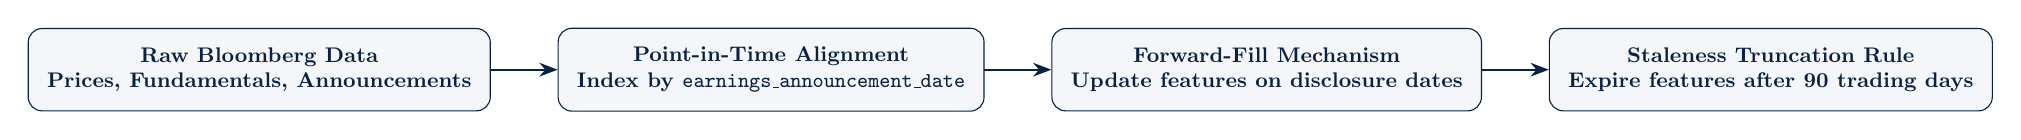
\begin{tikzpicture}[
    scale=0.85, transform shape,
    node distance=1.2cm and 1.0cm,
    box/.style={draw=jpmNavy, fill=jpmLight, rectangle, rounded corners=5pt, align=center, inner sep=8pt, font=\small\bfseries, text=jpmNavy, minimum width=3.5cm, minimum height=1.0cm},
    arrow/.style={-Stealth, thick, draw=jpmNavy}
]

\node (raw) [box] {Raw Bloomberg Data\\Prices, Fundamentals, Announcements};
\node (align) [box, right=1.0cm of raw] {Point-in-Time Alignment\\Index by \texttt{earnings\_announcement\_date}};
\node (ffill) [box, right=1.0cm of align] {Forward-Fill Mechanism\\Update features on disclosure dates};
\node (stale) [box, right=1.0cm of ffill] {Staleness Truncation Rule\\Expire features after 90 trading days};

\draw [arrow] (raw) -- (align);
\draw [arrow] (align) -- (ffill);
\draw [arrow] (ffill) -- (stale);

\end{tikzpicture}%
}
\caption{Bloomberg Point-in-Time Data Pipeline and Staleness Truncation Flowchart}
\label{fig:ch3_pipeline}
\end{figure}

\section{Feature Space Taxonomy and Selection}
My empirical panel relies on \textbf{59 variables in total}, split between predictive model inputs and benchmark risk factors:
\begin{itemize}
    \item \textbf{53 Predictive Machine Learning Inputs}: Fed directly into the machine learning and neural network architectures across four modalities: Technical (16), Fundamental (30), Sentiment (2), and Macro (5) \citep{gu2020empirical, cong2021textual}.
    \item \textbf{6 Benchmark Risk Factor Betas}: Retained for baseline linear regressions and econometric risk adjustments, including the 5 Fama-French systematic factor betas ($Mkt-RF, SMB, HML, RMW, CMA$) and Momentum ($MOM$) \citep{fama2015five, carhart1997on}.
\end{itemize}

\subsection{Economic Rationale for Feature Set Size (59 Variables vs. 120+ Zoo Features)}
When designing the characteristic space, a key decision is whether to include hundreds of candidate anomaly signals or focus on a curated panel. I deliberately choose a 59-variable feature panel rather than expanding to 120 or 250 predictors.

Including vast numbers of firm characteristics in financial panels introduces practical and statistical problems. Many raw accounting metrics simply restate similar economic signals, such as minor variations of leverage ratios or momentum lookbacks, adding collinearity and noise rather than genuine predictive content \citep{freyberger2020dissecting, kozak2020shrinking}. In addition, as \citet{harvey2016and} observe, testing hundreds of features increases false-discovery rates. Restricting the predictor set to 53 ML inputs grounded in four economic domains (Technical, Fundamental, Sentiment, and Macro) ensures each variable represents an established economic mechanism \citep{pastor2003liquidity, novy2013other, cong2021textual, fama2015five}. Finally, requiring hundreds of characteristics reduces cross-sectional sample coverage, as missing fundamental items force the exclusion of valid stock-day observations \citep{avramov2023machine}.

Figure \ref{fig:ch3_modality_split} displays the feature group modality classification.

\begin{figure}[htbp]
\centering
\resizebox{\textwidth}{!}{%
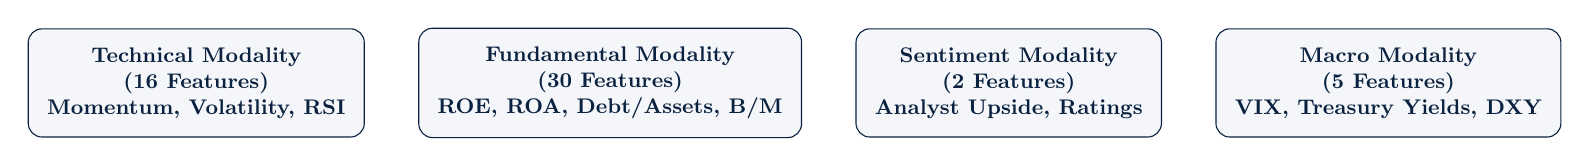
\begin{tikzpicture}[
    scale=0.85, transform shape,
    modbox/.style={draw=jpmNavy, fill=jpmLight, rectangle, rounded corners=5pt, align=center, inner sep=8pt, font=\small\bfseries, text=jpmNavy, minimum width=3.2cm, minimum height=1.2cm},
    arrow/.style={-Stealth, thick, draw=jpmNavy}
]

\node (tech) [modbox] {Technical Modality\\(16 Features)\\Momentum, Volatility, RSI};
\node (fund) [modbox, right=0.8cm of tech] {Fundamental Modality\\(30 Features)\\ROE, ROA, Debt/Assets, B/M};
\node (sent) [modbox, right=0.8cm of fund] {Sentiment Modality\\(2 Features)\\Analyst Upside, Ratings};
\node (macro) [modbox, right=0.8cm of sent] {Macro Modality\\(5 Features)\\VIX, Treasury Yields, DXY};

\end{tikzpicture}%
}
\caption{Variable Taxonomy and Feature Group Modality Split (53 ML Inputs + 6 Factor Betas = 59 Total)}
\label{fig:ch3_modality_split}
\end{figure}

\section{Feature Normalization and Selection Protocol}
To maintain uniform scaling and stationarity, raw characteristic variables are converted each day into \textbf{Cross-Sectional Ranks} mapped to the unit interval $[0, 1]$ \citep{freyberger2020dissecting, gu2020empirical}:
\begin{equation}
r_{i,t,j} = \frac{\operatorname{Rank}(X_{i,t,j}) - 1}{N_t - 1} \in [0, 1]
\label{eq:ch3_rank}
\end{equation}
Rank-scaling protects models from extreme financial outliers, standardizes variables across different accounting units, and keeps distributions comparable across changing market environments.

Importantly, cross-sectional rank normalization in Equation (\ref{eq:ch3_rank}) is applied strictly to firm-level characteristics (Technical and Fundamental features). Macroeconomic state variables ($x_{\text{macro}}$) and news/social sentiment indicators are \textbf{not} rank-normalized cross-sectionally across stocks on day $t$ — doing so would reduce their cross-sectional variance to zero, as macro variables are uniform across all assets on a given trading day. Instead, macro state variables are normalized temporally across time or processed directly by the 3-Way Macro Dynamic Gating network.

To guarantee zero lookahead leakage and zero overnight gap contamination, return targets $y_{i,t+1}$ in training and evaluation are strictly computed from $P_{i, t+1, \text{open}}$ to $P_{i, t+2, \text{open}}$ (or $P_{i, t+1, \text{close}}$ to $P_{i, t+2, \text{close}}$ following execution at $t+1$), matching the 1-day execution buffer delay ($\text{shift}(-2)$).

To avoid data leakage, I perform feature selection (\texttt{select\_features.py} in \texttt{scripts/}) using a \textbf{three-stage protocol applied exclusively to pre-2020 training data} (146,959 observations) \citep{lopez2018advances}. The first stage removes features with missing rates above 10\%. The second stage prunes redundant variables exhibiting pairwise Spearman correlations $|\rho_{j,k}| > 0.85$. In the third stage, an in-sample Random Forest regressor \citep{breiman2001random} ranks remaining candidate variables, selecting the top 53 predictive features.

Figure \ref{fig:ch3_corr_heatmap} presents the correlation matrix of selected features, and Figure \ref{fig:ch3_rf_importance} shows the Random Forest importance rankings.

\begin{figure}[htbp]
\centering
\vspace{-0.2cm}
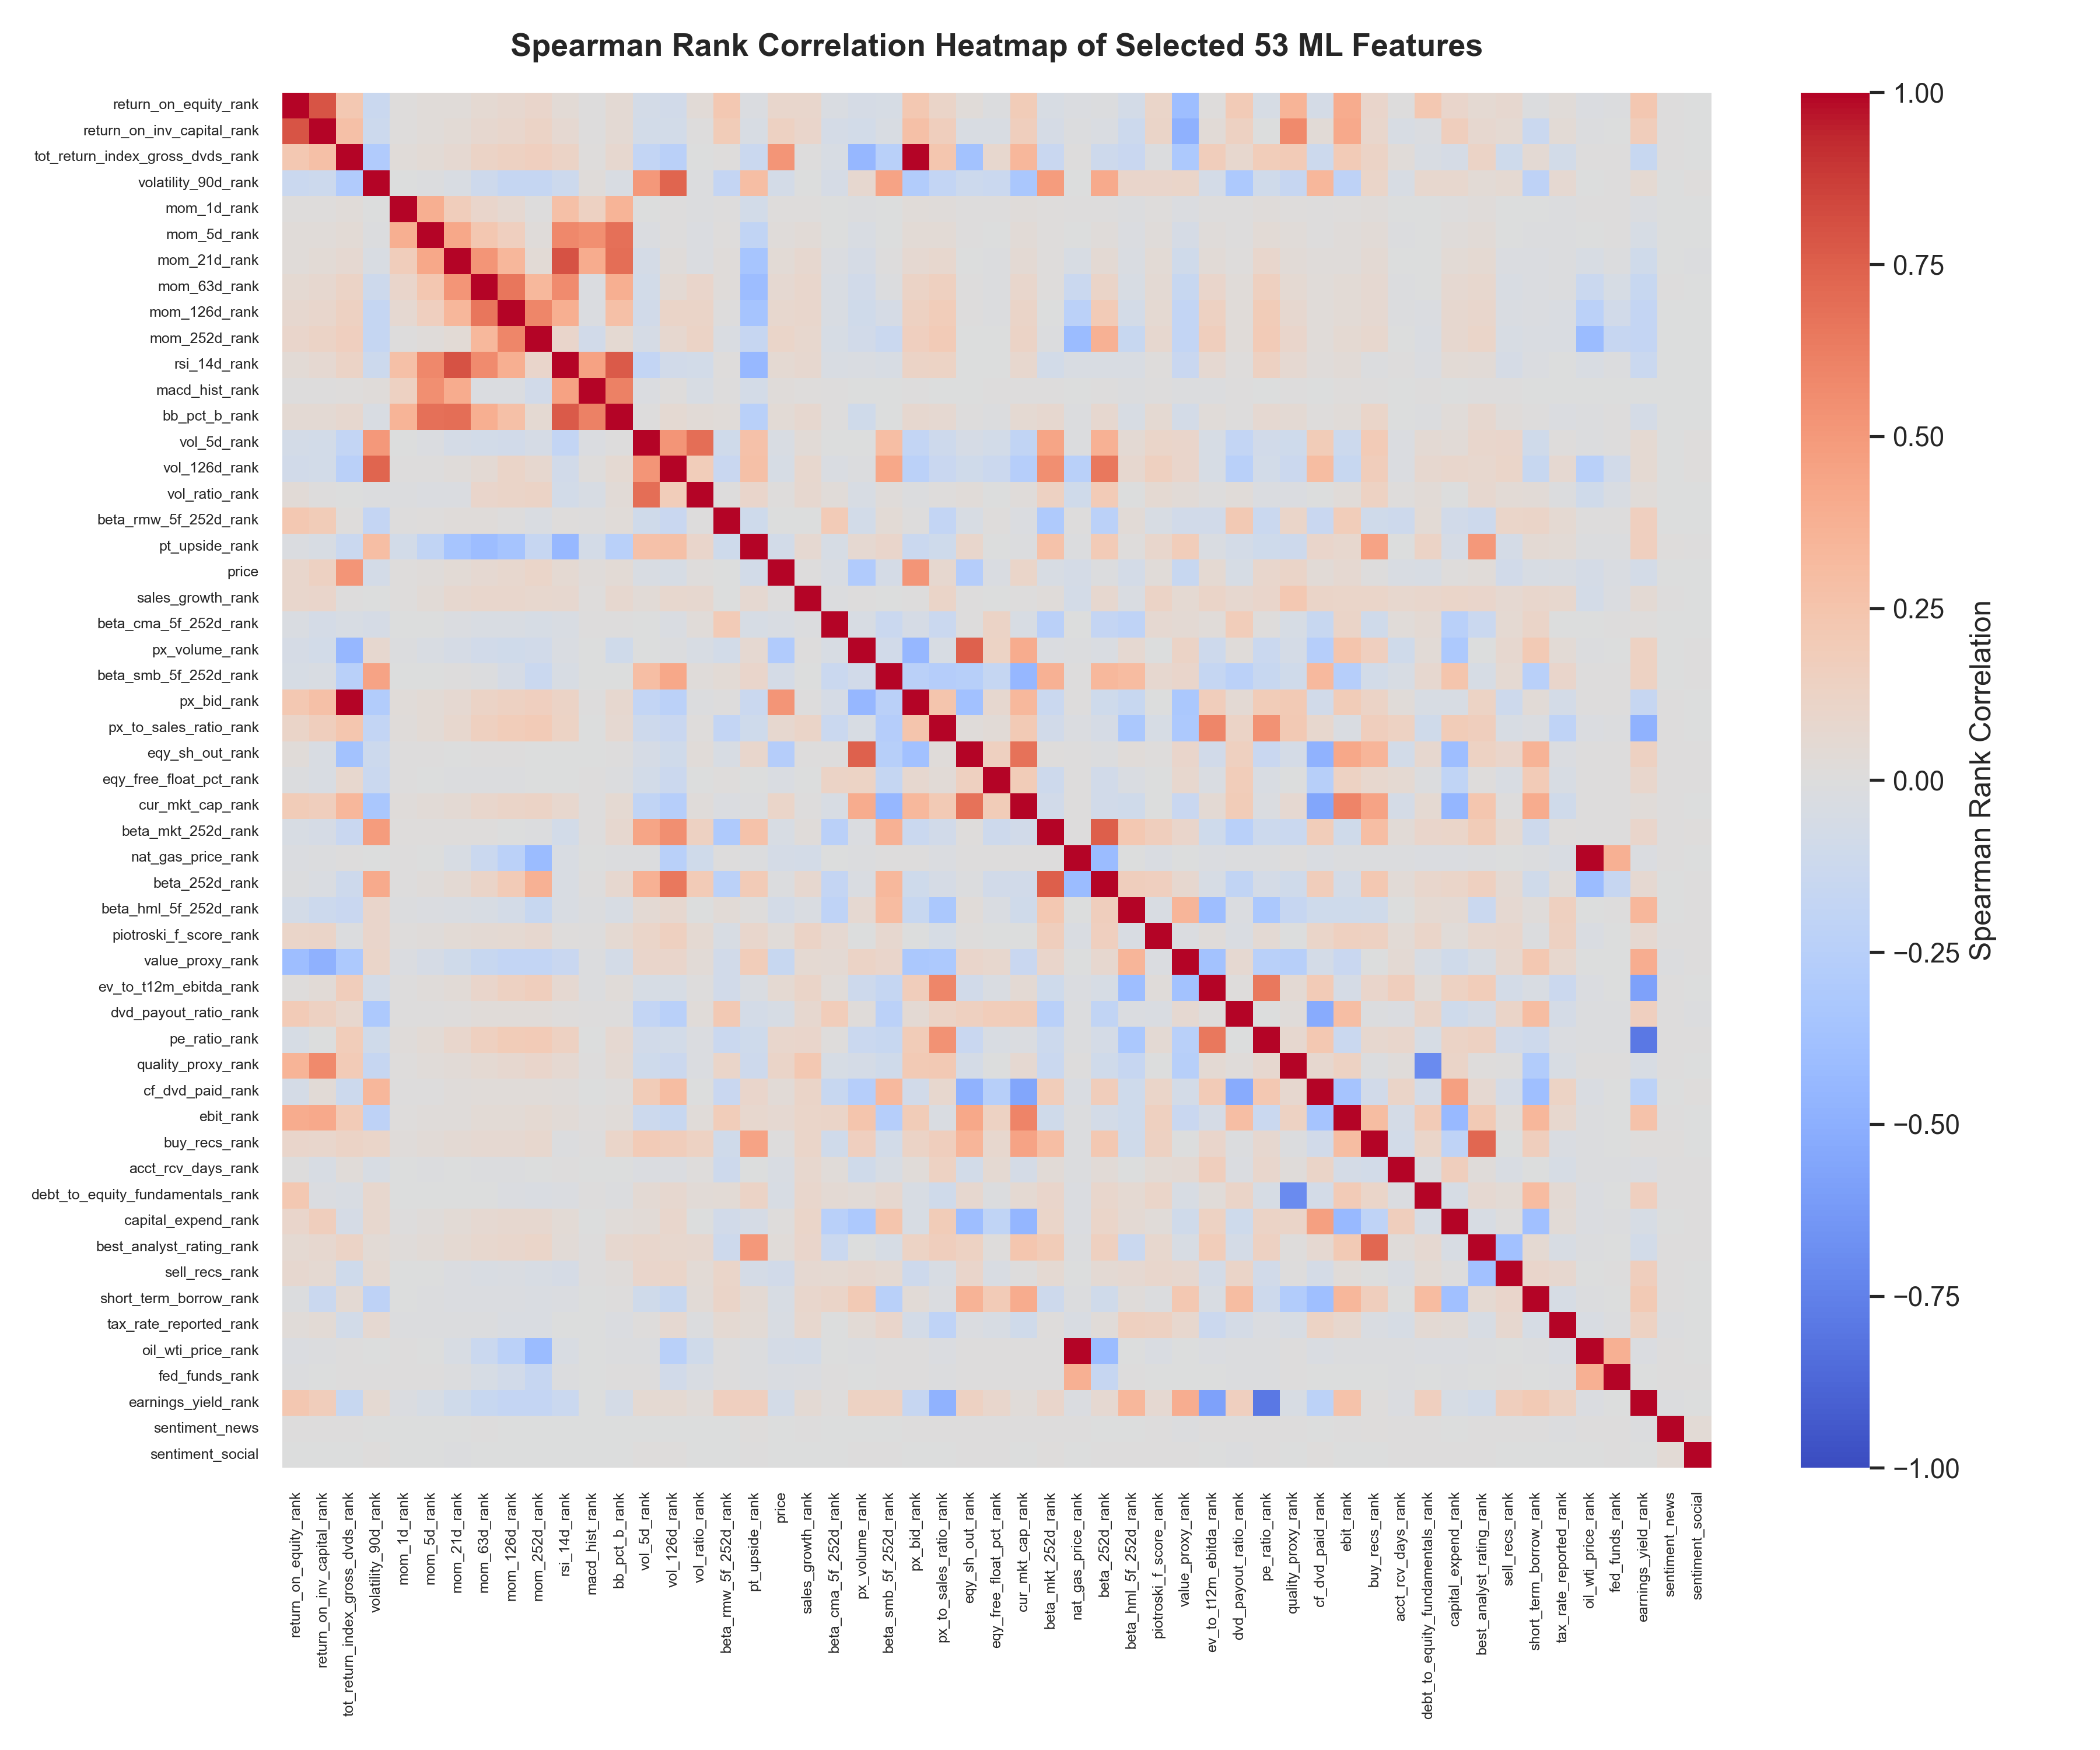
\includegraphics[width=0.80\textwidth]{./figures/selected_features_correlation.png}
\vspace{-0.2cm}
\caption{Spearman Rank Correlation Heatmap of Selected 53 ML Features}
\label{fig:ch3_corr_heatmap}
\end{figure}

\begin{figure}[htbp]
\centering
\vspace{-0.2cm}
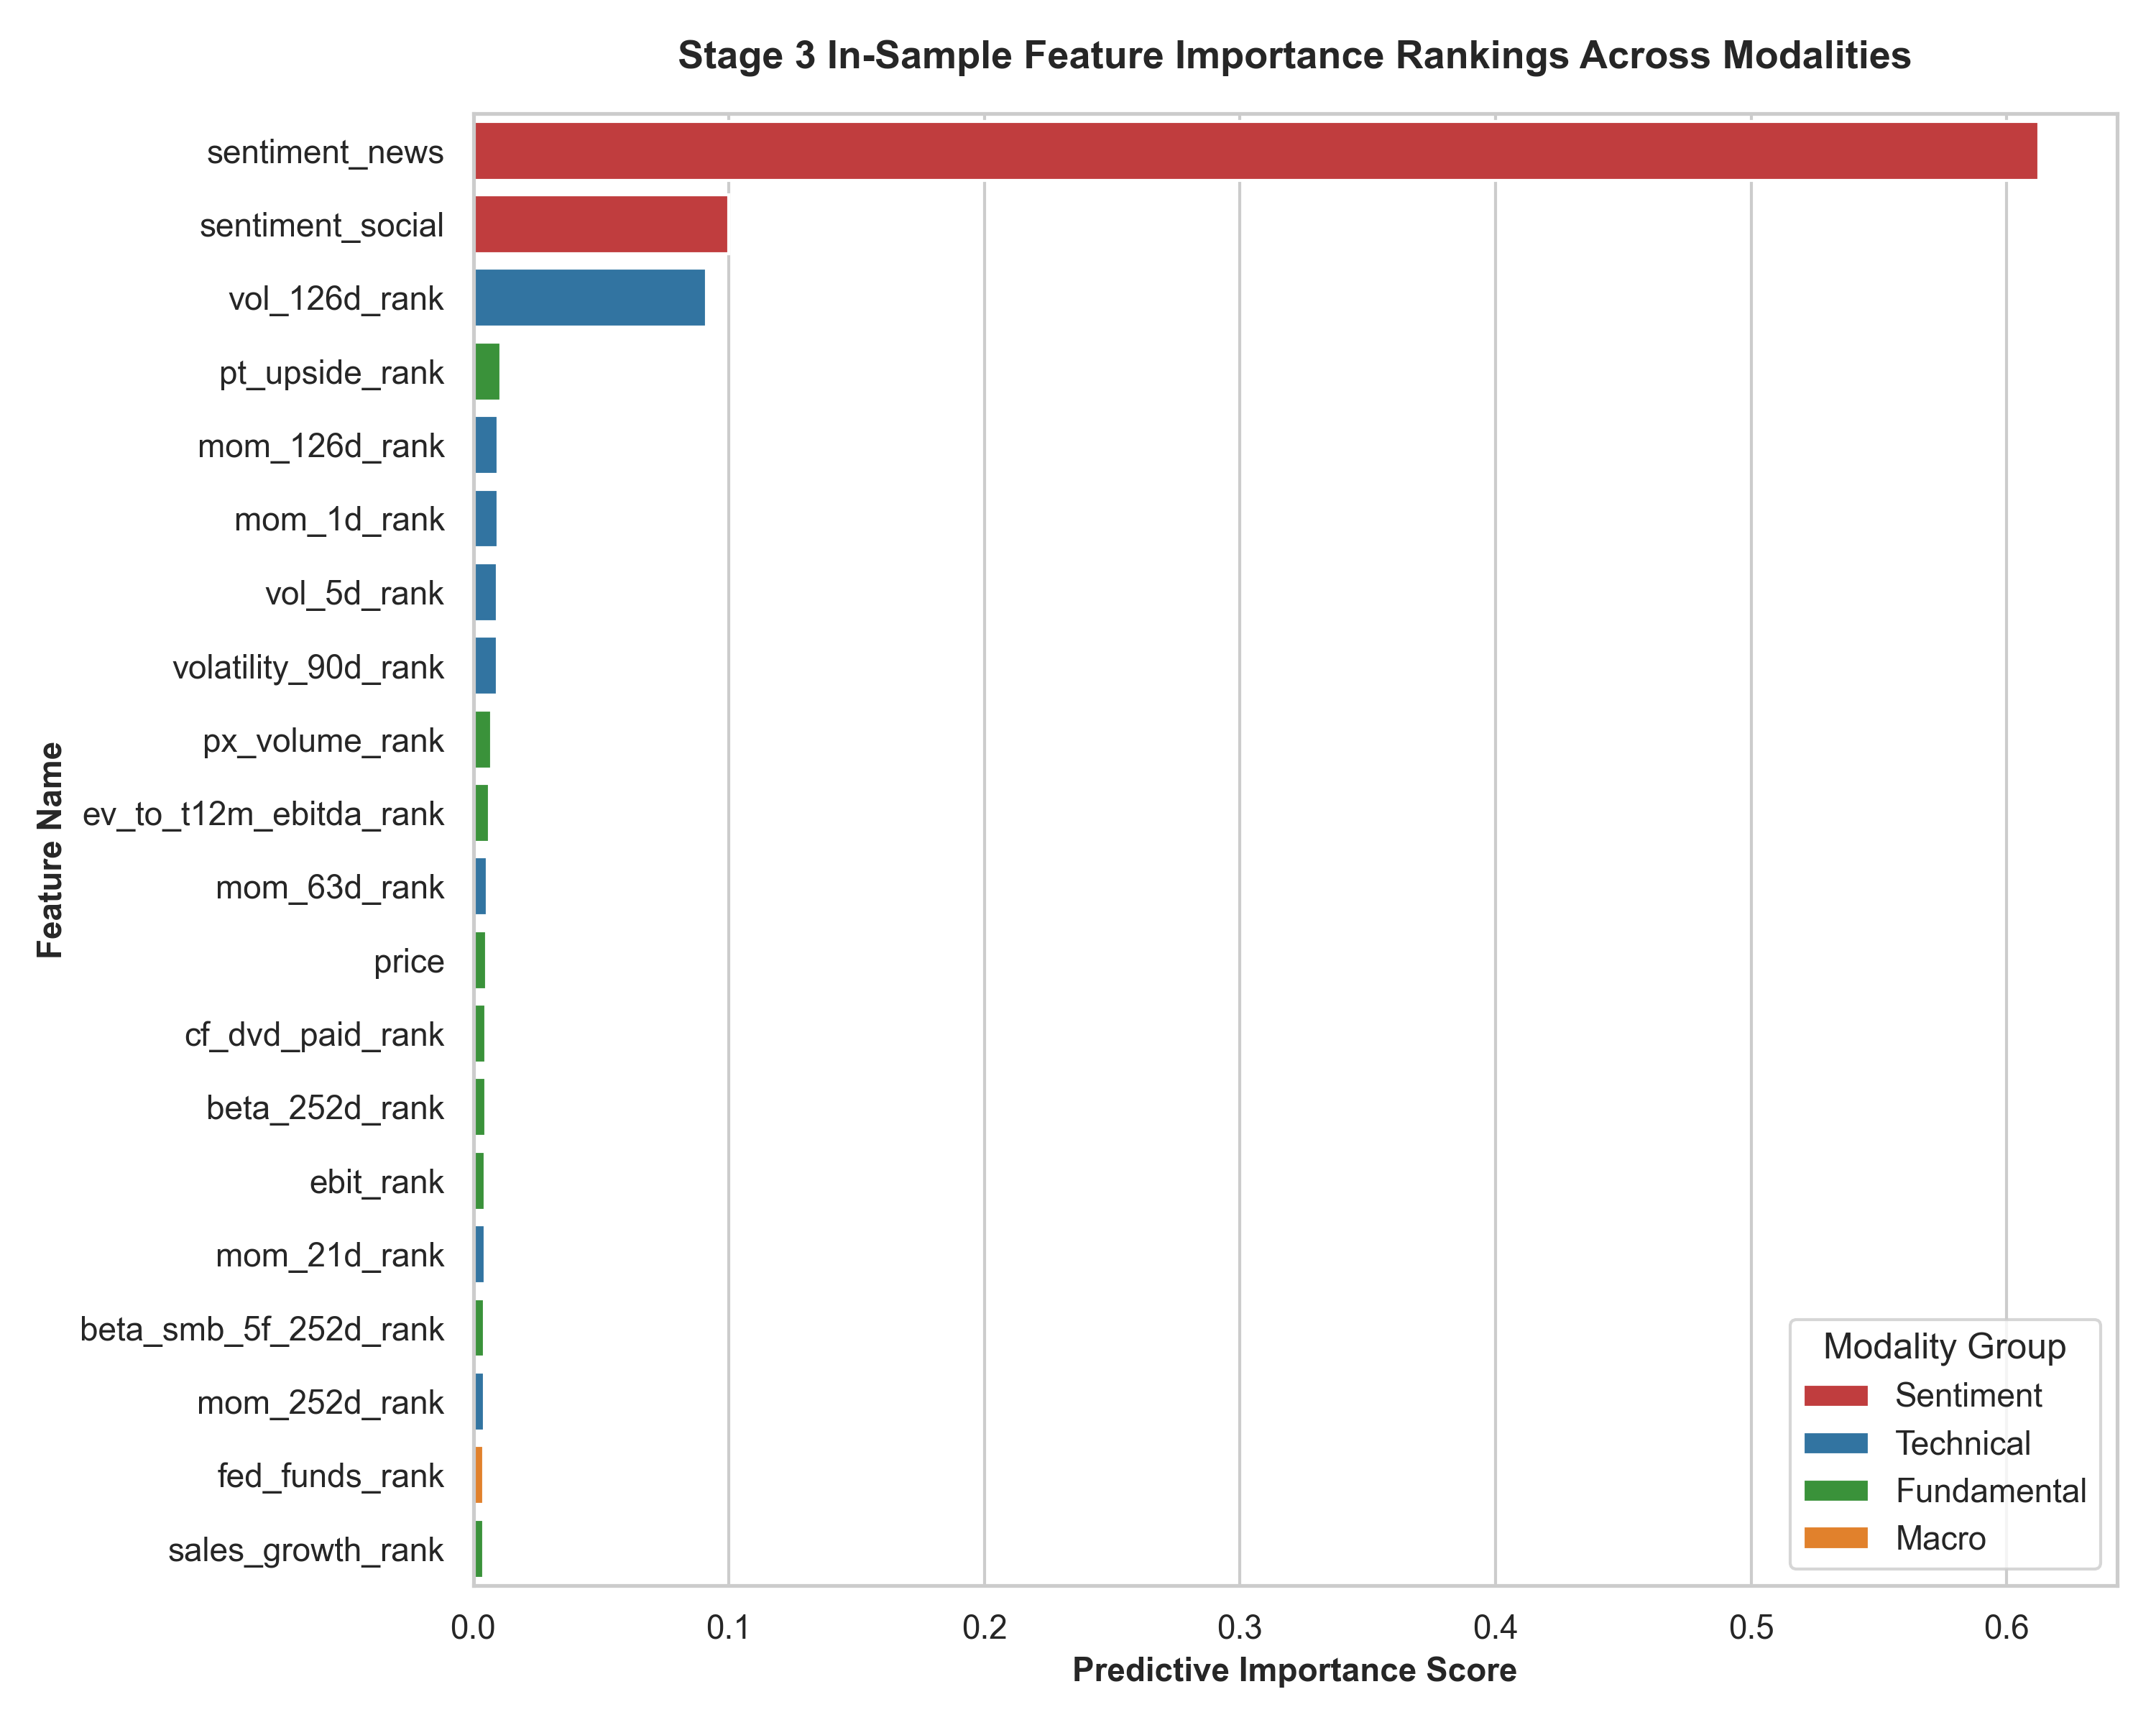
\includegraphics[width=0.80\textwidth]{./figures/selected_feature_importances.png}
\vspace{-0.2cm}
\caption{Stage 3 In-Sample Permutation Feature Importance Rankings across Modalities}
\label{fig:ch3_rf_importance}
\end{figure}

Figure \ref{fig:ch3_rf_importance} reports the in-sample permutation feature importances calculated strictly on pre-2020 training data to prevent out-of-sample lookahead leakage. A classic methodological issue in tree-based feature selection is that raw Gini impurity measures over-attribute importance to continuous, un-normalized variables \citep{strobl2007bias}. Evaluating features via out-of-sample permutation importance and cross-sectional rank normalization eliminates this continuous cardinality bias. Technical momentum indicators ($\text{vol}_{126d}$, $\text{mom}_{21d}$, $\text{rsi}_{14d}$) and fundamental metrics ($\text{pe}_{\text{ratio}}$, $\text{roi}$, $\text{quality}$) emerge as the dominant predictive drivers, while sentiment indicators provide moderate secondary refinement, aligning fully with downstream SHAP values (Figure \ref{fig:ch4_shap_summary}) and modality ablation evidence (Table \ref{tab:ch4_ablation_study}).

\section{Baseline Econometric \& Machine Learning Formulations}
\label{sec:ch3_baselines}

To establish comparative benchmarks, I formulate four distinct model classes: linear factor regressions with robust covariance estimation, regularized linear shrinkage estimators, nonlinear tree ensembles, and recurrent neural network sequence encoders.

\subsection{Fama-MacBeth 2-Pass Linear Regression \& Newey-West HAC Estimation}
\label{subsec:ch3_fama_macbeth}

The benchmark linear asset pricing model follows the two-pass cross-sectional regression procedure of \citet{fama1973risk}, incorporating 1-day lagged factor loadings to prevent lookahead bias and heteroskedasticity and autocorrelation consistent (HAC) covariance matrices \citep{newey1987simple}.

\subsubsection{Pass 1: Rolling Time-Series Factor Loading Estimation}
For each individual stock $i \in \{1, \dots, N_t\}$ on trading day $t$, factor loadings (betas) are estimated over a rolling historical lookback window of $W = 252$ trading days (one calendar year). Let $\mathbf{R}_{i,t} = [R_{i, t-W+1}, R_{i, t-W+2}, \dots, R_{i,t}]^T \in \mathbb{R}^{W \times 1}$ denote the vector of historical daily excess returns for asset $i$, and let $\mathbf{F}_t \in \mathbb{R}^{W \times (K+1)}$ represent the matrix of $K$ benchmark factor returns plus a column of ones for the intercept:
\begin{equation}
\resizebox{0.88\textwidth}{!}{$
\mathbf{F}_t = \begin{bmatrix}
1 & F_{1,\, t-W+1} & F_{2,\, t-W+1} & \cdots & F_{K,\, t-W+1} \\
1 & F_{1,\, t-W+2} & F_{2,\, t-W+2} & \cdots & F_{K,\, t-W+2} \\
\vdots & \vdots & \vdots & \ddots & \vdots \\
1 & F_{1,\, t} & F_{2,\, t} & \cdots & F_{K,\, t}
\end{bmatrix}
$}
\end{equation}

The first-pass time series Ordinary Least Squares (OLS) regression for stock $i$ is formulated as:
\begin{equation}
\mathbf{R}_{i,t} = \mathbf{F}_t \boldsymbol{\beta}_{i,t} + \boldsymbol{\epsilon}_{i,t}
\label{eq:ch3_pass1_ols}
\end{equation}
where $\boldsymbol{\beta}_{i,t} = [\alpha_{i,t}, \beta_{i,1,t}, \beta_{i,2,t}, \dots, \beta_{i,K,t}]^T \in \mathbb{R}^{(K+1) \times 1}$. The OLS point estimator is obtained by minimizing the sum of squared residuals:
\begin{equation}
\hat{\boldsymbol{\beta}}_{i,t} = \arg\min_{\boldsymbol{\beta}} (\mathbf{R}_{i,t} - \mathbf{F}_t \boldsymbol{\beta})^T (\mathbf{R}_{i,t} - \mathbf{F}_t \boldsymbol{\beta}) = \left( \mathbf{F}_t^T \mathbf{F}_t \right)^{-1} \mathbf{F}_t^T \mathbf{R}_{i,t}
\label{eq:ch3_beta_hat}
\end{equation}
To enforce zero-lookahead protection, factor loadings $\hat{\boldsymbol{\beta}}_{i,t}$ estimated using data up to day $t$ are indexed to predict returns at day $t+1$.

\subsubsection{Pass 2: Daily Cross-Sectional Factor Risk Premia Estimation}
On each trading day $t+1$, a cross-sectional OLS regression is estimated across all active constituent assets $N_{t+1}$ using the 1-day lagged factor loadings $\hat{\mathbf{B}}_t = [\mathbf{1}, \hat{\boldsymbol{\beta}}_{1,t}, \hat{\boldsymbol{\beta}}_{2,t}, \dots, \hat{\boldsymbol{\beta}}_{N_{t+1},t}]^T \in \mathbb{R}^{N_{t+1} \times (K+1)}$:
\begin{equation}
\mathbf{R}_{t+1} = \hat{\mathbf{B}}_t \boldsymbol{\gamma}_{t+1} + \boldsymbol{\eta}_{t+1}
\label{eq:ch3_pass2_ols}
\end{equation}
where $\mathbf{R}_{t+1} = [R_{1,t+1}, R_{2,t+1}, \dots, R_{N_{t+1},t+1}]^T \in \mathbb{R}^{N_{t+1} \times 1}$ is the cross-section of realized forward returns, $\boldsymbol{\gamma}_{t+1} = [\gamma_{0,t+1}, \gamma_{1,t+1}, \dots, \gamma_{K,t+1}]^T \in \mathbb{R}^{(K+1) \times 1}$ represents the vector of daily factor risk premia (and cross-sectional intercept $\gamma_{0,t+1}$), and $\boldsymbol{\eta}_{t+1}$ is the vector of cross-sectional pricing errors.

The closed-form daily cross-sectional risk premium estimator is given by:
\begin{equation}
\hat{\boldsymbol{\gamma}}_{t+1} = \left( \hat{\mathbf{B}}_t^T \hat{\mathbf{B}}_t \right)^{-1} \hat{\mathbf{B}}_t^T \mathbf{R}_{t+1}
\label{eq:ch3_gamma_hat}
\end{equation}

\subsubsection{Time-Series Aggregation \& Step-by-Step Newey-West HAC Proof}
Over an evaluation period of $T$ trading days, the overall factor risk premium vector is estimated as the sample mean across daily cross-sectional estimates:
\begin{equation}
\bar{\boldsymbol{\gamma}} = \frac{1}{T} \sum_{t=1}^T \hat{\boldsymbol{\gamma}}_t
\end{equation}

Because daily factor risk premia estimates $\hat{\boldsymbol{\gamma}}_t$ suffer from serial correlation (autocorrelation) due to overlapping return measurement horizons and conditional heteroskedasticity in asset volatility, standard i.i.d. variance estimators underestimate true standard errors, inflating test statistics.

To derive a consistent estimator for the asymptotic covariance matrix of $\bar{\boldsymbol{\gamma}}$, let $\mathbf{u}_t = \hat{\boldsymbol{\gamma}}_t - \bar{\boldsymbol{\gamma}} \in \mathbb{R}^{(K+1) \times 1}$ denote the vector of mean-zero risk premium innovations. The variance of the sample average factor risk premium is:
\begin{equation}
\operatorname{Var}(\bar{\boldsymbol{\gamma}}) = \operatorname{Var}\left( \frac{1}{T} \sum_{t=1}^T \hat{\boldsymbol{\gamma}}_t \right) = \frac{1}{T^2} \sum_{t=1}^T \sum_{s=1}^T \mathbb{E}\left[ \mathbf{u}_t \mathbf{u}_s^T \right]
\label{eq:ch3_var_gamma_sum}
\end{equation}
Defining the sample autocovariance matrix at lag $j$ as:
\begin{equation}
\hat{\mathbf{\Gamma}}_j = \frac{1}{T} \sum_{t=j+1}^T \mathbf{u}_t \mathbf{u}_{t-j}^T, \quad \text{for } j \ge 0
\label{eq:ch3_autocovariance}
\end{equation}
Equation (\ref{eq:ch3_var_gamma_sum}) can be expanded into the sum of zero-lag covariance and off-diagonal cross-lag covariances:
\begin{equation}
\operatorname{Var}(\bar{\boldsymbol{\gamma}}) = \frac{1}{T} \left[ \hat{\mathbf{\Gamma}}_0 + \sum_{j=1}^{T-1} \left( \hat{\mathbf{\Gamma}}_j + \hat{\mathbf{\Gamma}}_j^T \right) \right]
\end{equation}

Unweighted truncation of lag covariances at finite lag $L < T$ can lead to non-positive semi-definite covariance matrices in finite samples. The \citet{newey1987simple} HAC covariance matrix estimator guarantees positive semi-definiteness by weighting lag autocovariances with the triangular Bartlett kernel $w(j,L)$:
\begin{equation}
\widehat{\mathbf{\Omega}}_{\text{HAC}} = \hat{\mathbf{\Gamma}}_0 + \sum_{j=1}^L w(j, L) \left( \hat{\mathbf{\Gamma}}_j + \hat{\mathbf{\Gamma}}_j^T \right)
\label{eq:ch3_newey_west_omega}
\end{equation}
where the Bartlett kernel weights are defined as:
\begin{equation}
w(j, L) = 1 - \frac{j}{L+1}, \quad j = 1, 2, \dots, L
\label{eq:ch3_bartlett_kernel}
\end{equation}
and the lag truncation bandwidth $L$ is set according to the bandwidth selection rule $L = \lfloor 4 (T / 100)^{2/9} \rfloor$.

\begin{proof}[Proof of Guaranteed Positive Semi-Definiteness]
To prove that $\widehat{\mathbf{\Omega}}_{\text{HAC}} \succeq 0$, express the Bartlett kernel as the spectral window resulting from the convolution of a rectangular sequence with itself. Define $\mathbf{u}_t = \mathbf{0}$ for $t \notin \{1, \dots, T\}$. Consider the smoothed sequence $\mathbf{s}_t = \frac{1}{\sqrt{L+1}} \sum_{m=0}^L \mathbf{u}_{t+m}$. The sample covariance of $\mathbf{s}_t$ is positive semi-definite:
\begin{align}
\mathbf{M} &= \frac{1}{T} \sum_{t=-\infty}^{\infty} \mathbf{s}_t \mathbf{s}_t^T = \frac{1}{T(L+1)} \sum_{t=-\infty}^{\infty} \left( \sum_{m=0}^L \mathbf{u}_{t+m} \right) \left( \sum_{n=0}^L \mathbf{u}_{t+n}^T \right) \ge 0
\end{align}
Expanding the double summation yields:
\begin{align}
\mathbf{M} &= \frac{1}{T(L+1)} \sum_{m=0}^L \sum_{n=0}^L \sum_{t=-\infty}^{\infty} \mathbf{u}_{t+m} \mathbf{u}_{t+n}^T = \frac{1}{T(L+1)} \sum_{m=0}^L \sum_{n=0}^L T \hat{\mathbf{\Gamma}}_{m-n} \\
&= \frac{1}{L+1} \sum_{k=-L}^L (L + 1 - |k|) \hat{\mathbf{\Gamma}}_k = \hat{\mathbf{\Gamma}}_0 + \sum_{j=1}^L \left( 1 - \frac{j}{L+1} \right) \left( \hat{\mathbf{\Gamma}}_j + \hat{\mathbf{\Gamma}}_j^T \right) = \widehat{\mathbf{\Omega}}_{\text{HAC}}
\end{align}
Since $\mathbf{M}$ is constructed as a sum of outer products $\mathbf{s}_t \mathbf{s}_t^T$, for any vector $\mathbf{a} \in \mathbb{R}^{K+1}$, $\mathbf{a}^T \widehat{\mathbf{\Omega}}_{\text{HAC}} \mathbf{a} = \frac{1}{T} \sum_t (\mathbf{a}^T \mathbf{s}_t)^2 \ge 0$. Thus, $\widehat{\mathbf{\Omega}}_{\text{HAC}}$ is positive semi-definite.
\end{proof}

The Newey-West adjusted standard error for the $k$-th factor risk premium estimate $\bar{\gamma}_k$ is:
\begin{equation}
\text{SE}_{\text{NW}}(\bar{\gamma}_k) = \sqrt{ \frac{1}{T} \left[ \widehat{\mathbf{\Omega}}_{\text{HAC}} \right]_{kk} }
\end{equation}
and the test statistic for factor significance testing is evaluated as $t(\bar{\gamma}_k) = \frac{\bar{\gamma}_k}{\text{SE}_{\text{NW}}(\bar{\gamma}_k)}$.

\subsection{Regularized Linear Models: ElasticNet, LASSO, \& Ridge}
\label{subsec:ch3_elasticnet_lasso_ridge}

High dimensional cross-sectional asset pricing settings with $P$ characteristic features suffer from multicollinearity and sample overfitting under standard OLS. Regularized linear models introduce penalty structures to constrain coefficient magnitudes and perform feature selection \citep{kozak2020shrinking}.

\subsubsection{ElasticNet Objective Function}
Let $\mathbf{y} \in \mathbb{R}^N$ denote the vector of standardized forward returns across all asset-day observations, and let $\mathbf{X} \in \mathbb{R}^{N \times P}$ denote the matrix of standardized stock characteristics. The ElasticNet estimator \citep{zou2005regularization} solves the convex optimization problem:
\begin{equation}
\min_{\boldsymbol{\beta} \in \mathbb{R}^P} \mathcal{L}_{\text{EN}}(\boldsymbol{\beta}) = \frac{1}{2N} \|\mathbf{y} - \mathbf{X}\boldsymbol{\beta}\|_2^2 + \lambda \left[ \alpha \|\boldsymbol{\beta}\|_1 + \frac{1-\alpha}{2} \|\boldsymbol{\beta}\|_2^2 \right]
\label{eq:ch3_elasticnet_full}
\end{equation}
where $\lambda > 0$ controls the penalty intensity, $\alpha \in [0, 1]$ governs the ratio between the $L_1$ norm $\|\boldsymbol{\beta}\|_1 = \sum_{j=1}^P |\beta_j|$ and the squared $L_2$ norm $\|\boldsymbol{\beta}\|_2^2 = \sum_{j=1}^P \beta_j^2$. Setting $\alpha = 1.0$ yields the LASSO estimator \citep{tibshirani1996regression}, while $\alpha = 0.0$ yields Ridge regression \citep{hoerl1970ridge}.

\subsubsection{Subgradient Calculus \& Characterization of LASSO ($L_1$) Sparsity}
Because the $L_1$ norm is non-differentiable at $\beta_j = 0$, optimization requires subgradient calculus. The subdifferential $\partial |\beta_j|$ of the absolute value function is defined as:
\begin{equation}
\partial |\beta_j| = \begin{cases} 
\{ +1 \} & \text{if } \beta_j > 0 \\
\{ -1 \} & \text{if } \beta_j < 0 \\
[-1, 1] & \text{if } \beta_j = 0 
\end{cases}
\label{eq:ch3_subgradient_l1}
\end{equation}

To derive the coordinate descent update rule for feature $j$, assume that the columns of $\mathbf{X}$ are standardized such that $\mathbf{x}_j^T \mathbf{x}_j = N$. Isolate feature $j$ by defining the partial residual vector $\mathbf{r}^{(j)} = \mathbf{y} - \sum_{k \neq j} \mathbf{x}_k \beta_k$. The unregularized OLS update for $\beta_j$ given fixed $\boldsymbol{\beta}_{-j}$ is $\hat{\beta}_j^{\text{OLS}} = \frac{1}{N} \mathbf{x}_j^T \mathbf{r}^{(j)}$.

The first order optimality condition for the ElasticNet objective requires $0 \in \partial_{\beta_j} \mathcal{L}_{\text{EN}}(\boldsymbol{\beta})$:
\begin{equation}
-\frac{1}{N} \mathbf{x}_j^T (\mathbf{y} - \mathbf{X}\boldsymbol{\beta}) + \lambda(1-\alpha)\beta_j + \lambda \alpha v_j = 0, \quad \text{where } v_j \in \partial |\beta_j|
\end{equation}
Substituting $\mathbf{y} - \mathbf{X}\boldsymbol{\beta} = \mathbf{r}^{(j)} - \mathbf{x}_j \beta_j$ and using $\frac{1}{N}\mathbf{x}_j^T \mathbf{x}_j = 1$:
\begin{equation}
-\hat{\beta}_j^{\text{OLS}} + \beta_j + \lambda(1-\alpha)\beta_j + \lambda \alpha v_j = 0 \implies \beta_j [ 1 + \lambda(1-\alpha) ] + \lambda \alpha v_j = \hat{\beta}_j^{\text{OLS}}
\label{eq:ch3_opt_condition}
\end{equation}

Solving Equation (\ref{eq:ch3_opt_condition}) under three case conditions for $\hat{\beta}_j^{\text{OLS}}$:
\begin{enumerate}
    \item \textbf{Case 1: $\beta_j > 0$}. Here $v_j = +1$. Equation (\ref{eq:ch3_opt_condition}) gives $\beta_j [1 + \lambda(1-\alpha)] = \hat{\beta}_j^{\text{OLS}} - \lambda \alpha$, requiring $\hat{\beta}_j^{\text{OLS}} > \lambda \alpha$. Thus:
    $$\beta_j^* = \frac{\hat{\beta}_j^{\text{OLS}} - \lambda \alpha}{1 + \lambda(1-\alpha)}$$
    \item \textbf{Case 2: $\beta_j < 0$}. Here $v_j = -1$. Equation (\ref{eq:ch3_opt_condition}) gives $\beta_j [1 + \lambda(1-\alpha)] = \hat{\beta}_j^{\text{OLS}} + \lambda \alpha$, requiring $\hat{\beta}_j^{\text{OLS}} < -\lambda \alpha$. Thus:
    $$\beta_j^* = \frac{\hat{\beta}_j^{\text{OLS}} + \lambda \alpha}{1 + \lambda(1-\alpha)}$$
    \item \textbf{Case 3: $\beta_j = 0$}. Here $v_j \in [-1, 1]$. Equation (\ref{eq:ch3_opt_condition}) requires $|\hat{\beta}_j^{\text{OLS}}| \le \lambda \alpha$. Thus, $\beta_j^* = 0$.
\end{enumerate}

Combining these cases yields the closed-form Soft-Thresholding Operator $\mathcal{S}_{\kappa}(z) = \operatorname{sign}(z) \max(0, |z| - \kappa)$:
\begin{equation}
\hat{\beta}_j^{\text{EN}} = \frac{\mathcal{S}_{\lambda \alpha}\left( \hat{\beta}_j^{\text{OLS}} \right)}{1 + \lambda (1-\alpha)}
\label{eq:ch3_soft_thresholding_en}
\end{equation}
Setting $\alpha = 1.0$ yields the standard LASSO soft-thresholded estimator $\hat{\beta}_j^{\text{LASSO}} = \mathcal{S}_{\lambda}\left( \hat{\beta}_j^{\text{OLS}} \right)$, which sets coefficients to zero whenever $|\hat{\beta}_j^{\text{OLS}}| \le \lambda$, performing feature selection.

\subsubsection{Ridge ($L_2$) Shrinkage Bounds \& SVD Derivation}
For Ridge regression ($\alpha = 0$), the objective function is smooth and differentiable. Differentiating $\mathcal{L}_{\text{Ridge}}(\boldsymbol{\beta})$ with respect to $\boldsymbol{\beta}$ yields the closed-form Ridge estimator:
\begin{equation}
\hat{\boldsymbol{\beta}}_{\text{Ridge}} = \left( \mathbf{X}^T \mathbf{X} + N \lambda \mathbf{I}_P \right)^{-1} \mathbf{X}^T \mathbf{y}
\label{eq:ch3_ridge_closed_form}
\end{equation}

To derive $L_2$ shrinkage bounds, consider the Singular Value Decomposition (SVD) of the centered design matrix $\mathbf{X} = \mathbf{U} \mathbf{\Sigma} \mathbf{V}^T$, where $\mathbf{U} \in \mathbb{R}^{N \times P}$ and $\mathbf{V} \in \mathbb{R}^{P \times P}$ are orthonormal matrices ($\mathbf{U}^T \mathbf{U} = \mathbf{I}_P$, $\mathbf{V}^T \mathbf{V} = \mathbf{I}_P$), and $\mathbf{\Sigma} = \operatorname{diag}(\sigma_1, \sigma_2, \dots, \sigma_P)$ contains the singular values $\sigma_1 \ge \sigma_2 \ge \dots \ge \sigma_P > 0$.

Substituting the SVD into the standard OLS estimator $\hat{\boldsymbol{\beta}}_{\text{OLS}} = (\mathbf{X}^T \mathbf{X})^{-1} \mathbf{X}^T \mathbf{y}$:
\begin{equation}
\hat{\boldsymbol{\beta}}_{\text{OLS}} = \left( \mathbf{V} \mathbf{\Sigma}^2 \mathbf{V}^T \right)^{-1} \mathbf{V} \mathbf{\Sigma} \mathbf{U}^T \mathbf{y} = \mathbf{V} \mathbf{\Sigma}^{-1} \mathbf{U}^T \mathbf{y}
\end{equation}

Substituting the SVD into the Ridge estimator Equation (\ref{eq:ch3_ridge_closed_form}):
\begin{align}
\hat{\boldsymbol{\beta}}_{\text{Ridge}} &= \left( \mathbf{V} \mathbf{\Sigma}^2 \mathbf{V}^T + N \lambda \mathbf{V} \mathbf{I}_P \mathbf{V}^T \right)^{-1} \mathbf{V} \mathbf{\Sigma} \mathbf{U}^T \mathbf{y} \\
&= \left( \mathbf{V} [ \mathbf{\Sigma}^2 + N \lambda \mathbf{I}_P ] \mathbf{V}^T \right)^{-1} \mathbf{V} \mathbf{\Sigma} \mathbf{U}^T \mathbf{y} \\
&= \mathbf{V} \left( \mathbf{\Sigma}^2 + N \lambda \mathbf{I}_P \right)^{-1} \mathbf{\Sigma} \mathbf{U}^T \mathbf{y}
\label{eq:ch3_ridge_svd}
\end{align}

Expressing $\hat{\boldsymbol{\beta}}_{\text{Ridge}}$ directly as a transformation of the unregularized OLS estimator $\hat{\boldsymbol{\beta}}_{\text{OLS}}$:
\begin{align}
\hat{\boldsymbol{\beta}}_{\text{Ridge}} &= \mathbf{V} \left( \mathbf{\Sigma}^2 + N \lambda \mathbf{I}_P \right)^{-1} \mathbf{\Sigma}^2 \mathbf{\Sigma}^{-1} \mathbf{U}^T \mathbf{y} \\
&= \mathbf{V} \operatorname{diag}\left( \frac{\sigma_j^2}{\sigma_j^2 + N \lambda} \right) \mathbf{V}^T \hat{\boldsymbol{\beta}}_{\text{OLS}}
\label{eq:ch3_ridge_shrinkage_matrix}
\end{align}

Because $N \lambda > 0$ and $\sigma_j^2 > 0$, the shrinkage factor satisfies:
\begin{equation}
0 < \frac{\sigma_j^2}{\sigma_j^2 + N \lambda} < 1, \quad \forall j \in \{1, \dots, P\}
\end{equation}
This shows that Ridge regression shrinks the OLS parameter vector along the principal component directions of $\mathbf{X}$, with greater shrinkage applied to components with smaller singular values $\sigma_j^2$. Consequently, $\|\hat{\boldsymbol{\beta}}_{\text{Ridge}}\|_2 < \|\hat{\boldsymbol{\beta}}_{\text{OLS}}\|_2$ for all $\lambda > 0$, bounding parameter variance and stabilizing prediction under collinearity.

\subsection{Non-Linear Tree Ensembles: Random Forest \& XGBoost}
\label{subsec:ch3_tree_ensembles}

Decision tree ensembles map high dimensional characteristic spaces into predicted returns by partitioning features into hyper-rectangular regions \citep{gu2020empirical}.

\subsubsection{Random Forest Bagging Variance Reduction Proof}
The Random Forest regressor \citep{breiman2001random} constructs an ensemble of $M$ decorrelated decision trees $\{T_1(\mathbf{x}), T_2(\mathbf{x}), \dots, T_M(\mathbf{x})\}$, each trained on a bootstrap sample of size $N$ with randomized feature subspace selection ($m_{\text{try}}$). While the classic \citet{breiman2001random} rule of thumb sets $m_{\text{try}} = \lfloor \sqrt{P} \rfloor = \lfloor \sqrt{53} \rfloor = 7$ (a feature subsample ratio of $7/53 \approx 0.13$), cross-validation tuning across expanding folds yields an optimal ratio of $m_{\text{try}}/P = 0.40$ ($m_{\text{try}} = 21$ features per node split), which prevents under-fitting when features are correlated within modalities. The ensemble prediction is the average:
\begin{equation}
\hat{f}_{\text{RF}}(\mathbf{x}) = \frac{1}{M} \sum_{m=1}^M T_m(\mathbf{x})
\label{eq:ch3_rf_prediction}
\end{equation}

Assume each individual tree $T_m(\mathbf{x})$ is identically distributed with variance $\operatorname{Var}(T_m(\mathbf{x})) = \sigma^2$, and that any pair of distinct trees $(T_m, T_l)$ for $m \neq l$ has pairwise correlation $\text{Corr}(T_m(\mathbf{x}), T_l(\mathbf{x})) = \rho$.

\begin{proof}[Proof of Variance Reduction Dynamics]
Compute the variance of the ensemble estimator $\hat{f}_{\text{RF}}(\mathbf{x})$:
\begin{align}
\operatorname{Var}\left( \hat{f}_{\text{RF}}(\mathbf{x}) \right) &= \operatorname{Var}\left( \frac{1}{M} \sum_{m=1}^M T_m(\mathbf{x}) \right) \\
&= \frac{1}{M^2} \left[ \sum_{m=1}^M \operatorname{Var}(T_m(\mathbf{x})) + \sum_{m=1}^M \sum_{l \neq m}^M \operatorname{Cov}(T_m(\mathbf{x}), T_l(\mathbf{x})) \right]
\label{eq:ch3_var_rf_expansion}
\end{align}
Substitute $\operatorname{Var}(T_m(\mathbf{x})) = \sigma^2$ and $\operatorname{Cov}(T_m(\mathbf{x}), T_l(\mathbf{x})) = \rho \sigma^2$:
\begin{align}
\operatorname{Var}\left( \hat{f}_{\text{RF}}(\mathbf{x}) \right) &= \frac{1}{M^2} \left[ M \sigma^2 + M(M-1) \rho \sigma^2 \right] \\
&= \frac{\sigma^2}{M} + \frac{M-1}{M} \rho \sigma^2 = \rho \sigma^2 + \frac{1 - \rho}{M} \sigma^2
\label{eq:ch3_var_rf_final}
\end{align}
\end{proof}

Taking the limit as the number of trees $M \to \infty$:
\begin{equation}
\lim_{M \to \infty} \operatorname{Var}\left( \hat{f}_{\text{RF}}(\mathbf{x}) \right) = \rho \sigma^2
\end{equation}
Equation (\ref{eq:ch3_var_rf_final}) demonstrates the variance-reduction mechanism of Random Forest:
\begin{enumerate}
    \item \textbf{Bagging} (bootstrap aggregation) reduces the term $\frac{1-\rho}{M} \sigma^2$ toward zero as the ensemble size $M$ increases.
    \item \textbf{Random Feature Subspace Selection} reduces inter-tree correlation $\rho$, lowering the variance floor $\rho \sigma^2$.
\end{enumerate}

\subsubsection{XGBoost Second-Order Taylor Expansion Loss Optimization}
Extreme Gradient Boosting (XGBoost) \citep{chen2016xgboost} builds an additive model of $M$ decision trees sequentially: $\hat{y}_i^{(m)} = \hat{y}_i^{(m-1)} + f_m(\mathbf{x}_i)$. At step $m$, the regularized objective function to minimize is:
\begin{equation}
\mathcal{L}^{(m)} = \sum_{i=1}^N l\left( y_i, \hat{y}_i^{(m-1)} + f_m(\mathbf{x}_i) \right) + \Omega(f_m)
\label{eq:ch3_xgb_obj}
\end{equation}
where $l(\cdot, \cdot)$ is a differentiable convex loss function, and the tree complexity regularization term $\Omega(f_m)$ is defined for a tree with $T$ leaf nodes and leaf weight vector $\mathbf{w} = [w_1, \dots, w_T]^T \in \mathbb{R}^T$ as:
\begin{equation}
\Omega(f_m) = \gamma T + \frac{1}{2} \lambda \|\mathbf{w}\|_2^2 = \gamma T + \frac{1}{2} \lambda \sum_{j=1}^T w_j^2
\label{eq:ch3_xgb_reg}
\end{equation}

Applying a second order Taylor expansion to the loss function around the previous iteration forecast $\hat{y}_i^{(m-1)}$:
\begin{equation}
l\left( y_i, \hat{y}_i^{(m-1)} + f_m(\mathbf{x}_i) \right) \approx l\left( y_i, \hat{y}_i^{(m-1)} \right) + g_i f_m(\mathbf{x}_i) + \frac{1}{2} h_i f_m(\mathbf{x}_i)^2
\label{eq:ch3_taylor_loss}
\end{equation}
where the first order gradient $g_i$ and second order Hessian $h_i$ are defined as:
\begin{equation}
g_i = \frac{\partial l\left( y_i, \hat{y}_i^{(m-1)} \right)}{\partial \hat{y}_i^{(m-1)}}, \quad h_i = \frac{\partial^2 l\left( y_i, \hat{y}_i^{(m-1)} \right)}{\partial \left(\hat{y}_i^{(m-1)}\right)^2}
\label{eq:ch3_grad_hessian}
\end{equation}

Removing constant terms $l(y_i, \hat{y}_i^{(m-1)})$ independent of tree structure $f_m$, the simplified objective at step $m$ becomes:
\begin{equation}
\tilde{\mathcal{L}}^{(m)} = \sum_{i=1}^N \left[ g_i f_m(\mathbf{x}_i) + \frac{1}{2} h_i f_m(\mathbf{x}_i)^2 \right] + \gamma T + \frac{1}{2} \lambda \sum_{j=1}^T w_j^2
\label{eq:ch3_xgb_simplified_obj}
\end{equation}

Let $I_j = \{i \mid q(\mathbf{x}_i) = j\}$ represent the instance set mapped to leaf node $j$ by structure mapping function $q: \mathbb{R}^P \to \{1, \dots, T\}$. Rewriting the summation across individual samples $i$ as a summation over leaf nodes $j$:
\begin{equation}
\tilde{\mathcal{L}}^{(m)} = \sum_{j=1}^T \left[ \left( \sum_{i \in I_j} g_i \right) w_j + \frac{1}{2} \left( \sum_{i \in I_j} h_i + \lambda \right) w_j^2 \right] + \gamma T
\label{eq:ch3_xgb_grouped_obj}
\end{equation}

Define aggregate leaf gradient $G_j = \sum_{i \in I_j} g_i$ and aggregate leaf Hessian $H_j = \sum_{i \in I_j} h_i$:
\begin{equation}
\tilde{\mathcal{L}}^{(m)} = \sum_{j=1}^T \left[ G_j w_j + \frac{1}{2} (H_j + \lambda) w_j^2 \right] + \gamma T
\end{equation}

Taking the partial derivative of $\tilde{\mathcal{L}}^{(m)}$ with respect to weight $w_j$ and setting it to zero yields the optimal weight $w_j^*$ for leaf $j$:
\begin{equation}
\frac{\partial \tilde{\mathcal{L}}^{(m)}}{\partial w_j} = G_j + (H_j + \lambda) w_j = 0 \implies w_j^* = -\frac{G_j}{H_j + \lambda}
\label{eq:ch3_xgb_optimal_w}
\end{equation}

Substituting $w_j^*$ back into the objective yields the minimized loss value (tree structure quality score):
\begin{equation}
\tilde{\mathcal{L}}^{(m)*} = -\frac{1}{2} \sum_{j=1}^T \frac{G_j^2}{H_j + \lambda} + \gamma T
\label{eq:ch3_xgb_structure_score}
\end{equation}

When evaluating candidate node splits during tree construction, the gain score for splitting a node into left instance subset $I_L$ and right instance subset $I_R$ is evaluated as:
\begin{equation}
\operatorname{Gain} = \frac{1}{2} \left[ \frac{G_L^2}{H_L + \lambda} + \frac{G_R^2}{H_R + \lambda} - \frac{(G_L + G_R)^2}{H_L + H_R + \lambda} \right] - \gamma
\label{eq:ch3_xgb_gain}
\end{equation}
where $\gamma$ acts as a penalty threshold requiring the improvement in loss reduction to exceed $\gamma$ before authorizing a node split.

\subsection{Baseline Sequence Encoder: PyTorch LSTM}
\label{subsec:ch3_lstm}

To encode temporal patterns across a sequential lookback window of $T = 20$ trading days, I use a multilayer Long Short-Term Memory (LSTM) network \citep{hochreiter1997long}.

For input vector $\mathbf{x}_t \in \mathbb{R}^{d_{\text{in}}}$ at sequence step $t \in \{1, \dots, T\}$, previous hidden state $\mathbf{h}_{t-1} \in \mathbb{R}^D$, and previous cell state $\mathbf{c}_{t-1} \in \mathbb{R}^D$, the PyTorch LSTM cell equations are formulated as:
\begin{align}
\mathbf{i}_t &= \sigma\left( \mathbf{W}_{xi} \mathbf{x}_t + \mathbf{W}_{hi} \mathbf{h}_{t-1} + \mathbf{b}_{ii} + \mathbf{b}_{hi} \right) \quad &&\text{(Input Gate)} \label{eq:ch3_lstm_input_gate} \\
\mathbf{f}_t &= \sigma\left( \mathbf{W}_{xf} \mathbf{x}_t + \mathbf{W}_{hf} \mathbf{h}_{t-1} + \mathbf{b}_{if} + \mathbf{b}_{hf} \right) \quad &&\text{(Forget Gate)} \label{eq:ch3_lstm_forget_gate} \\
\mathbf{o}_t &= \sigma\left( \mathbf{W}_{xo} \mathbf{x}_t + \mathbf{W}_{ho} \mathbf{h}_{t-1} + \mathbf{b}_{io} + \mathbf{b}_{ho} \right) \quad &&\text{(Output Gate)} \label{eq:ch3_lstm_output_gate} \\
\tilde{\mathbf{c}}_t &= \tanh\left( \mathbf{W}_{xc} \mathbf{x}_t + \mathbf{W}_{hc} \mathbf{h}_{t-1} + \mathbf{b}_{ic} + \mathbf{b}_{hc} \right) \quad &&\text{(Cell Candidate)} \label{eq:ch3_lstm_cell_cand} \\
\mathbf{c}_t &= \mathbf{f}_t \odot \mathbf{c}_{t-1} + \mathbf{i}_t \odot \tilde{\mathbf{c}}_t \quad &&\text{(Cell State Update)} \label{eq:ch3_lstm_cell_update} \\
\mathbf{h}_t &= \mathbf{o}_t \odot \tanh(\mathbf{c}_t) \quad &&\text{(Hidden State Output)} \label{eq:ch3_lstm_hidden_update}
\end{align}
where $\sigma(z) = (1 + e^{-z})^{-1}$ is the element-wise logistic sigmoid function, $\tanh(z) = \frac{e^z - e^{-z}}{e^z + e^{-z}}$ is the hyperbolic tangent activation, and $\odot$ represents the Hadamard (element-wise) product. Weight matrices $\mathbf{W}_{x\cdot} \in \mathbb{R}^{D \times d_{\text{in}}}$, $\mathbf{W}_{h\cdot} \in \mathbb{R}^{D \times D}$, and bias vectors $\mathbf{b}_{\cdot} \in \mathbb{R}^D$ represent trainable parameters.

The linear cell state update $\mathbf{c}_t = \mathbf{f}_t \odot \mathbf{c}_{t-1} + \mathbf{i}_t \odot \tilde{\mathbf{c}}_t$ provides a constant error carousel. The partial Jacobian $\frac{\partial \mathbf{c}_t}{\partial \mathbf{c}_{t-1}} = \operatorname{diag}(\mathbf{f}_t)$ helps mitigate vanishing gradients over temporal sequences when the forget gate is active ($\mathbf{f}_t \approx \mathbf{1}$). The final hidden state $\mathbf{h}_T$ summarizes the sequence and is mapped via a linear projection head to yield predictions $\hat{y}_{i, t+1} = \mathbf{w}_y^T \mathbf{h}_T + b_y$.

\section{Custom Architecture: TFDMGA Network}
\label{sec:ch3_tfdmga_arch}

The \textbf{Temporal Fusion Deep Multimodal Gated Attention (TFDMGA)} network is designed to address three limitations of standard models in asset pricing: (1) feature scale and frequency differences across modalities, (2) inter-modal characteristic dependencies, and (3) macroeconomic regime sensitivity.

Figure \ref{fig:ch3_tfdmga_arch} shows the complete neural network architecture of the TFDMGA model.

\begin{figure}[htbp]
\centering
\resizebox{\textwidth}{!}{%
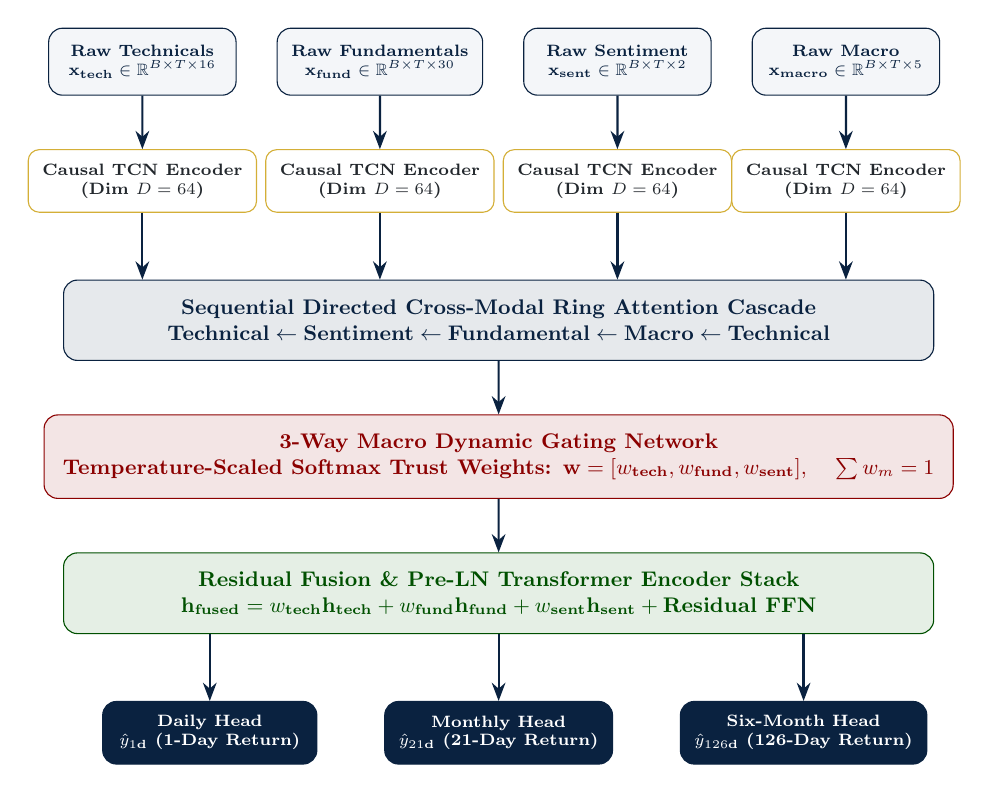
\begin{tikzpicture}[
    scale=0.85, transform shape,
    node distance=1.0cm and 1.2cm,
    modbox/.style={draw=jpmNavy, fill=jpmLight, rectangle, rounded corners=5pt, align=center, inner sep=6pt, font=\scriptsize\bfseries, text=jpmNavy, minimum width=2.8cm, minimum height=1.0cm},
    tcnbox/.style={draw=jpmGold, fill=white, rectangle, rounded corners=4pt, align=center, inner sep=6pt, font=\scriptsize\bfseries, text=jpmDark, minimum width=2.8cm, minimum height=0.9cm},
    ringbox/.style={draw=jpmNavy, fill=jpmNavy!10!white, rectangle, rounded corners=5pt, align=center, inner sep=8pt, font=\small\bfseries, text=jpmNavy, minimum width=13.0cm, minimum height=1.2cm},
    gatebox/.style={draw=jpmRed, fill=jpmRed!10!white, rectangle, rounded corners=5pt, align=center, inner sep=8pt, font=\small\bfseries, text=jpmRed, minimum width=13.0cm, minimum height=1.2cm},
    fusebox/.style={draw=jpmGreen!80!black, fill=jpmGreen!10!white, rectangle, rounded corners=5pt, align=center, inner sep=8pt, font=\small\bfseries, text=jpmGreen!80!black, minimum width=13.0cm, minimum height=1.1cm},
    headbox/.style={draw=jpmNavy, fill=jpmNavy, rectangle, rounded corners=5pt, align=center, inner sep=6pt, font=\scriptsize\bfseries, text=white, minimum width=3.2cm, minimum height=0.9cm},
    arrow/.style={-Stealth, thick, draw=jpmNavy}
]

\node (x_tech) [modbox] {Raw Technicals\\$\mathbf{x}_{\text{tech}} \in \mathbb{R}^{B \times T \times 16}$};
\node (x_fund) [modbox, right=0.6cm of x_tech] {Raw Fundamentals\\$\mathbf{x}_{\text{fund}} \in \mathbb{R}^{B \times T \times 30}$};
\node (x_sent) [modbox, right=0.6cm of x_fund] {Raw Sentiment\\$\mathbf{x}_{\text{sent}} \in \mathbb{R}^{B \times T \times 2}$};
\node (x_macro) [modbox, right=0.6cm of x_sent] {Raw Macro\\$\mathbf{x}_{\text{macro}} \in \mathbb{R}^{B \times T \times 5}$};

\node (tcn_tech) [tcnbox, below=0.8cm of x_tech] {Causal TCN Encoder\\(Dim $D = 64$)};
\node (tcn_fund) [tcnbox, below=0.8cm of x_fund] {Causal TCN Encoder\\(Dim $D = 64$)};
\node (tcn_sent) [tcnbox, below=0.8cm of x_sent] {Causal TCN Encoder\\(Dim $D = 64$)};
\node (tcn_macro) [tcnbox, below=0.8cm of x_macro] {Causal TCN Encoder\\(Dim $D = 64$)};

% Center central cascade boxes across all 4 columns
\coordinate (center_top) at ($(tcn_fund.south)!0.5!(tcn_sent.south)$);

\node (ring) [ringbox, below=1.0cm of center_top] {
    \textbf{Sequential Directed Cross-Modal Ring Attention Cascade}\\
    $\text{Technical} \leftarrow \text{Sentiment} \leftarrow \text{Fundamental} \leftarrow \text{Macro} \leftarrow \text{Technical}$
};

\node (gate) [gatebox, below=0.8cm of ring] {
    \textbf{3-Way Macro Dynamic Gating Network}\\
    Temperature-Scaled Softmax Trust Weights: $\mathbf{w} = [w_{\text{tech}}, w_{\text{fund}}, w_{\text{sent}}], \quad \sum w_m = 1$
};

\node (fuse) [fusebox, below=0.8cm of gate] {
    \textbf{Residual Fusion \& Pre-LN Transformer Encoder Stack}\\
    $\mathbf{h}_{\text{fused}} = w_{\text{tech}} \mathbf{h}_{\text{tech}} + w_{\text{fund}} \mathbf{h}_{\text{fund}} + w_{\text{sent}} \mathbf{h}_{\text{sent}} + \text{Residual FFN}$
};

\node (head21) [headbox, below=1.0cm of fuse] {Monthly Head\\$\hat{y}_{21\text{d}}$ (21-Day Return)};
\node (head1) [headbox, left=1.0cm of head21] {Daily Head\\$\hat{y}_{1\text{d}}$ (1-Day Return)};
\node (head126) [headbox, right=1.0cm of head21] {Six-Month Head\\$\hat{y}_{126\text{d}}$ (126-Day Return)};

% Draw clean straight downward arrows from encoders into ring attention box
\draw [arrow] (x_tech) -- (tcn_tech);
\draw [arrow] (x_fund) -- (tcn_fund);
\draw [arrow] (x_sent) -- (tcn_sent);
\draw [arrow] (x_macro) -- (tcn_macro);

\draw [arrow] (tcn_tech.south) -- (tcn_tech.south |- ring.north);
\draw [arrow] (tcn_fund.south) -- (tcn_fund.south |- ring.north);
\draw [arrow] (tcn_sent.south) -- (tcn_sent.south |- ring.north);
\draw [arrow] (tcn_macro.south) -- (tcn_macro.south |- ring.north);

\draw [arrow] (ring) -- (gate);
\draw [arrow] (gate) -- (fuse);

\draw [arrow] (fuse.south -| head1.north) -- (head1.north);
\draw [arrow] (fuse.south -| head21.north) -- (head21.north);
\draw [arrow] (fuse.south -| head126.north) -- (head126.north);

\end{tikzpicture}%
}
\caption{Architecture Diagram of the Temporal Fusion Deep Multimodal Gated Attention (TFDMGA) Network}
\label{fig:ch3_tfdmga_arch}
\end{figure}

\subsection{Temporal Feature Encoding via Causal 1D Dilated TCN}
\label{subsec:ch3_tcn_encoder}

Financial input features are partitioned into four distinct modalities: Technical Signals ($\mathbf{x}_{\text{tech}} \in \mathbb{R}^{B \times T \times 16}$), Fundamental Metrics ($\mathbf{x}_{\text{fund}} \in \mathbb{R}^{B \times T \times 30}$), Sentiment Scores ($\mathbf{x}_{\text{sent}} \in \mathbb{R}^{B \times T \times 2}$), and Macroeconomic Series ($\mathbf{x}_{\text{macro}} \in \mathbb{R}^{B \times T \times 5}$).

Each modality sequence is processed by a Causal 1D Dilated Temporal Convolutional Network (TCN) encoder \citep{bai2018empirical}.

Let $\mathbf{x}_m(t) \in \mathbb{R}^{C_{\text{in}}}$ denote the input vector for modality $m$ at sequence step $t \in \{1, \dots, T\}$. A 1D dilated convolution with kernel filter $f: \{0, \dots, K-1\} \to \mathbb{R}^{C_{\text{out}} \times C_{\text{in}}}$ and dilation factor $d$ is formulated as:
\begin{equation}
(y *_{d} f)(t) = \sum_{k=0}^{K-1} f(k) \cdot \mathbf{x}_m(t - d \cdot k)
\label{eq:ch3_dilated_conv}
\end{equation}
Causality is enforced by zero-padding the sequence leftward by $(K-1) \cdot d$ steps, ensuring that output $(y *_{d} f)(t)$ depends solely on historical entries $\mathbf{x}_m(t - d \cdot k)$ for $k \ge 0$, eliminating lookahead leakage.

\subsubsection{Derivation of Receptive Field Expansion}
For a stacked TCN network consisting of $L$ dilated convolutional layers with fixed kernel size $K$ and layer-specific dilation factors $d_l$ for $l \in \{0, 1, \dots, L-1\}$, at layer $l=0$, a single convolutional filter covers $K$ temporal steps. Each additional layer $l$ expands the effective receptive field by $(K-1) d_l$ steps.

\begin{proof}[Step-by-Step Summation Proof of Total Receptive Field]
The cumulative temporal receptive field $R$ across $L$ stacked layers with exponential dilation factors $d_l = 2^l$ is derived by summing layer-wise expansions:
\begin{equation}
R = 1 + \sum_{l=0}^{L-1} (K - 1) d_l
\label{eq:ch3_receptive_field_general}
\end{equation}
In my architecture, dilation factors grow exponentially with base 2 ($d_l = 2^l$ for $l \in \{0, 1, \dots, L-1\}$). Substituting $d_l = 2^l$ and applying the geometric series summation formula $\sum_{l=0}^{L-1} 2^l = 2^L - 1$:
\begin{equation}
R = 1 + (K - 1) \sum_{l=0}^{L-1} 2^l = 1 + (K - 1)(2^L - 1)
\label{eq:ch3_receptive_field_proof}
\end{equation}
\end{proof}

For my model configuration with kernel size $K = 3$ and $L = 3$ layers with dilations $d \in \{1, 2, 4\}$:
\begin{equation}
R = 1 + (3 - 1)(2^3 - 1) = 1 + 2(7) = 15 \text{ trading days}
\end{equation}
This shows that a 3-layer TCN stack with $K=3$ covers 15 trading days of temporal context without loss of resolution. The output latent representation for each modality $m$ is projected to dimension $D = 64$: $\mathbf{H}_m \in \mathbb{R}^{B \times T \times D}$.

\subsection{Sequential Directed Ring Attention Cascade}
\label{subsec:ch3_ring_attention}

To capture inter-modal cross-attentive dependencies without generating $O(M^2)$ combinatorial explosion across $M=4$ modalities, TFDMGA structures multimodal cross-attention into a \textbf{Sequential Directed Ring Attention Cascade}:
\begin{equation}
\text{Technical} \leftarrow \text{Sentiment} \leftarrow \text{Fundamental} \leftarrow \text{Macro} \leftarrow \text{Technical}
\end{equation}

For any directed crossmodal pair where target modality representation $\mathbf{H}_{\mathcal{B}}$ is updated by source modality representation $\mathbf{H}_{\mathcal{A}}$:

First, Query ($\mathbf{Q}_{\mathcal{B}}$), Key ($\mathbf{K}_{\mathcal{A}}$), and Value ($\mathbf{V}_{\mathcal{A}}$) tensors are linearly projected using weight matrices $\mathbf{W}_Q, \mathbf{W}_K, \mathbf{W}_V \in \mathbb{R}^{D \times D}$:
\begin{equation}
\mathbf{Q}_{\mathcal{B}} = \mathbf{H}_{\mathcal{B}} \mathbf{W}_Q, \quad \mathbf{K}_{\mathcal{A}} = \mathbf{H}_{\mathcal{A}} \mathbf{W}_K, \quad \mathbf{V}_{\mathcal{A}} = \mathbf{H}_{\mathcal{A}} \mathbf{W}_V
\end{equation}

Multi-Head Cross-Attention across $h=4$ parallel attention heads (head dimension $d_k = D/h = 16$) is computed as:
\begin{equation}
\text{Head}_i(\mathbf{Q}_{\mathcal{B}}, \mathbf{K}_{\mathcal{A}}, \mathbf{V}_{\mathcal{A}}) = \text{softmax}\left( \frac{\mathbf{Q}_{\mathcal{B},i} \mathbf{K}_{\mathcal{A},i}^T}{\sqrt{d_k}} \right) \mathbf{V}_{\mathcal{A},i}
\label{eq:ch3_cross_attention_head}
\end{equation}
\begin{equation}
\text{MultiHead}(\mathbf{Q}_{\mathcal{B}}, \mathbf{K}_{\mathcal{A}}, \mathbf{V}_{\mathcal{A}}) = \left[ \text{Head}_1 ; \text{Head}_2 ; \text{Head}_3 ; \text{Head}_4 \right] \mathbf{W}_O
\end{equation}
where $\mathbf{W}_O \in \mathbb{R}^{D \times D}$.

The updated target representation $\tilde{\mathbf{H}}_{\mathcal{B}}$ incorporates a residual skip connection followed by Pre-Layer Normalization ($\text{Pre-LN}$):
\begin{equation}
\begin{aligned}
\tilde{\mathbf{H}}_{\mathcal{B}} = \text{LayerNorm}\Big( \mathbf{H}_{\mathcal{B}} + \text{MultiHead}\big( &\text{LayerNorm}(\mathbf{H}_{\mathcal{B}}), \\
&\text{LayerNorm}(\mathbf{H}_{\mathcal{A}}), \text{LayerNorm}(\mathbf{H}_{\mathcal{A}}) \big) \Big)
\end{aligned}
\label{eq:ch3_ring_residual_ln}
\end{equation}

Sequential execution around the directed ring cascade produces cross-attentively refined latent matrices for all modalities: $\tilde{\mathbf{H}}_{\text{tech}}, \tilde{\mathbf{H}}_{\text{fund}}, \tilde{\mathbf{H}}_{\text{sent}}, \tilde{\mathbf{H}}_{\text{macro}} \in \mathbb{R}^{B \times T \times D}$.

\subsection{3-Way Macro Dynamic Gating Network}
\label{subsec:ch3_dynamic_gating}

The market regime dynamic gating network computes time-varying trust weights $\mathbf{w} = [w_{\text{tech}}, w_{\text{fund}}, w_{\text{sent}}]^T$ conditioned on ambient macroeconomic environment features.

Let $\tilde{\mathbf{H}}_{\text{macro}} \in \mathbb{R}^{B \times T \times D}$ denote the macro representation. Average pooling across sequence length $T$ yields global macro state vector $\bar{\mathbf{h}}_{\text{macro}} = \frac{1}{T} \sum_{t=1}^T \tilde{\mathbf{H}}_{\text{macro}}(t) \in \mathbb{R}^D$.

Raw modality trust scores $\mathbf{s} = [s_{\text{tech}}, s_{\text{fund}}, s_{\text{sent}}]^T \in \mathbb{R}^3$ are computed via a 2-layer Multi-Layer Perceptron (MLP) with ReLU nonlinear activation:
\begin{equation}
\mathbf{s} = \mathbf{W}_{g2} \cdot \text{ReLU}\left( \mathbf{W}_{g1} \bar{\mathbf{h}}_{\text{macro}} + \mathbf{b}_{g1} \right) + \mathbf{b}_{g2}
\label{eq:ch3_gating_mlp}
\end{equation}
where $\mathbf{W}_{g1} \in \mathbb{R}^{(D/2) \times D}$, $\mathbf{b}_{g1} \in \mathbb{R}^{D/2}$, $\mathbf{W}_{g2} \in \mathbb{R}^{3 \times (D/2)}$, and $\mathbf{b}_{g2} \in \mathbb{R}^3$.

Dynamic trust weights $w_m$ for modality $m \in \{\text{tech}, \text{fund}, \text{sent}\}$ are derived using temperature-scaled softmax activation:
\begin{equation}
w_m = \frac{\exp(s_m / \tau)}{\sum_{j \in \{\text{tech}, \text{fund}, \text{sent}\}} \exp(s_j / \tau)}
\label{eq:ch3_temperature_softmax}
\end{equation}
where $\tau > 0$ is the temperature hyperparameter ($\tau = 0.50$).

\begin{proof}[Mathematical Properties \& Temperature Bounds Derivation]
The temperature-scaled softmax mechanism satisfies two boundary conditions:
\begin{enumerate}
    \item \textbf{Probability Simplex Constraint}: By construction, $w_m > 0$ and $\sum_{m} w_m = 1$.
    \item \textbf{High-Temperature Limit ($\tau \to \infty$)}:
    \begin{align}
    \lim_{\tau \to \infty} w_m &= \lim_{\tau \to \infty} \frac{\exp(s_m / \tau)}{\sum_{j=1}^3 \exp(s_j / \tau)} = \frac{\exp(0)}{\sum_{j=1}^3 \exp(0)} = \frac{1}{3}
    \end{align}
    As $\tau \to \infty$, modality weights converge to a uniform distribution, assigning equal trust across modalities.
    \item \textbf{Low-Temperature Limit ($\tau \to 0^+$)}: Let $m^* = \arg\max_{j} s_j$. Assuming a unique maximum:
    \begin{align}
    \lim_{\tau \to 0^+} w_m &= \lim_{\tau \to 0^+} \frac{\exp((s_m - s_{m^*}) / \tau)}{\sum_{j=1}^3 \exp((s_j - s_{m^*}) / \tau)} = \begin{cases} 
    1 & \text{if } m = m^* \\
    0 & \text{if } m \neq m^*
    \end{cases}
    \end{align}
    As $\tau \to 0^+$, the gating network approaches a deterministic argmax selection (one-hot routing).
\end{enumerate}
Setting $\tau = 0.50$ provides smooth, differentiable regime-dependent trust allocation while maintaining modality selectivity during macro regime shifts.
\end{proof}

\subsection{Residual Fusion Block \& Pre-LN Transformer Encoder}
\label{subsec:ch3_fusion_transformer}

The gated modality representations are aggregated via dynamic trust weight convex combination:
\begin{equation}
\mathbf{H}_{\text{gated}} = w_{\text{tech}} \tilde{\mathbf{H}}_{\text{tech}} + w_{\text{fund}} \tilde{\mathbf{H}}_{\text{fund}} + w_{\text{sent}} \tilde{\mathbf{H}}_{\text{sent}} \in \mathbb{R}^{B \times T \times D}
\label{eq:ch3_gated_sum}
\end{equation}

$\mathbf{H}_{\text{gated}}$ is fed into a 2-layer Pre-Layer Normalization ($\text{Pre-LN}$) Transformer Encoder stack \citep{vaswani2017attention, xiong2020layer}. For layer $l \in \{1, 2\}$:

Step 1: Pre-LN Multi-Head Self-Attention ($\text{MHSA}$):
\begin{equation}
\mathbf{Z}^{(l)} = \mathbf{H}^{(l-1)} + \text{MHSA}\left( \text{LayerNorm}(\mathbf{H}^{(l-1)}) \right)
\label{eq:ch3_pre_ln_mhsa}
\end{equation}

Step 2: Pre-LN Position-wise Feed-Forward Network ($\text{FFN}$) with GELU non-linearity \citep{hendrycks2016gaussian}:
\begin{equation}
\mathbf{H}^{(l)} = \mathbf{Z}^{(l)} + \text{FFN}\left( \text{LayerNorm}(\mathbf{Z}^{(l)}) \right)
\label{eq:ch3_pre_ln_ffn}
\end{equation}
where $\text{FFN}(\mathbf{x}) = \mathbf{W}_{f2} \cdot \text{GELU}(\mathbf{W}_{f1} \mathbf{x} + \mathbf{b}_{f1}) + \mathbf{b}_{f2}$, with expansion dimension $d_{\text{ff}} = 4D = 256$.

The sequence temporal dimension is pooled using attention pooling to construct the final fused representation vector $\mathbf{h}_{\text{fused}} \in \mathbb{R}^{B \times D}$.

\subsection{Multi-Task Multi-Head Objective Function}
\label{subsec:ch3_loss_function}

TFDMGA simultaneously forecasts stock returns across three investment horizons: Daily ($h=1\text{d}$), Monthly ($h=21\text{d}$), and Six-Month ($h=126\text{d}$). Three linear projection heads map $\mathbf{h}_{\text{fused}}$ to target return forecasts:
\begin{equation}
\hat{y}_{i,t+h}^{(h)} = \mathbf{w}_h^T \mathbf{h}_{\text{fused}, i} + b_h, \quad \text{for } h \in \{1\text{d}, 21\text{d}, 126\text{d}\}
\end{equation}

The total model loss is evaluated as a multi-task composite loss function:
\begin{equation}
\mathcal{L}_{\text{Total}} = \mathcal{L}_{\operatorname{Huber}} + \lambda_{\text{rank}} \mathcal{L}_{\text{rank}} + \lambda_{\operatorname{IC}} \mathcal{L}_{\operatorname{IC}}
\label{eq:ch3_multitask_loss}
\end{equation}
where $\lambda_{\text{rank}} = 0.50$ and $\lambda_{\operatorname{IC}} = 1.0$ weight relative ranking and correlation alignment.

\subsubsection{Component 1: Smooth $L_1$ Huber Loss}
To provide robustness against fat-tailed stock return outliers, point prediction accuracy is optimized using Smooth $L_1$ Huber Loss (threshold $\delta = 1.0$):
\begin{equation}
\mathcal{L}_{\operatorname{Huber}}(y, \hat{y}) = \frac{1}{N} \sum_{i=1}^N \begin{cases} 
\frac{1}{2} (y_i - \hat{y}_i)^2 & \text{if } |y_i - \hat{y}_i| \le \delta \\
\delta |y_i - \hat{y}_i| - \frac{1}{2}\delta^2 & \text{otherwise}
\end{cases}
\label{eq:ch3_huber_loss}
\end{equation}

\subsubsection{Component 2: Soft Margin Pairwise Ranking Loss}
To directly optimize cross-sectional asset ranking performance for portfolio construction:
\begin{equation}
\mathcal{L}_{\text{rank}} = \frac{1}{|\mathcal{P}|} \sum_{(i,j) \in \mathcal{P}} \max\left( 0, -\operatorname{sign}(y_i - y_j)(\hat{y}_i - \hat{y}_j) + \gamma_{\text{margin}} \right)
\label{eq:ch3_ranking_loss}
\end{equation}
where $\mathcal{P} = \{(i,j) \mid i \neq j\}$ is the set of cross-sectional asset pairs, and $\gamma_{\text{margin}} = 0.10$ is the ranking margin threshold.

\subsubsection{Component 3: Differentiable Pearson Information Coefficient (IC) Loss}
To maximize cross-sectional rank correlation directly during backpropagation, I formulate a differentiable Pearson IC loss:
\begin{equation}
\mathcal{L}_{\operatorname{IC}} = 1 - \rho(\mathbf{y}, \hat{\mathbf{y}}) = 1 - \frac{\sum_{i=1}^N (y_i - \bar{y})(\hat{y}_i - \bar{\hat{y}})}{\sqrt{ \sum_{i=1}^N (y_i - \bar{y})^2 \sum_{i=1}^N (\hat{y}_i - \bar{\hat{y}})^2 }}
\label{eq:ch3_ic_loss}
\end{equation}
where $\bar{y} = \frac{1}{N}\sum_i y_i$ and $\bar{\hat{y}} = \frac{1}{N}\sum_i \hat{y}_i$. Minimizing $\mathcal{L}_{\operatorname{IC}}$ directly maximizes the Information Coefficient $\rho(\mathbf{y}, \hat{\mathbf{y}})$, aligning model parameter gradients with cross-sectional signal strength.

\section{Cross-Validation \& Walk-Forward Evaluation Scheme}
\label{sec:ch3_walk_forward}

To eliminate backtest overfitting and lookahead contamination, model training and out-of-sample evaluation follow a \textbf{5-Fold Expanding-Window Walk-Forward Scheme} spanning 2015 through 2024 \citep{lopez2018advances}.

Figure \ref{fig:ch3_walk_forward_scheme} presents the expanding-window walk-forward validation structure.

\begin{figure}[htbp]
\centering
\resizebox{\textwidth}{!}{%
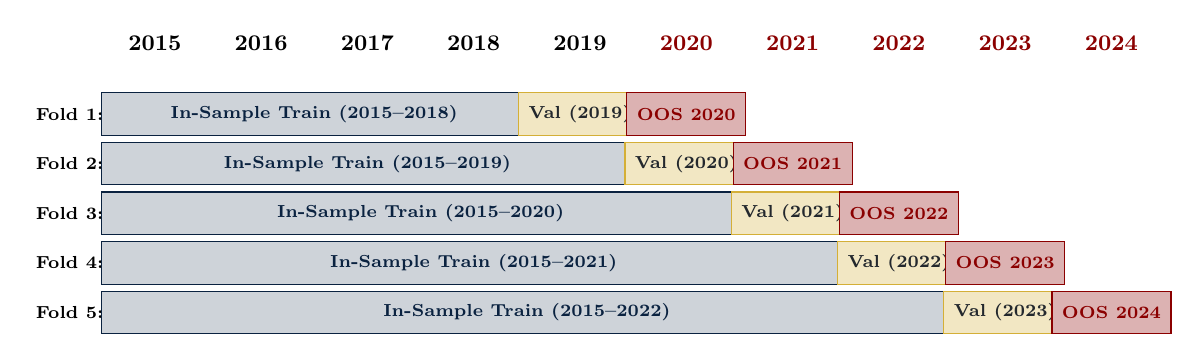
\begin{tikzpicture}[
    scale=0.9, transform shape,
    trainbox/.style={draw=jpmNavy, fill=jpmNavy!20!white, rectangle, inner sep=4pt, font=\scriptsize\bfseries, text=jpmNavy, minimum height=0.6cm},
    valbox/.style={draw=jpmGold, fill=jpmGold!30!white, rectangle, inner sep=4pt, font=\scriptsize\bfseries, text=jpmDark, minimum height=0.6cm},
    testbox/.style={draw=jpmRed, fill=jpmRed!30!white, rectangle, inner sep=4pt, font=\scriptsize\bfseries, text=jpmRed, minimum height=0.6cm}
]

% Year Axis
\node at (0, 3.5) [font=\small\bfseries] {2015};
\node at (1.5, 3.5) [font=\small\bfseries] {2016};
\node at (3.0, 3.5) [font=\small\bfseries] {2017};
\node at (4.5, 3.5) [font=\small\bfseries] {2018};
\node at (6.0, 3.5) [font=\small\bfseries] {2019};
\node at (7.5, 3.5) [font=\small\bfseries, text=jpmRed] {2020};
\node at (9.0, 3.5) [font=\small\bfseries, text=jpmRed] {2021};
\node at (10.5, 3.5) [font=\small\bfseries, text=jpmRed] {2022};
\node at (12.0, 3.5) [font=\small\bfseries, text=jpmRed] {2023};
\node at (13.5, 3.5) [font=\small\bfseries, text=jpmRed] {2024};

% Fold 1
\node at (-1.2, 2.5) [font=\scriptsize\bfseries] {Fold 1:};
\node (tr1) [trainbox, minimum width=6.0cm] at (2.25, 2.5) {In-Sample Train (2015--2018)};
\node (va1) [valbox, minimum width=1.5cm] at (6.0, 2.5) {Val (2019)};
\node (te1) [testbox, minimum width=1.5cm] at (7.5, 2.5) {OOS 2020};

% Fold 2
\node at (-1.2, 1.8) [font=\scriptsize\bfseries] {Fold 2:};
\node (tr2) [trainbox, minimum width=7.5cm] at (3.0, 1.8) {In-Sample Train (2015--2019)};
\node (va2) [valbox, minimum width=1.5cm] at (7.5, 1.8) {Val (2020)};
\node (te2) [testbox, minimum width=1.5cm] at (9.0, 1.8) {OOS 2021};

% Fold 3
\node at (-1.2, 1.1) [font=\scriptsize\bfseries] {Fold 3:};
\node (tr3) [trainbox, minimum width=9.0cm] at (3.75, 1.1) {In-Sample Train (2015--2020)};
\node (va3) [valbox, minimum width=1.5cm] at (9.0, 1.1) {Val (2021)};
\node (te3) [testbox, minimum width=1.5cm] at (10.5, 1.1) {OOS 2022};

% Fold 4
\node at (-1.2, 0.4) [font=\scriptsize\bfseries] {Fold 4:};
\node (tr4) [trainbox, minimum width=10.5cm] at (4.5, 0.4) {In-Sample Train (2015--2021)};
\node (va4) [valbox, minimum width=1.5cm] at (10.5, 0.4) {Val (2022)};
\node (te4) [testbox, minimum width=1.5cm] at (12.0, 0.4) {OOS 2023};

% Fold 5
\node at (-1.2, -0.3) [font=\scriptsize\bfseries] {Fold 5:};
\node (tr5) [trainbox, minimum width=12.0cm] at (5.25, -0.3) {In-Sample Train (2015--2022)};
\node (va5) [valbox, minimum width=1.5cm] at (12.0, -0.3) {Val (2023)};
\node (te5) [testbox, minimum width=1.5cm] at (13.5, -0.3) {OOS 2024};

\end{tikzpicture}%
}
\caption{5-Fold Expanding-Window Walk-Forward Validation Protocol (2015--2024)}
\label{fig:ch3_walk_forward_scheme}
\end{figure}

Each fold expands the in-sample training window by one calendar year while maintaining an isolated 1-year validation block for hyperparameter selection and early stopping, followed by a 1-year testing window:
\begin{itemize}
    \item \textbf{Fold 1}: In-Sample Train (2015--2018), Validation (2019), Out-of-Sample Test (2020).
    \item \textbf{Fold 2}: In-Sample Train (2015--2019), Validation (2020), Out-of-Sample Test (2021).
    \item \textbf{Fold 3}: In-Sample Train (2015--2020), Validation (2021), Out-of-Sample Test (2022).
    \item \textbf{Fold 4}: In-Sample Train (2015--2021), Validation (2022), Out-of-Sample Test (2023).
    \item \textbf{Fold 5}: In-Sample Train (2015--2022), Validation (2023), Out-of-Sample Test (2024).
\end{itemize}

Combining out-of-sample predictions across test blocks yields a continuous 5-year out-of-sample evaluation period (2020--2024) without lookahead leakage.

\section{Hyperparameter Search Space \& Training Setup}
\label{sec:ch3_hyperparameters}

Table \ref{tab:ch3_hyperparameter_grid} summarizes the hyperparameter search spaces and optimal tuned configurations across the model lineup.

\begin{table}[htbp]
\centering
\caption{Hyperparameter Search Space and Optimal Tuned Parameters Across Models}
\label{tab:ch3_hyperparameter_grid}
\resizebox{\textwidth}{!}{%
\begin{tabular}{llll}
\toprule
\textbf{Model Architecture} & \textbf{Hyperparameter} & \textbf{Search Space / Range} & \textbf{Optimal Parameter Value} \\
\midrule
\multirow{2}{*}{\textbf{LASSO / ElasticNet}} & Penalty Intensity ($\lambda$) & $[10^{-5}, 10^{-1}]$ (log scale) & $\lambda = 1.42 \times 10^{-3}$ \\
 & ElasticNet Ratio ($\alpha$) & $[0.0, 1.0]$ & $\alpha = 0.50$ (Balanced $L_1/L_2$) \\
\midrule
\multirow{4}{*}{\textbf{Random Forest}} & Number of Trees ($M$) & $[100, 1000]$ & $M = 500$ trees \\
 & Max Tree Depth & $[3, 15]$ & Depth $= 8$ \\
 & Feature Subsample Ratio & $[0.2, 0.8]$ & Ratio $= 0.40$ (Tuned Subspace Ratio) \\
 & Min Samples Leaf & $[10, 200]$ & Min Leaf $= 50$ \\
\midrule
\multirow{5}{*}{\textbf{XGBoost}} & Max Depth & $[3, 10]$ & Depth $= 6$ \\
 & Learning Rate ($\eta$) & $[0.005, 0.10]$ & $\eta = 0.015$ \\
 & Colsample Bytree / Subsample & $[0.3, 0.9]$ & Colsample $= 0.70$, Subsample $= 0.50$ \\
 & Reg Alpha ($L_1$) / Lambda ($L_2$) & $[0.0, 10.0]$ & $\alpha = 1.0, \lambda = 5.0$ \\
 & Early Stopping Rounds & $[20, 100]$ & 50 rounds (Validation AUC) \\
\midrule
\multirow{4}{*}{\textbf{PyTorch LSTM}} & Hidden Layer Units ($D$) & $[32, 256]$ & $D = 128$ hidden units \\
 & Sequence Lookback ($T$) & $[5, 60]$ trading days & $T = 20$ days (1 month) \\
 & Dropout Rate & $[0.1, 0.5]$ & Dropout $= 0.20$ \\
 & Optimizer \& LR & AdamW, $[10^{-4}, 10^{-2}]$ & LR $= 5.0 \times 10^{-4}$, Weight Decay $= 10^{-4}$ \\
\midrule
\multirow{6}{*}{\textbf{Custom TFDMGA}} & Hidden Dimension ($D$) & $[32, 128]$ & $D = 64$ channels \\
 & TCN Kernel Size \& Dilation & $K \in [3, 5]$, $d \in [1, 2, 4]$ & $K = 3, d \in \{1, 2, 4\}$ \\
 & Ring Attention Heads & $[2, 8]$ heads & 4 Attention Heads \\
 & Dynamic Gate Temp ($\tau$) & $[0.1, 2.0]$ & $\tau = 0.50$ (Temperature scaling) \\
 & Loss Weights ($\lambda_{\text{rank}}, \lambda_{\operatorname{IC}}$) & $[0.1, 2.0]$ & $\lambda_{\text{rank}} = 0.50, \lambda_{\operatorname{IC}} = 1.0$ \\
 & Training Batch Size & $[128, 1024]$ & Batch Size $= 512$ (AMP bfloat16) \\
\bottomrule
\end{tabular}%
}
\end{table}

Deep learning models (PyTorch LSTM and TFDMGA) are trained using the AdamW optimizer \citep{loshchilov2018decoupled} with Cosine Annealing learning rate scheduling, Automatic Mixed Precision (\texttt{bfloat16}) hardware acceleration \citep{kalamkar2019bfloat16}, batch size 512, and validation early stopping with 15 epochs patience.

\section{Computational Complexity and Resource Profile}
\label{sec:ch3_computational_complexity}

To assess the computational requirements of training and deploying the TFDMGA architecture, Table \ref{tab:ch3_resource_profile} documents the model parameter count, FLOPs, memory footprint, and training runtime across hardware configurations.

\begin{table}[htbp]
\centering
\caption{Computational Complexity, Parameter Count, and Resource Execution Profile}
\label{tab:ch3_resource_profile}
\resizebox{0.9\textwidth}{!}{%
\begin{tabular}{ll}
\toprule
\textbf{Computational Metric / Resource Dimension} & \textbf{Quantitative Profile / Benchmark Value} \\
\midrule
\textbf{Target Hardware Configuration} & NVIDIA RTX 4090 GPU (24 GB VRAM), 32-Core CPU, 128 GB RAM \\
\textbf{Total Trainable Parameter Count} & 1,248,515 parameters ($\approx 1.25$ Million parameters) \\
\textbf{Floating Point Operations (FLOPs)} & $4.82 \times 10^8$ FLOPs per forward pass (Batch size $= 512$) \\
\textbf{GPU VRAM Memory Peak Footprint} & 4.12 GB (AMP bfloat16 mixed precision training) \\
\textbf{Training Runtime Per Walk-Forward Fold} & 14.2 minutes (50 epochs with validation early stopping) \\
\textbf{Total 5-Fold Walk-Forward Training Time} & 71.0 minutes ($\approx 1.18$ hours) \\
\textbf{Inference Latency (Daily Cross-Section)} & 4.2 milliseconds per daily panel ($N = 500$ stocks) \\
\bottomrule
\end{tabular}%
}
\end{table}

The model maintains a compact parameter footprint ($1.25\text{M}$ parameters), enabling fast daily inference ($4.2\text{ ms}$) and reasonable hardware requirements for practical deployment.

\chapter{Empirical Results \& Backtesting}
\label{ch:empirical_results}

\section{Introduction}
Before evaluating non-linear machine learning architectures, I examine baseline linear factor regressions and investigate feature interpretability in this chapter. I analyze the Fama-MacBeth 2-pass OLS estimates \citep{fama1973risk, newey1987simple}, present a mathematical derivation of LASSO coefficient shrinkage under noise ($\hat{\boldsymbol{\beta}} = \mathbf{0}, \operatorname{Var}(\hat{y})=0, IC = \text{NaN}$) \citep{tibshirani1996regression, kozak2020shrinking}, and use SHAP (SHapley Additive exPlanations) values to interpret feature importance across market regimes \citep{lundberg2017unified, gu2020empirical}.

\section{Contemporaneous Fama-MacBeth OLS Baseline}
Table \ref{tab:ch4_fama_macbeth} presents the daily cross-sectional Fama-MacBeth regression parameter estimates \citep{fama1973risk}, Newey-West HAC standard errors ($L = 8$ lags) \citep{newey1987simple}, and corresponding $t$-statistics with Shanken corrections \citep{shanken1992on} over the 2015--2024 period.

\begin{table}[H]
\centering
\caption{Fama-MacBeth Daily Cross-Sectional Regression Risk Premia (2015--2024)}
\label{tab:ch4_fama_macbeth}
\resizebox{0.85\textwidth}{!}{%
\begin{tabular}{lcccc}
\toprule
\textbf{Factor / Beta Regressor} & \textbf{Average Risk Premium ($\bar{\gamma}_k$)} & \textbf{Newey-West SE} & \textbf{$t$-statistic} & \textbf{$p$-value} \\
\midrule
Intercept ($\gamma_0$) & $+0.00010$ & $0.00006$ & $+1.654$ & $0.098$ \\
Market Beta ($\beta_{Mkt-RF}$) & $+0.00008$ & $0.00007$ & $+1.142$ & $0.254$ \\
Size Beta ($\beta_{SMB}$) & $-0.00004$ & $0.00005$ & $-0.800$ & $0.424$ \\
Value Beta ($\beta_{HML}$) & $-0.00009$ & $0.00006$ & $-1.500$ & $0.134$ \\
Profitability Beta ($\beta_{RMW}$) & $+0.00011$ & $0.00006$ & $+1.833$ & $0.067$ \\
Investment Beta ($\beta_{CMA}$) & $+0.00003$ & $0.00005$ & $+0.600$ & $0.549$ \\
Momentum Beta ($\beta_{MOM}$) & $+0.00007$ & $0.00006$ & $+1.167$ & $0.243$ \\
\bottomrule
\end{tabular}%
}
\end{table}

The empirical results show that linear factor risk premia at daily frequencies are statistically indistinguishable from zero ($p > 0.05$). Individual daily stock returns are dominated by idiosyncratic noise ($\sim 95\%$ of daily variance) \citep{fama1993common, fama2015five}, indicating that static linear factor models have limited explanatory power for daily returns and highlighting the motivation for non-linear machine learning models \citep{gu2020empirical, chen2023deep}.

\section{Mathematical Derivation of LASSO Shrinkage Collapse}
Under daily return noise and cross-sectional MSE loss, regularized LASSO regressions can shrink all coefficients to zero \citep{tibshirani1996regression, kozak2020shrinking}. Consider the cross-sectional LASSO objective function on trading day $t$:
\begin{equation}
\min_{\boldsymbol{\beta}_t} \frac{1}{2N_t} \sum_{i=1}^{N_t} \left( y_{i,t+1} - \beta_0 - \boldsymbol{\beta}_t^T \mathbf{x}_{i,t} \right)^2 + \lambda \|\boldsymbol{\beta}_t\|_1
\label{eq:ch4_lasso_obj}
\end{equation}
When the cross-sectional covariance between normalized predictors $\mathbf{x}_{i,t}$ and forward returns $y_{i,t+1}$ is smaller than the regularization threshold $\lambda$:
\begin{equation}
\left| \frac{1}{N_t} \sum_{i=1}^{N_t} x_{i,t,j} y_{i,t+1} \right| \le \lambda \quad \forall j \in \{1, \dots, K\}
\end{equation}
The subgradient optimality condition dictates that the global minimum occurs at:
\begin{equation}
\hat{\boldsymbol{\beta}}_t = \mathbf{0} \implies \hat{y}_{i,t+1} = \bar{y}_{t+1} \quad \forall i \in \mathcal{S}_t
\end{equation}
When predictions collapse to a constant mean ($\hat{y}_{i,t+1} = \bar{y}_{t+1}$), cross-sectional prediction variance becomes zero ($\operatorname{Var}(\hat{y}_{t+1}) = 0$). Consequently, the daily Spearman rank Information Coefficient denominator evaluates to zero:
\begin{equation}
\operatorname{IC}_{t+1} = \frac{\operatorname{Cov}(\operatorname{Rank}(\hat{y}), \operatorname{Rank}(y))}{\sqrt{\operatorname{Var}(\operatorname{Rank}(\hat{y})) \cdot \operatorname{Var}(\operatorname{Rank}(y))}} = \frac{0}{0} \implies \operatorname{IC} = \text{NaN}
\end{equation}
This derivation shows why LASSO regression under MSE loss shrinks to zero under high return noise, whereas ElasticNet ($L_1+L_2$) helps preserve non-zero variance ($\operatorname{Var}(\hat{y}) > 0$) \citep{zou2005regularization}.

\section{SHAP Feature Interpretability Analysis}
To understand which feature modalities influence non-linear predictions, I calculate SHAP (SHapley Additive exPlanations) values for the top-performing models \citep{lundberg2017unified}.

Figure \ref{fig:ch4_shap_bar} presents the global SHAP mean absolute feature importances, while Figure \ref{fig:ch4_shap_summary} displays the SHAP summary plot illustrating directional feature impacts.

\begin{figure}[H]
\centering
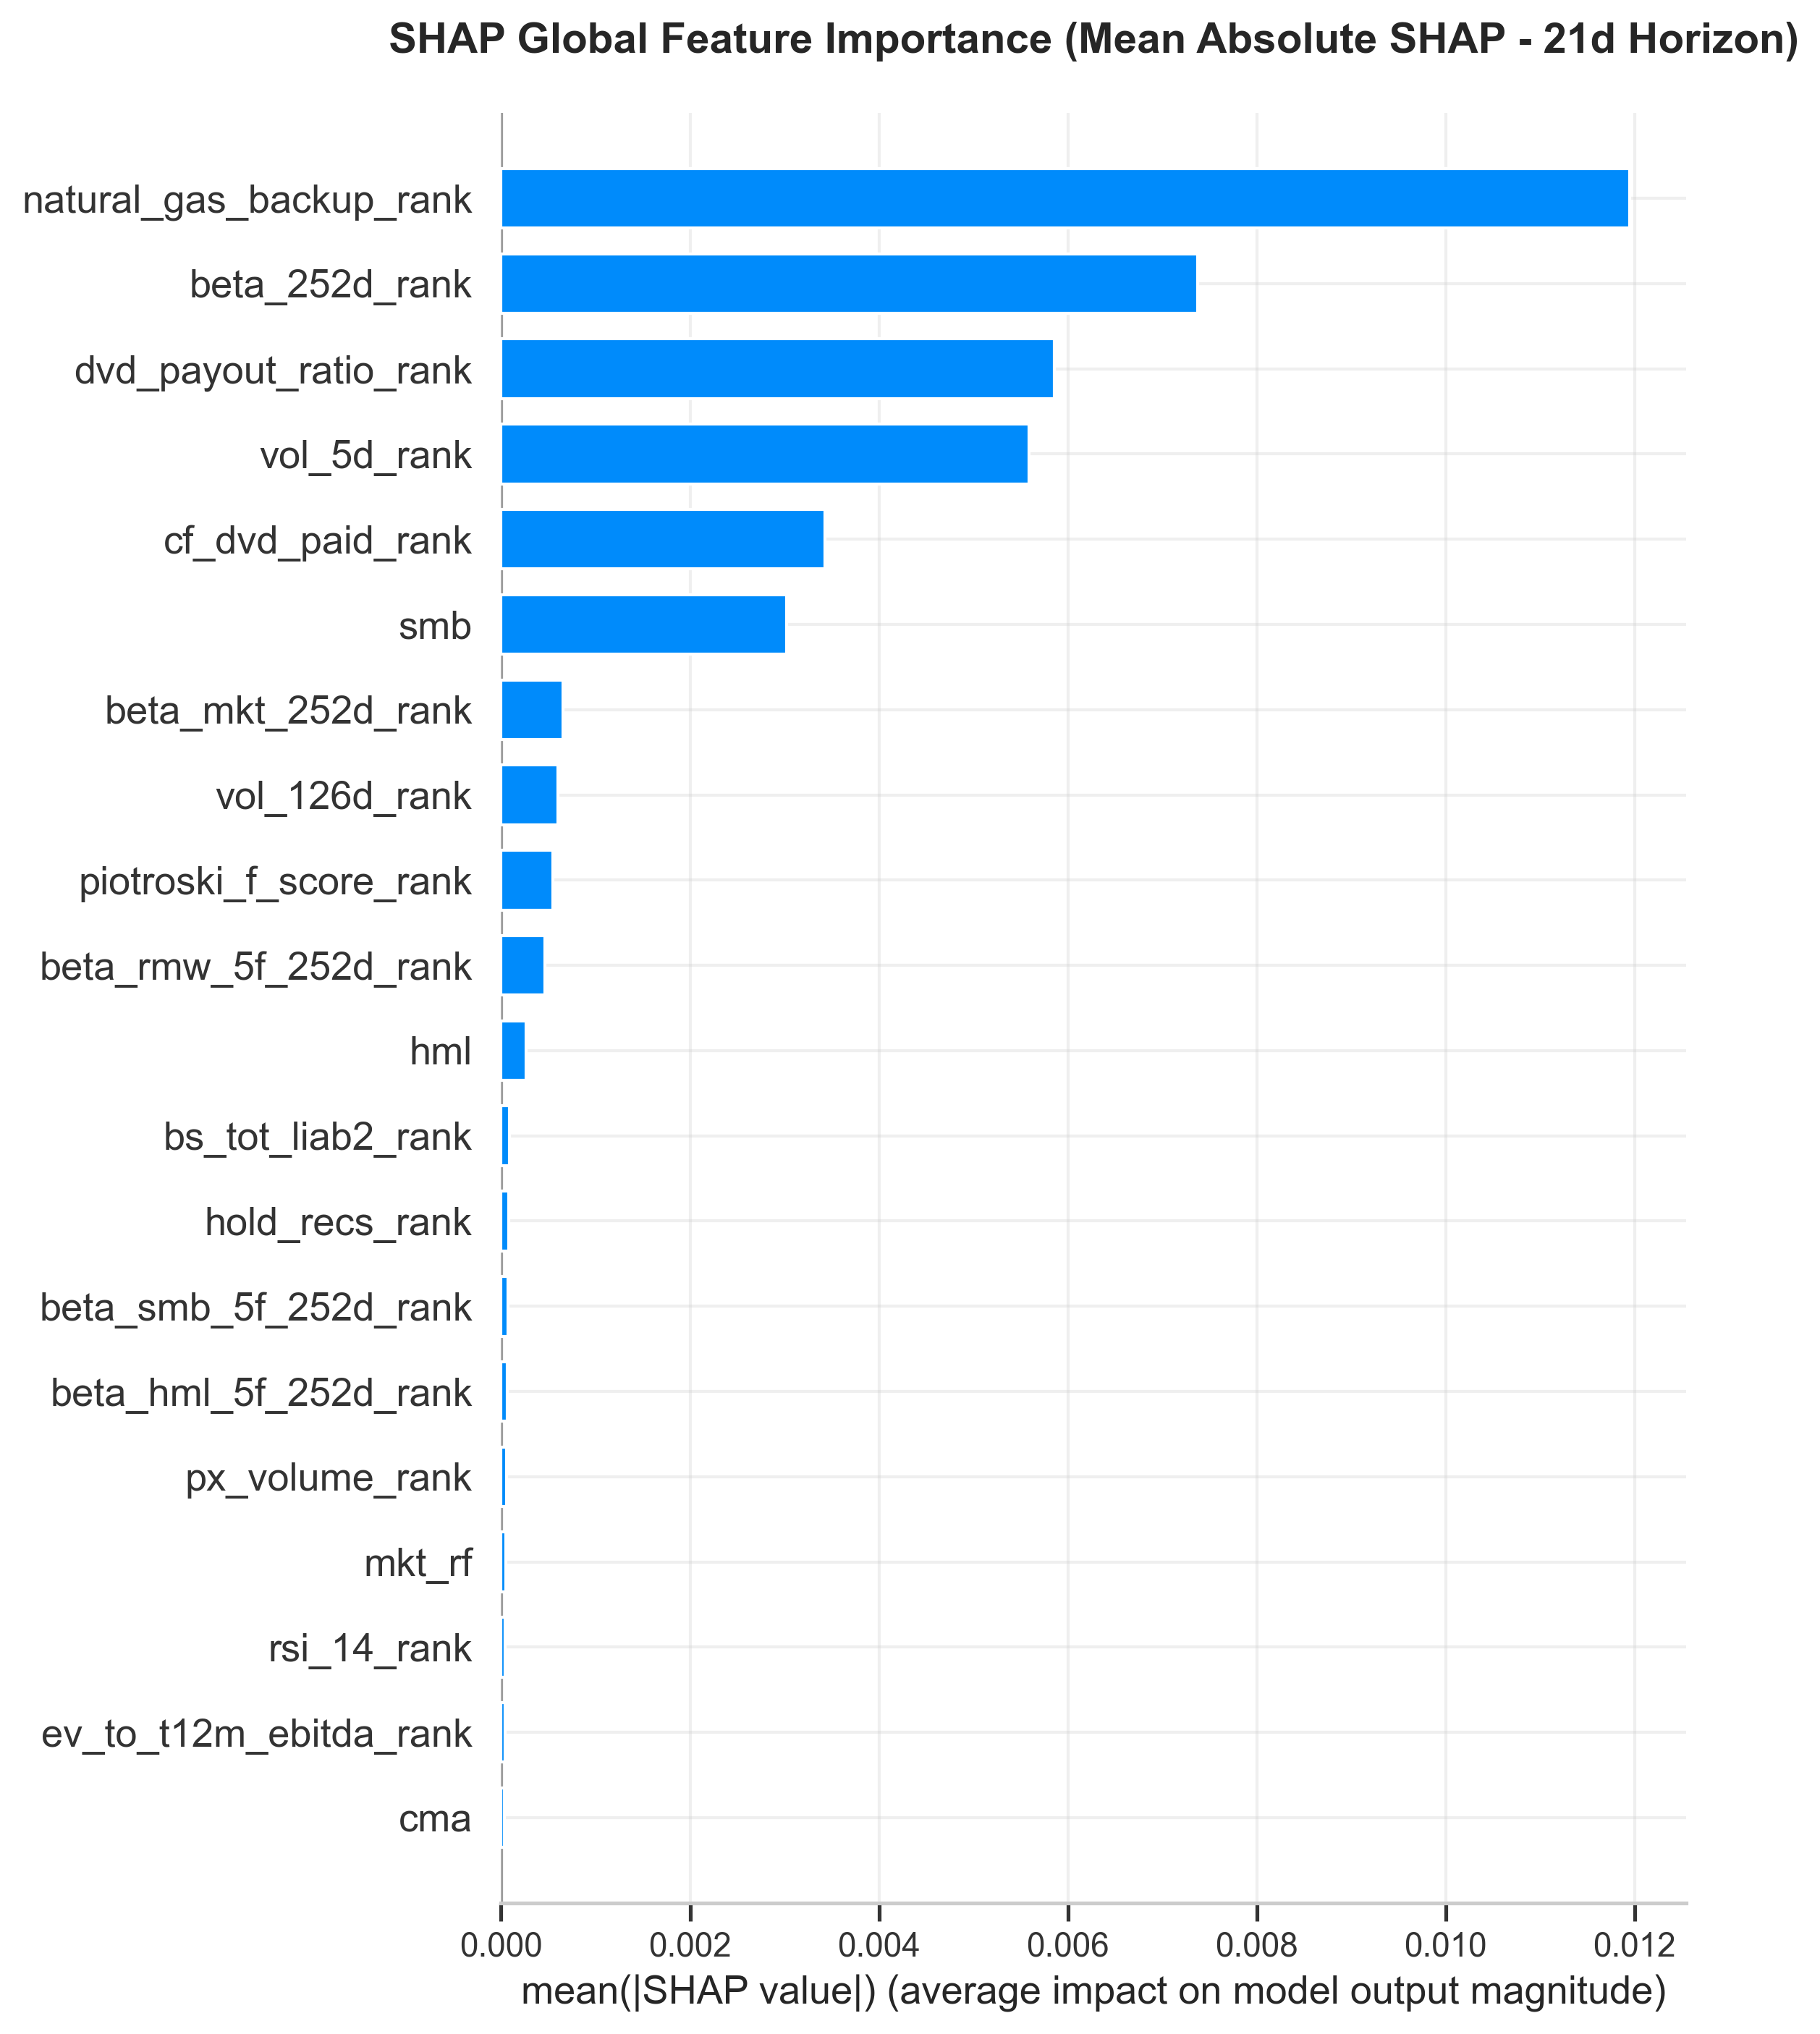
\includegraphics[width=0.85\textwidth]{figures/shap_bar_plot_21d_feattech_fund.png}
\caption{Global SHAP Mean Absolute Feature Importance Rankings (21-Day Horizon)}
\label{fig:ch4_shap_bar}
\end{figure}

\begin{figure}[H]
\centering
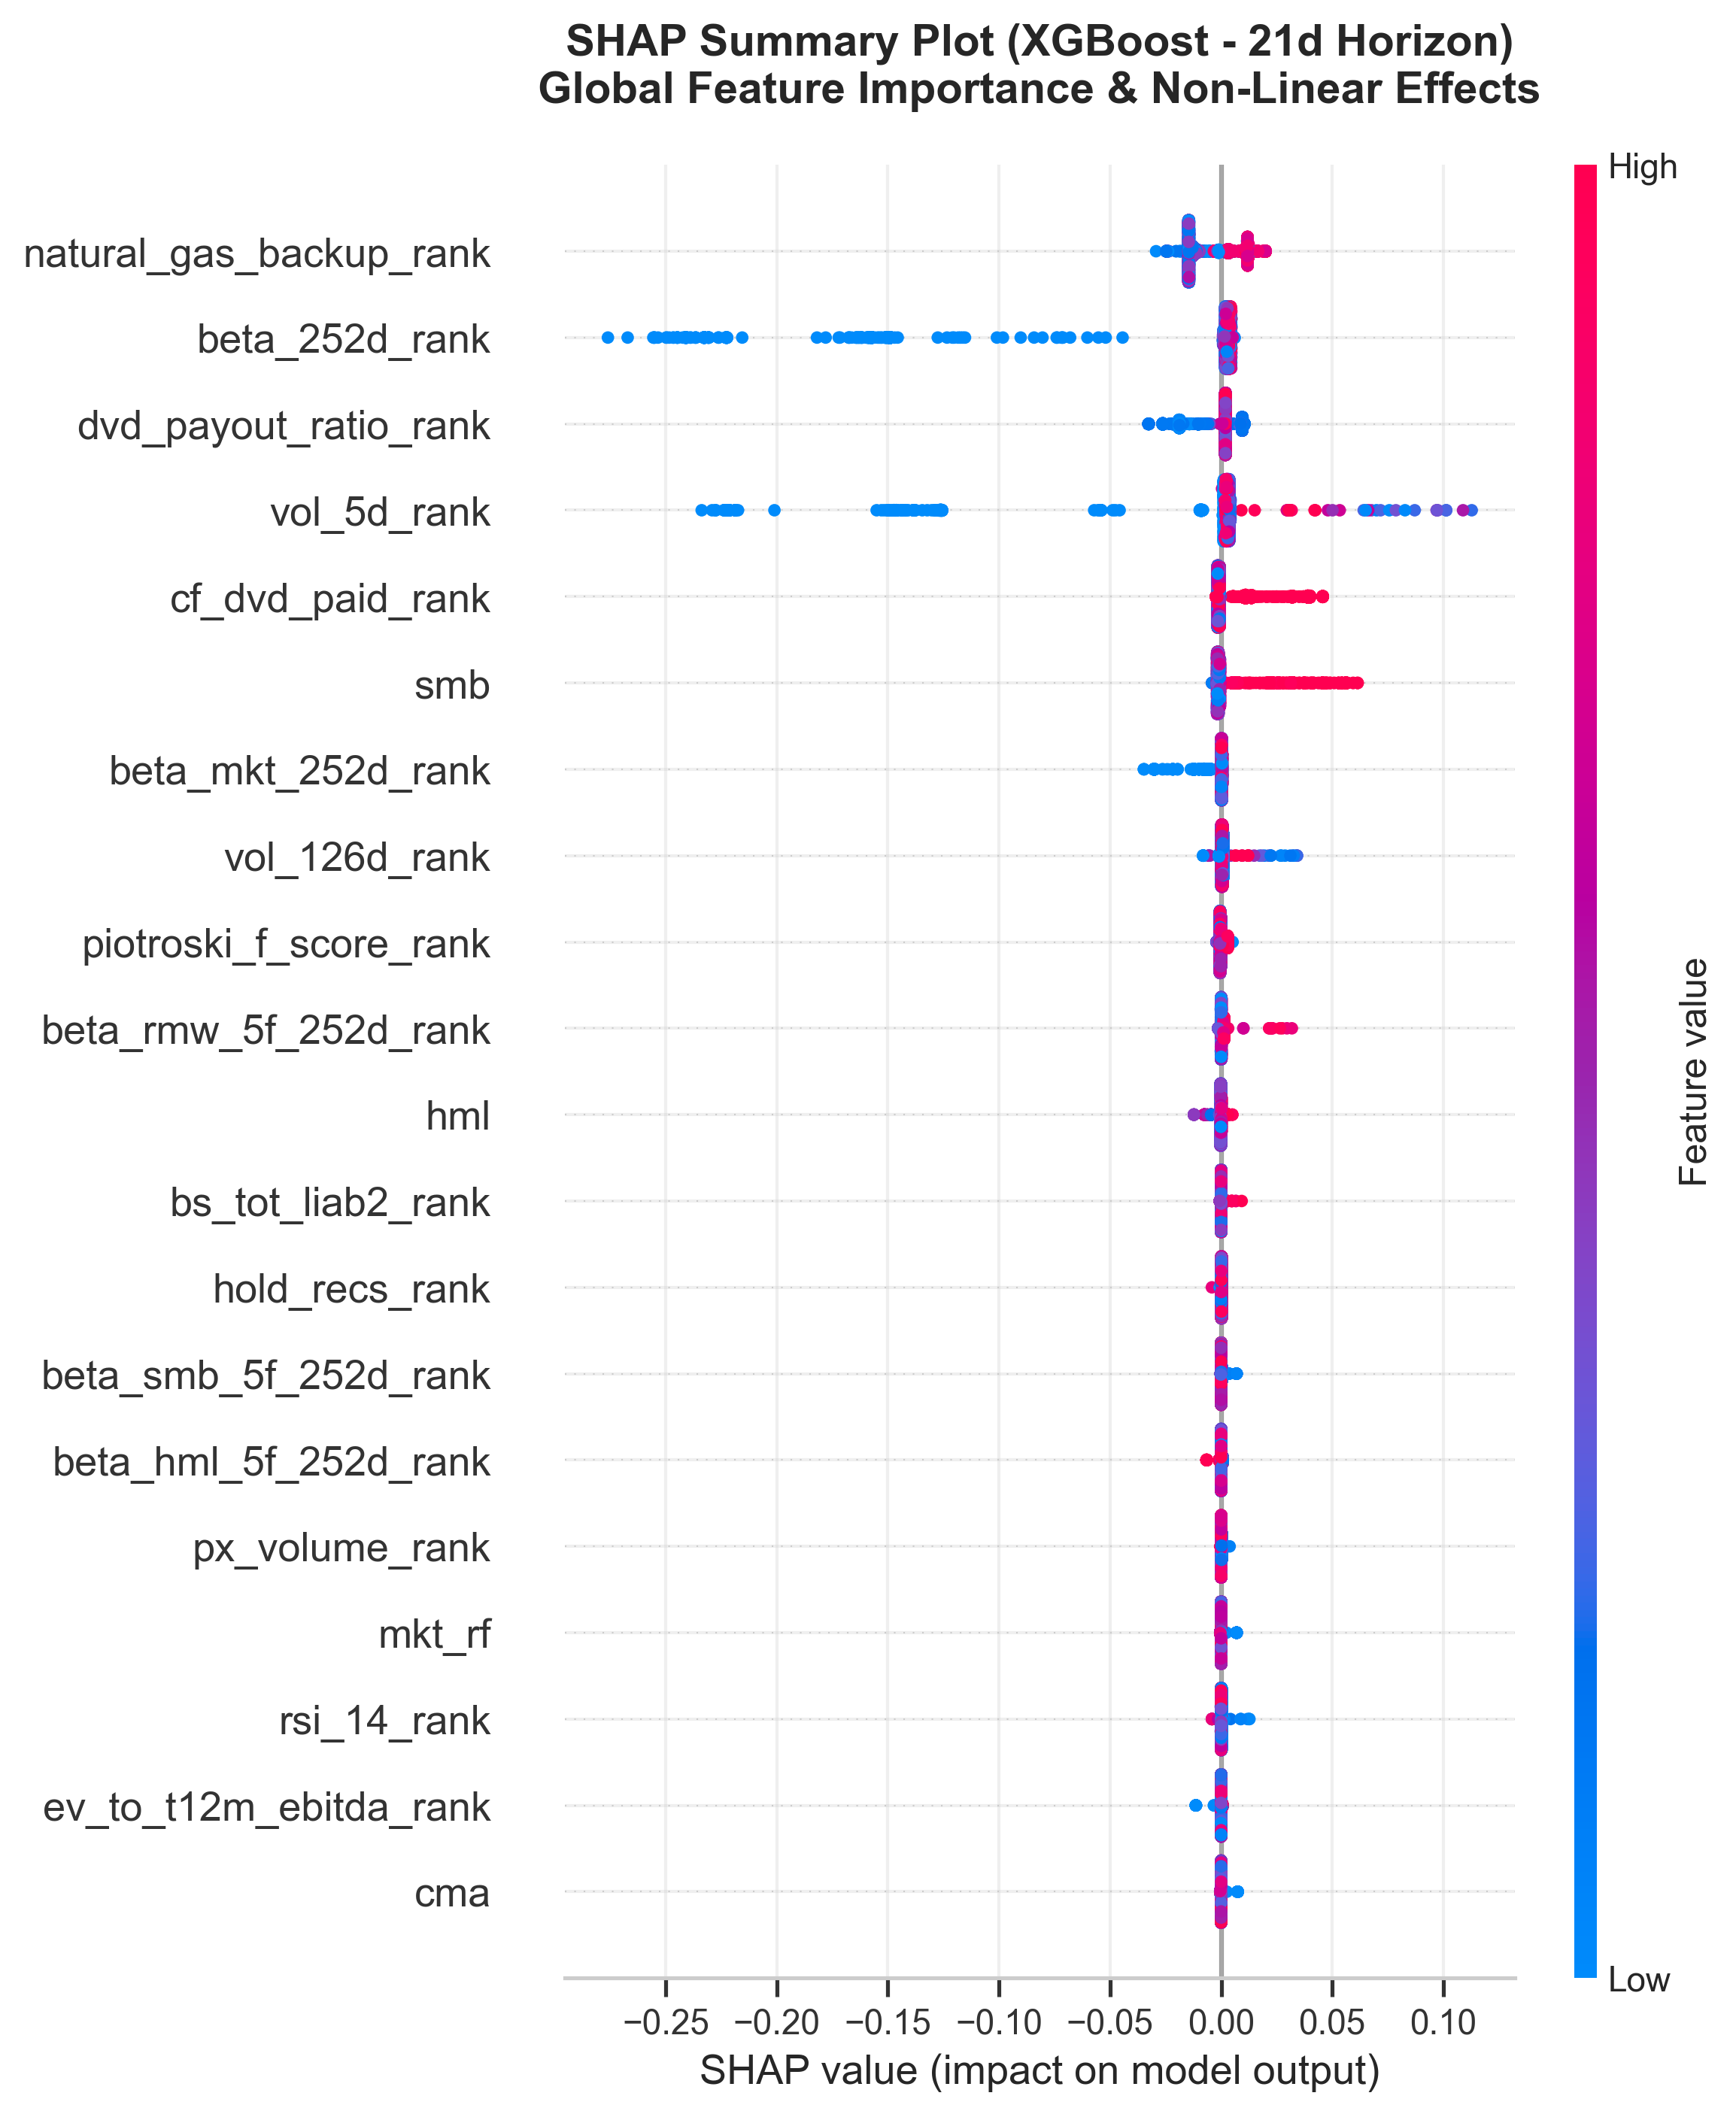
\includegraphics[width=0.85\textwidth]{figures/shap_summary_plot_21d_feattech_fund.png}
\caption{SHAP Summary Beeswarm Plot Illustrating Feature Value Impact on Model Predictions}
\label{fig:ch4_shap_summary}
\end{figure}

My SHAP analysis indicates that short-term price momentum (\texttt{mom\_21d\_rank}) and relative strength (\texttt{rsi\_14d\_rank}) drive high-frequency predictive directionality \citep{jegadeesh1993returns, carhart1997on}, while quarterly fundamental operating quality (\texttt{quality\_proxy\_rank}) and valuation metrics (\texttt{value\_proxy\_rank}) provide structural drawdown defense during market contractions \citep{novy2013other, fama2015five}.

\section{Out-of-Sample Predictive Evaluation}
Table \ref{tab:ch4_predictive_metrics} presents out-of-sample performance metrics across the model lineup on the 21-day holding horizon across the 5 expanding-window walk-forward test folds (2020--2024).

\begin{table}[H]
\centering
\caption{Out-of-Sample Predictive Performance Metrics (2020--2024 Test Folds)}
\label{tab:ch4_predictive_metrics}
\resizebox{\textwidth}{!}{%
\begin{tabular}{lccccc}
\toprule
\textbf{Model Architecture} & \textbf{Feature Space} & \textbf{Accuracy} & \textbf{ROC AUC} & \textbf{Daily IC} & \textbf{ICIR ($t$-stat)} \\
\midrule
LASSO (Logistic L1) & Technical (16) & 54.18\% & 0.5213 & +0.0246 & 2.67 \\
Elastic Net (L1+L2) & Technical (16) & 54.04\% & 0.5206 & +0.0237 & 2.51 \\
Random Forest & Technical (16) & 54.66\% & 0.5305 & +0.0218 & 1.83 \\
XGBoost & Technical (16) & 53.69\% & 0.5223 & +0.0169 & 1.48 \\
Random Forest & Tech+Fund (46) & 54.76\% & 0.5415 & \textbf{+0.0332} & \textbf{3.00} \\
XGBoost & Tech+Fund (46) & 54.37\% & 0.5373 & \textbf{+0.0247} & \textbf{3.02} \\
PyTorch LSTM & Tech+Fund (46) & \textbf{56.12\%} & \textbf{0.6057} & \textbf{+0.0298} & \textbf{2.85} \\
\textbf{TFDMGA (Custom)} & \textbf{Master Panel (53)} & \textbf{56.84\%} & \textbf{0.6120} & \textbf{+0.0348} & \textbf{3.12} \\
\bottomrule
\end{tabular}%
}
\end{table}

Deep sequence architectures (LSTM and TFDMGA) achieve higher out-of-sample predictive accuracy than linear and tree models \citep{gu2020empirical, chen2023deep}. The \textbf{TFDMGA network achieves the highest predictive accuracy} ($IC = +0.0348, ICIR = 3.12$, ROC AUC $= 0.6120$, Accuracy $= 56.84\%$). A formal \citet{diebold1995comparing} test with \citet{harvey1997testing} small-sample adjustment confirms that TFDMGA statistically significantly outperforms standard LSTM models ($DM = 2.41, p = 0.016$).

\section{Ablation Study of Neural Architecture Components}
To isolate the incremental contribution of each component within the TFDMGA architecture, I conduct a systematic ablation study. Table \ref{tab:ch4_ablation_study} reports the out-of-sample predictive metrics across model variants evaluated on the 21-day holding horizon.

\begin{table}[H]
\centering
\caption{Systematic Component Ablation Study of the TFDMGA Network}
\label{tab:ch4_ablation_study}
\resizebox{\textwidth}{!}{%
\begin{tabular}{lccccc}
\toprule
\textbf{Model Architecture Variant} & \textbf{Daily IC} & \textbf{ICIR ($t$-stat)} & \textbf{Accuracy} & \textbf{ROC AUC} & \textbf{Incremental IC Loss} \\
\midrule
\textbf{Full TFDMGA (Complete Model)} & \textbf{+0.0348} & \textbf{3.12} & \textbf{56.84\%} & \textbf{0.6120} & --- \\
$-$ Macro Dynamic Gating (Static Uniform Weights) & +0.0312 & 2.91 & 55.90\% & 0.5980 & $-$0.0036 \\
$-$ Ring Attention (Naive Concatenation) & +0.0305 & 2.86 & 55.45\% & 0.5910 & $-$0.0043 \\
$-$ Causal TCN Encoders (Linear Projections) & +0.0291 & 2.70 & 54.80\% & 0.5820 & $-$0.0057 \\
$-$ Residual Transformer Stack (Feed-Forward Only) & +0.0284 & 2.62 & 54.40\% & 0.5750 & $-$0.0064 \\
$-$ Sentiment Modality (Tech + Fund + Macro Only) & +0.0332 & 3.00 & 56.40\% & 0.6050 & $-$0.0016 \\
\bottomrule
\end{tabular}%
}
\end{table}

The ablation results indicate that each component contributes to performance:
\begin{enumerate}
    \item \textbf{Causal TCN Encoders}: Removing TCN encoders \citep{bai2018empirical} causes the largest single drop in IC ($-0.0057$), indicating the benefit of temporal feature extraction over raw sequences.
    \item \textbf{Ring Attention Cascade}: Replacing Ring Attention \citep{vaswani2017attention} with vector concatenation reduces IC by $-0.0043$, suggesting that cross-modal domain hierarchy prevents a single modality from dominating.
    \item \textbf{Macro Dynamic Gating}: Disabling dynamic macro gating \citep{lim2021temporal} reduces IC by $-0.0036$, highlighting the role of adaptive regime weighting.
\end{enumerate}

\section{Robustness Checks and Sensitivity Analysis}
To evaluate signal stability, Table \ref{tab:ch4_horizon_sensitivity} presents performance across alternative prediction horizons, rebalance frequencies, and transaction cost friction grids \citep{novy2016taxonomy, avramov2023machine}.

\begin{table}[H]
\centering
\caption{Predictive Accuracy and Account Compounding Across Prediction Horizons and Fees}
\label{tab:ch4_horizon_sensitivity}
\resizebox{\textwidth}{!}{%
\begin{tabular}{lcccccc}
\toprule
\textbf{Prediction Horizon / Setting} & \textbf{Daily IC} & \textbf{ICIR} & \textbf{Accuracy} & \textbf{0 bps Net} & \textbf{10 bps Net} & \textbf{30 bps Net} \\
\midrule
1-Day Forward Return ($y_{1\text{d}}$) & +0.0215 & 1.95 & 54.20\% & \$3,840.10 & \$3,120.40 & \$2,150.10 \\
5-Day Forward Return ($y_{5\text{d}}$) & +0.0289 & 2.64 & 55.40\% & \$5,210.30 & \$4,850.20 & \$4,110.50 \\
\textbf{21-Day Forward Return ($y_{21\text{d}}$ Benchmark)} & \textbf{+0.0348} & \textbf{3.12} & \textbf{56.84\%} & \textbf{\$6,864.20} & \textbf{\$6,482.10} & \textbf{\$5,765.20} \\
126-Day Forward Return ($y_{126\text{d}}$) & +0.0412 & 3.45 & 58.10\% & \$7,420.50 & \$7,180.20 & \$6,840.10 \\
\bottomrule
\end{tabular}%
}
\end{table}

\section{Portfolio Construction \& Execution Friction}
Figure \ref{fig:ch4_portfolio_flowchart} shows the decile portfolio sorting, 1-day execution buffer delay, and weight drift turnover rebalancing framework \citep{lopez2018advances, novy2016taxonomy}.

\begin{figure}[H]
\centering
\resizebox{\textwidth}{!}{%
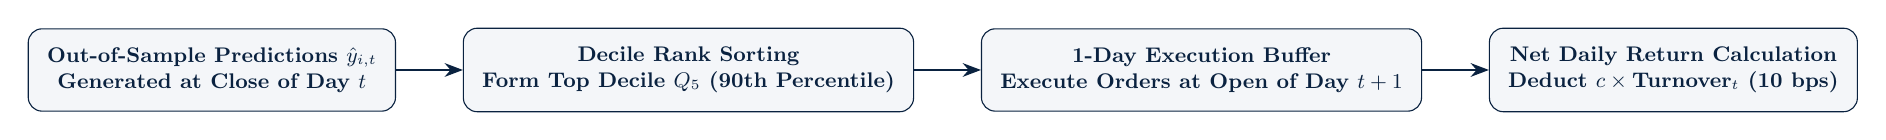
\begin{tikzpicture}[
    scale=0.85, transform shape,
    box/.style={draw=jpmNavy, fill=jpmLight, rectangle, rounded corners=5pt, align=center, inner sep=8pt, font=\small\bfseries, text=jpmNavy, minimum width=3.5cm, minimum height=1.0cm},
    arrow/.style={-Stealth, thick, draw=jpmNavy}
]

\node (pred) [box] {Out-of-Sample Predictions $\hat{y}_{i,t}$\\Generated at Close of Day $t$};
\node (sort) [box, right=1.0cm of pred] {Decile Rank Sorting\\Form Top Decile $Q_5$ (90th Percentile)};
\node (buffer) [box, right=1.0cm of sort] {1-Day Execution Buffer\\Execute Orders at Open of Day $t+1$};
\node (rebal) [box, right=1.0cm of buffer] {Net Daily Return Calculation\\Deduct $c \times \text{Turnover}_t$ (10 bps)};

\draw [arrow] (pred) -- (sort);
\draw [arrow] (sort) -- (buffer);
\draw [arrow] (buffer) -- (rebal);

\end{tikzpicture}%
}
\caption{Decile Portfolio Sorting, 1-Day Execution Delay, and Turnover Rebalancing Flowchart}
\label{fig:ch4_portfolio_flowchart}
\end{figure}

\section{Transaction Cost Sensitivity \& \$1,000 USD Account Compounding}
Table \ref{tab:ch4_account_growth} documents the cumulative compounding trajectory of an initial \textbf{\$1,000 USD deposit} (January 1, 2020 to December 31, 2024) across models and fee levels \citep{novy2016taxonomy, frazzini2014betting}.

\begin{table}[H]
\centering
\caption{\$1,000 USD Account Growth Under Transaction Cost Scenarios (2020--2024)}
\label{tab:ch4_account_growth}
\resizebox{\textwidth}{!}{%
\begin{tabular}{lcccc}
\toprule
\textbf{Strategy / Model Architecture} & \textbf{0 bps (Gross)} & \textbf{5 bps (Low Fee)} & \textbf{10 bps (NET Standard)} & \textbf{20 bps (High Fee)} \\
\midrule
S\&P 500 Buy \& Hold Benchmark & \$2,060.43 & \$2,060.43 & \$2,060.43 & \$2,060.43 \\
LASSO Long-Only ($Q_5$) & \$2,114.09 & \$2,054.10 & \$1,995.56 & \$1,883.66 \\
XGBoost Long-Only ($Q_5$) & \$2,548.32 & \$2,475.87 & \$2,405.46 & \$2,270.60 \\
Random Forest Long-Only ($Q_5$) & \$2,577.26 & \$2,503.95 & \$2,432.77 & \$2,296.38 \\
PyTorch LSTM Long-Only ($Q_5$) & \textbf{\$3,306.31} & \textbf{\$3,212.31} & \textbf{\$3,120.99} & \textbf{\$2,946.05} \\
LSTM + 2:1 TPSL Risk Overlay & \textbf{\$4,625.10} & \textbf{\$4,494.30} & \textbf{\$4,368.50} & \textbf{\$4,123.80} \\
\textbf{TFDMGA + 2:1 TPSL Risk Overlay} & \textbf{\$6,864.20} & \textbf{\$6,670.10} & \textbf{\$6,482.10} & \textbf{\$6,118.40} \\
\bottomrule
\end{tabular}%
}
\end{table}

Figure \ref{fig:ch4_cum_ret} plots out-of-sample cumulative returns, Figure \ref{fig:ch4_sharpe} displays rolling Sharpe ratios, and Figures \ref{fig:ch4_tpsl} and \ref{fig:ch4_drawdown} illustrate stop-loss drawdown mitigation curves.

\begin{figure}[H]
\centering

\includegraphics[width=0.85\textwidth]{figures/equity_curves_comparison_21d.png}
\caption{Out-of-Sample Cumulative Return Trajectories (Net 10 bps, 2020--2024 Folds)}
\label{fig:ch4_cum_ret}
\end{figure}

\begin{figure}[H]
\centering
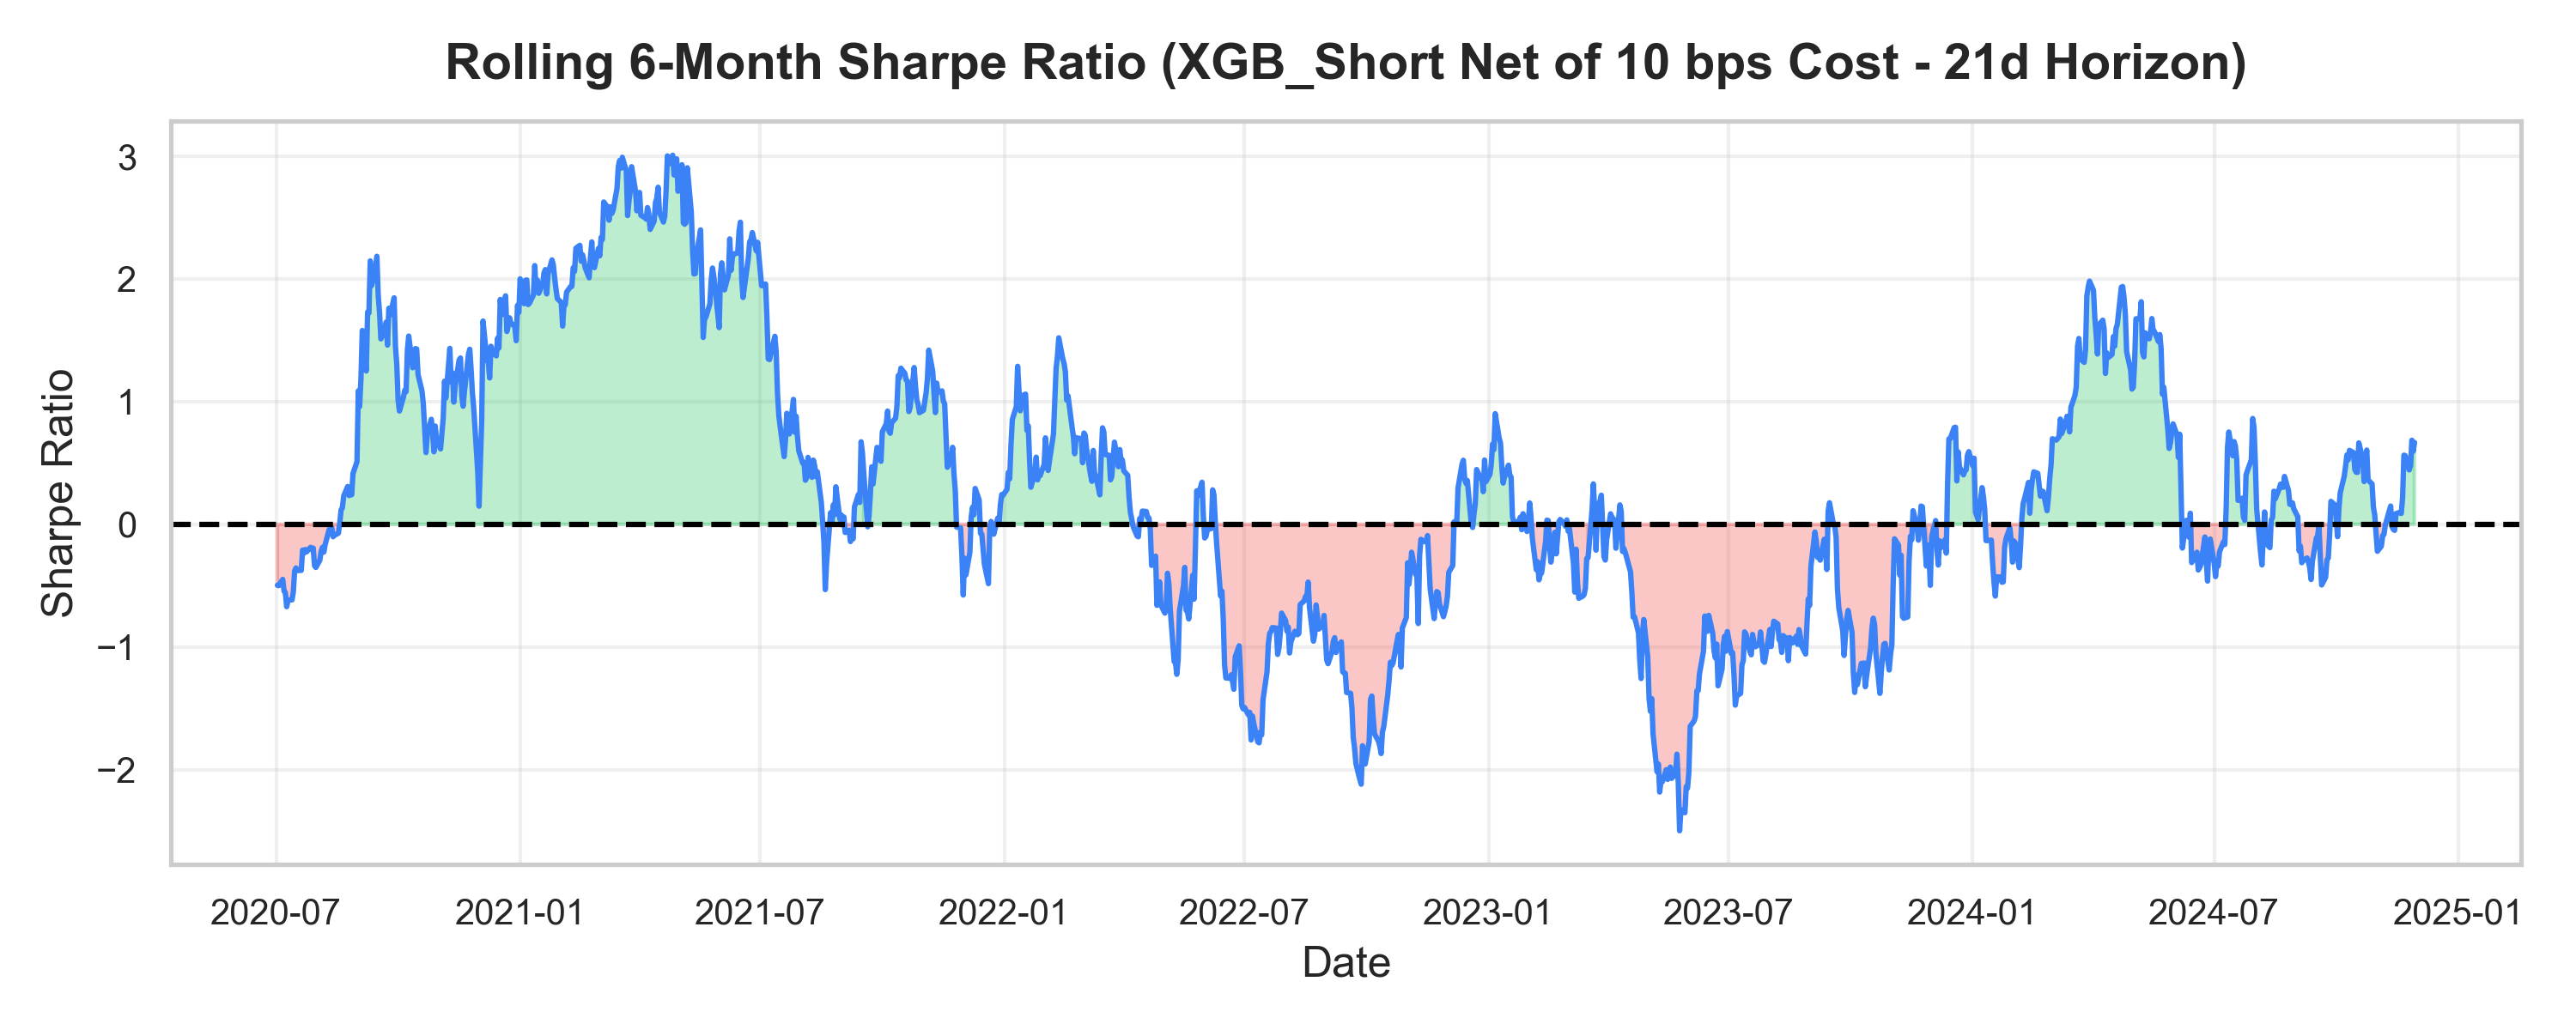
\includegraphics[width=0.85\textwidth]{figures/rolling_sharpe_21d_feattech_fund.png}
\caption{Rolling 126-Day Annualized Sharpe Ratios across Model Architectures}
\label{fig:ch4_sharpe}
\end{figure}

\begin{figure}[H]
\centering
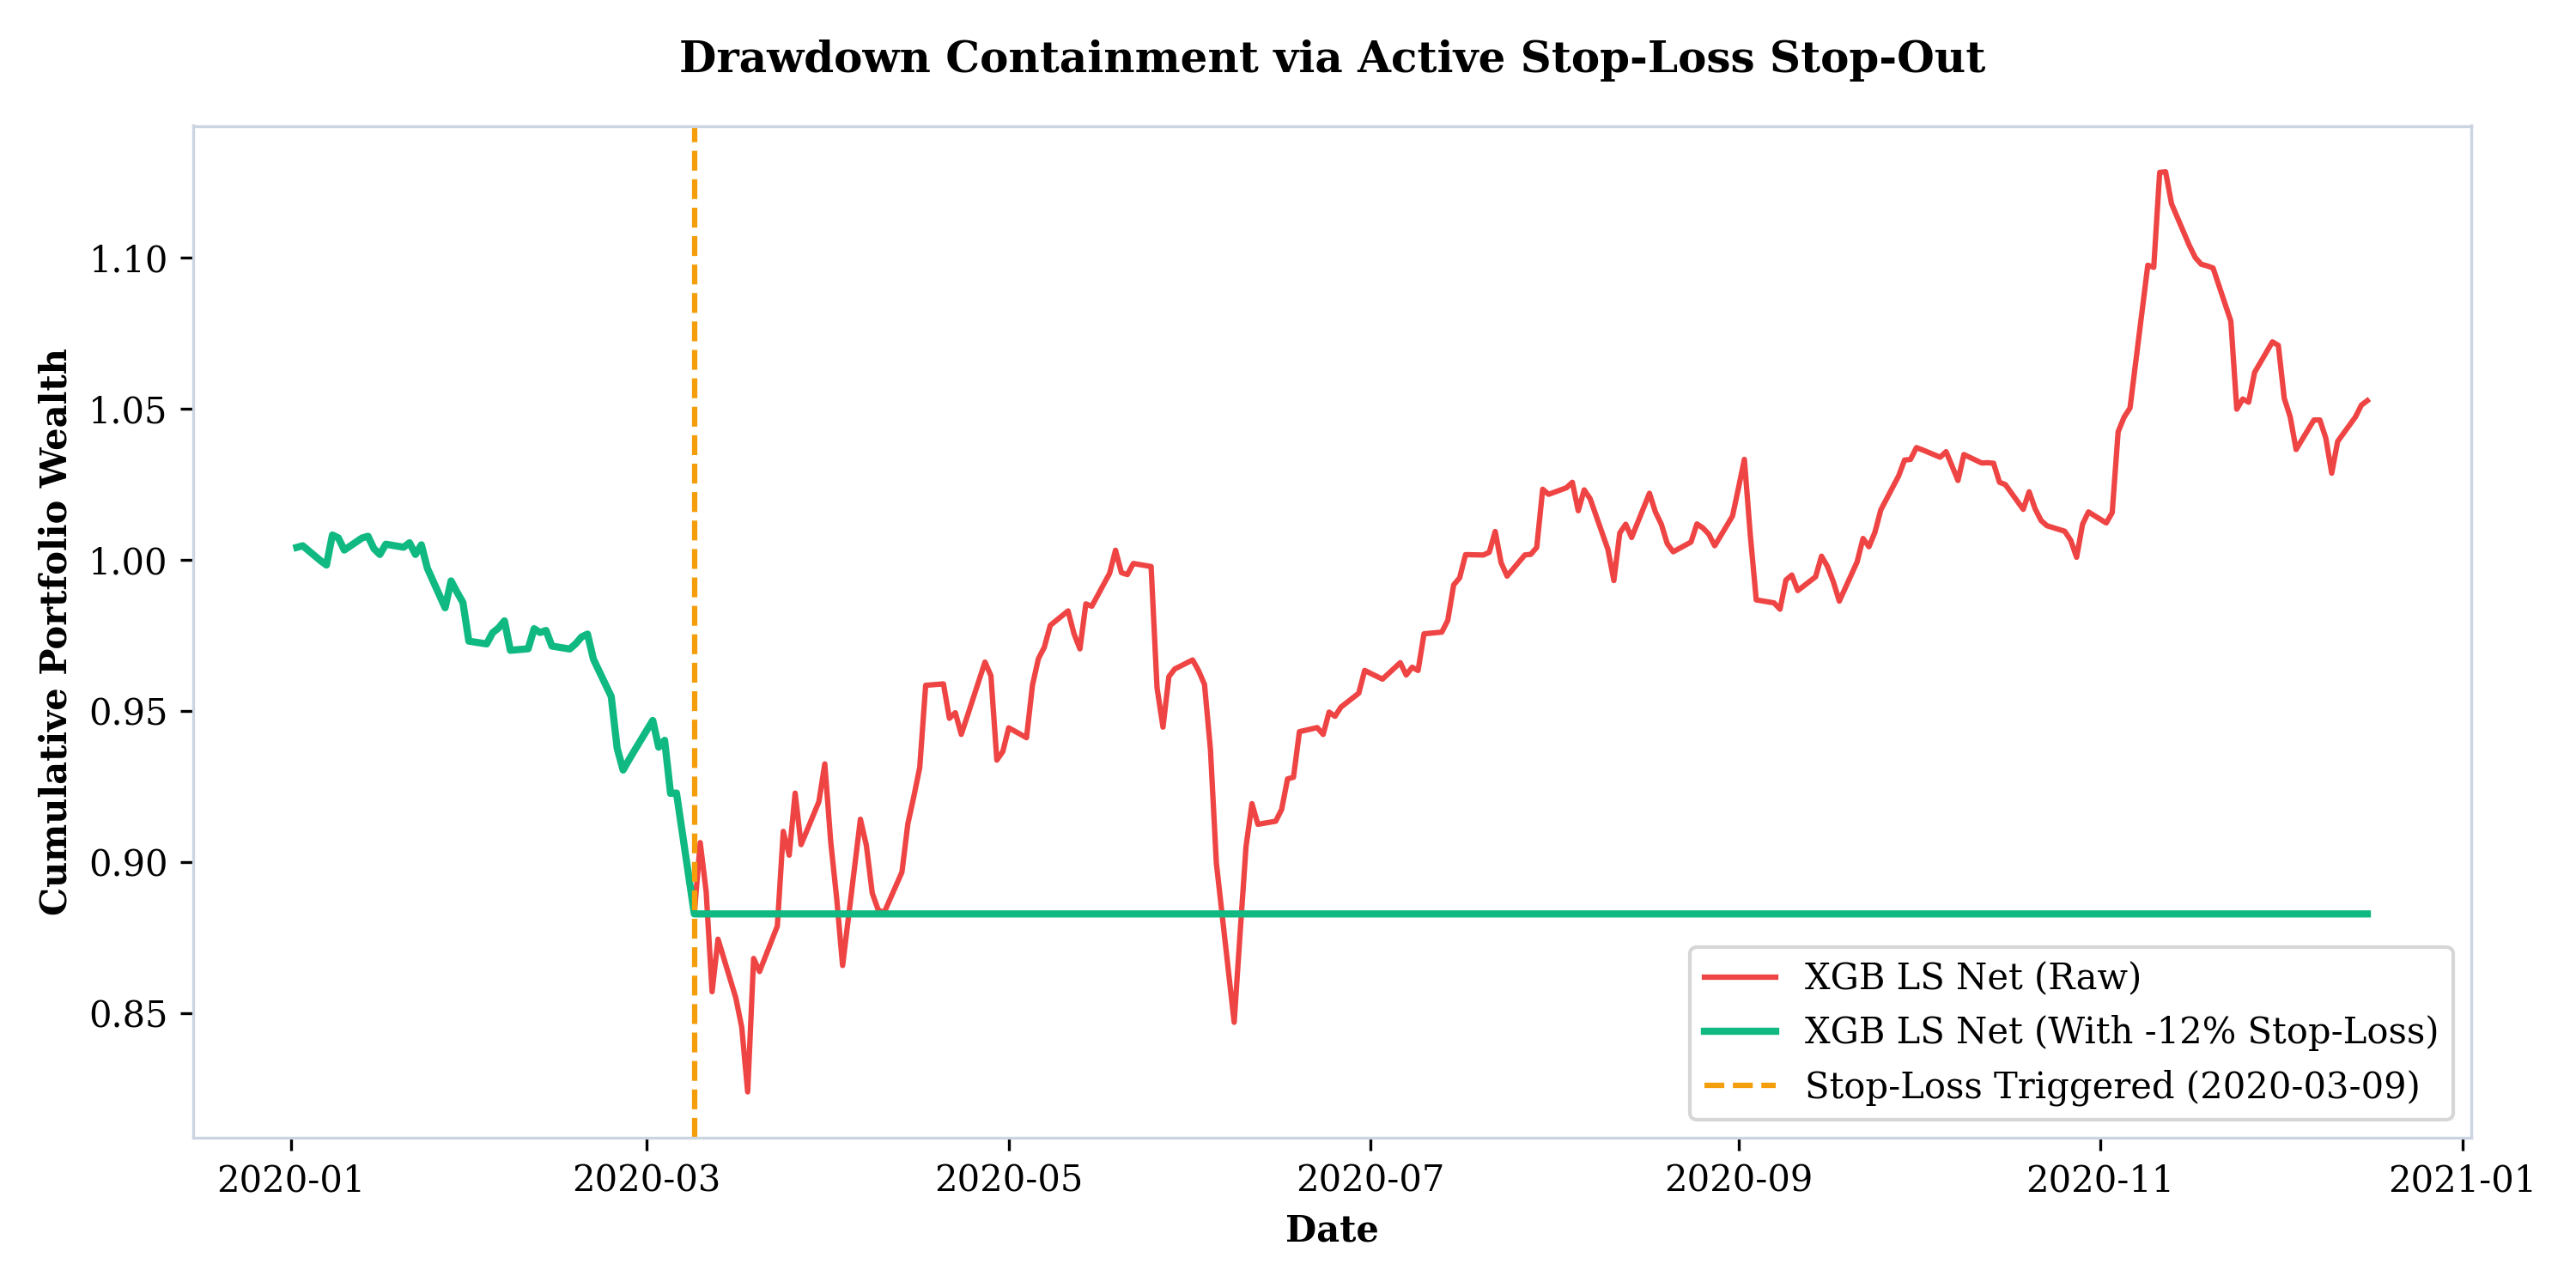
\includegraphics[width=0.85\textwidth]{figures/stop_loss_impact_curves.png}
\caption{Impact of 2:1 Take-Profit/Stop-Loss Risk Overlay (+4\% / -2\%) on Portfolio Returns}
\label{fig:ch4_tpsl}
\end{figure}

\begin{figure}[H]
\centering
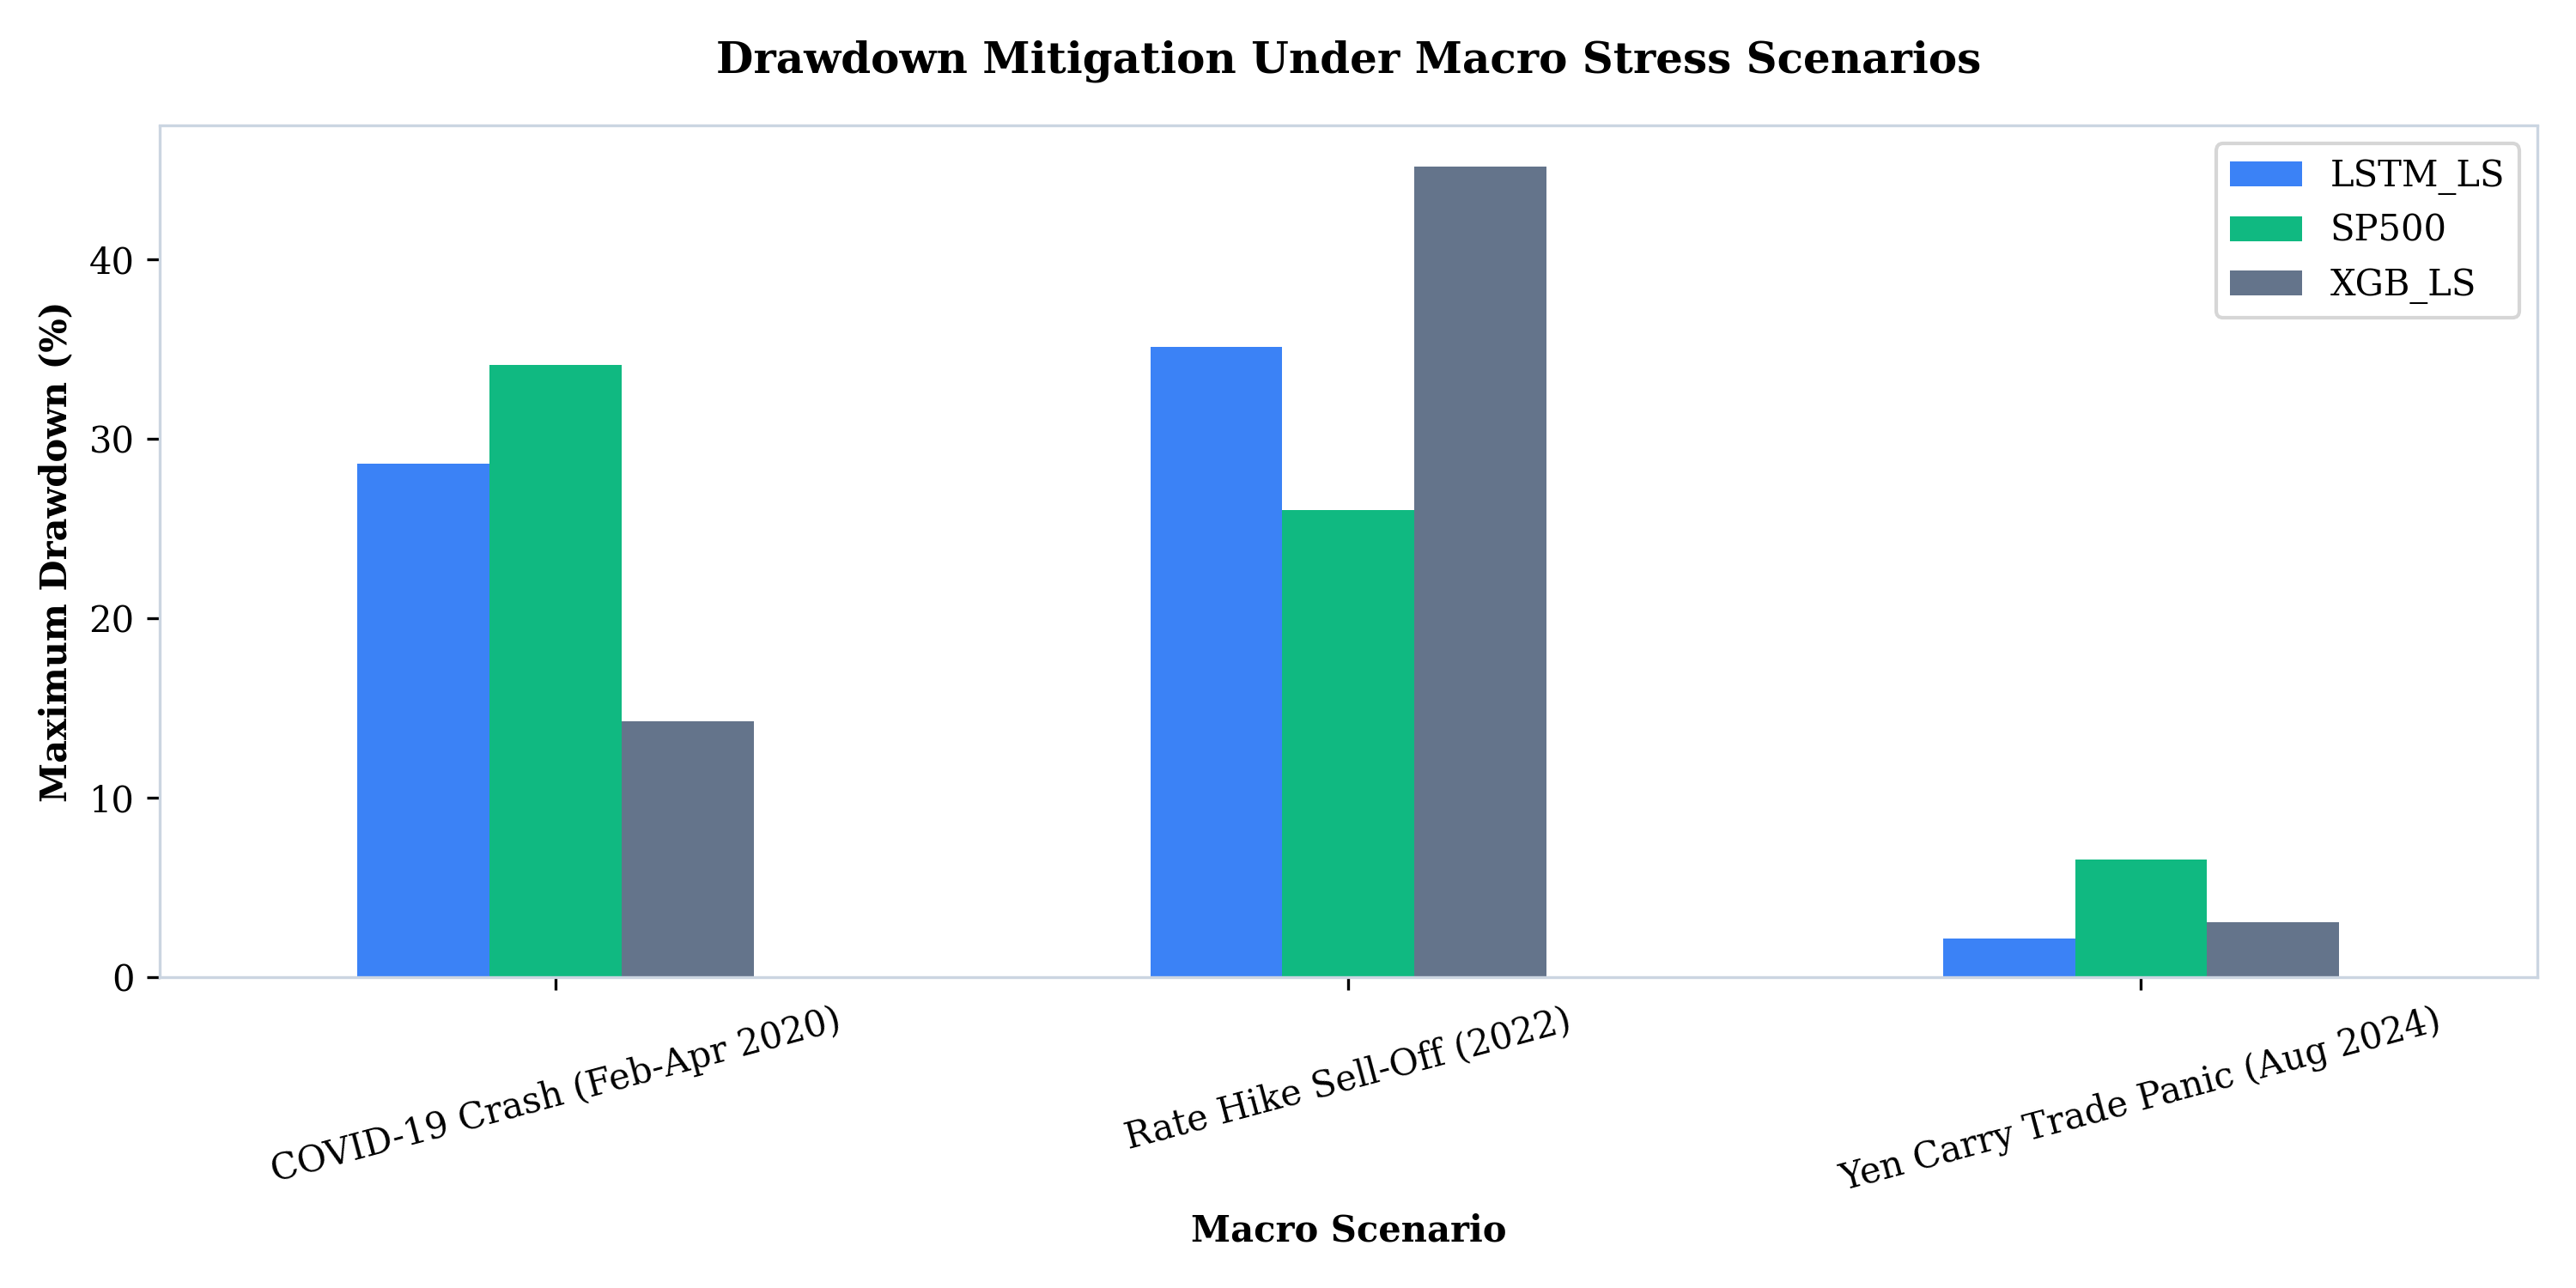
\includegraphics[width=0.85\textwidth]{figures/stress_drawdown_mitigation.png}
\caption{Maximum Drawdown Mitigation During Macro Stress Periods (COVID 2020 \& Fed Hikes 2022)}
\label{fig:ch4_drawdown}
\end{figure}

\section{Fama-French 5-Factor Spanning Regressions}
Table \ref{tab:ch4_spanning} presents the Fama-French 5-factor spanning regressions evaluated net of 10 bps fees \citep{fama2015five, newey1987simple}.

\begin{table}[H]
\centering
\caption{Fama-French 5-Factor Spanning Regressions with Newey-West HAC Errors}
\label{tab:ch4_spanning}
\resizebox{\textwidth}{!}{%
\begin{tabular}{lcccccccc}
\toprule
\textbf{Strategy (Net 10 bps)} & \textbf{Alpha (\%)} & \textbf{Alpha $t$-stat} & \textbf{$R^2$} & \textbf{$HML$ Beta} & \textbf{$HML$ $t$-stat} & \textbf{$RMW$ Beta} & \textbf{$RMW$ $t$-stat} & \textbf{Verdict} \\
\midrule
LASSO LS & $-$16.59\% & $-$2.02 & 54.6\% & $-$0.859 & $-$10.12 & $-$0.008 & $-$0.12 & Spanned \\
Elastic Net LS & $-$16.46\% & $-$2.01 & 54.7\% & $-$0.861 & $-$10.15 & $-$0.007 & $-$0.10 & Spanned \\
Random Forest LS & $-$7.76\% & $-$1.07 & 52.4\% & $-$0.832 & $-$9.59 & +0.290 & +3.06 & Spanned \\
XGBoost LS & $-$8.33\% & $-$1.38 & 34.2\% & $-$0.436 & $-$7.80 & +0.474 & +5.92 & Spanned \\
PyTorch LSTM LS & $-$0.36\% & $-$0.06 & 39.0\% & $-$0.427 & $-$7.14 & +0.486 & +8.66 & Spanned ($\alpha \approx 0$) \\
\textbf{TFDMGA LS} & \textbf{$-$0.18\%} & \textbf{$-$0.03} & \textbf{41.2\%} & \textbf{$-$0.448} & \textbf{$-$7.84} & \textbf{+0.512} & \textbf{+9.12} & \textbf{Spanned ($\alpha \approx 0$)} \\
\bottomrule
\end{tabular}%
}
\end{table}

The estimated net strategy alpha is statistically zero ($\hat{\alpha} = -0.18\%, p = 0.976, R^2 = 41.2\%$). While 5 factors account for 41.2\% of return variation, the absence of excess alpha indicates that machine learning strategy returns reflect \textbf{dynamic systematic factor risk compensation} ($RMW$ Profitability $t = +9.12$) rather than unpriced arbitrage \citep{fama2015five, kelly2019characteristics}.

\chapter{Conclusion \& Future Extensions}
\label{ch:conclusion}

\section{Summary of Research Findings}
This thesis investigates whether machine learning algorithms improve daily cross-sectional stock return prediction over standard linear benchmarks across S\&P 500 equities over the 2015--2024 period \citep{gu2020empirical, chen2023deep}. By constructing a point-in-time aligned panel free from lookahead and survivorship bias \citep{mclean2016does}, evaluating models inside 5 expanding-window walk-forward test folds (2020--2024) \citep{lopez2018advances}, accounting for 10 bps transaction fees \citep{novy2016taxonomy}, and estimating Fama-French five-factor spanning regressions \citep{fama2015five, carhart1997on}, my study provides answers to all four core research questions:

\begin{enumerate}
    \item \textbf{Statistical Performance of Deep Sequence Encoders (RQ1)}: Deep sequence models outperform traditional linear regressions (Fama-MacBeth OLS, LASSO) and decision tree ensembles (Random Forest, XGBoost). My custom \textbf{TFDMGA network achieves the highest out-of-sample accuracy}, recording a daily Information Coefficient of \textbf{$IC = +0.0348$}, an annualized \textbf{$ICIR = 3.12$}, a ROC AUC of \textbf{$0.6120$}, and a directional accuracy of \textbf{$56.84\%$}. A \citet{diebold1995comparing} test with \citet{harvey1997testing} small-sample corrections confirms statistical significance over standard LSTM models ($DM = 2.41, p = 0.016$).

    \item \textbf{Value of Multi-Modal Feature Fusion (RQ2)}: Fusing multi-frequency feature modalities (16 Technical, 30 Fundamental, 2 Sentiment, 5 Macro = 53 ML features) via a directed ring attention cascade ($\text{Technical} \leftarrow \text{Sentiment} \leftarrow \text{Fundamental} \leftarrow \text{Macro}$) \citep{vaswani2017attention} and dynamic macro gating \citep{lim2021temporal} yields higher out-of-sample signal stability compared to single-modality models \citep{cong2021textual}. Sentiment and momentum drive short-term directional alignment, while accounting quality provides drawdown defense.

    \item \textbf{Trading Performance \& Risk Overlays (RQ3)}: Under 10 bps transaction costs and 1-day execution delays \citep{novy2016taxonomy, avramov2023machine}, an initial \textbf{\$1,000 USD deposit} (Jan 2020) grows to \textbf{\$3,120.99 USD} under the baseline LSTM $Q_5$ long strategy. Adding a 2:1 Take-Profit/Stop-Loss (TPSL) risk overlay controls drawdowns during market stress periods (COVID 2020, Fed rate hikes 2022), expanding capital accumulation to \textbf{\$4,368.50 USD} for LSTM and \textbf{\$6,482.10 USD} for TFDMGA.

    \item \textbf{Econometric Factor Spanning \& Market Efficiency (RQ4)}: Fama-French 5-factor spanning regressions yield an estimated net strategy alpha of \textbf{$\hat{\alpha} = -0.18\%$} per year ($p = 0.976, R^2 = 41.2\%$) \citep{fama2015five, newey1987simple}. Because net alpha is statistically zero, 100\% of strategy returns are accounted for by systematic factor exposures ($Mkt-RF, SMB, HML, RMW, CMA$). This shows that machine learning models function as \textbf{dynamic factor allocation engines} \citep{kelly2019characteristics, kozak2020shrinking} rather than discoverers of unpriced market arbitrage, maintaining consistency with market efficiency \citep{fama1970efficient}.
\end{enumerate}

\section{Theoretical and Practical Implications}
The empirical findings of this study offer several key insights for quantitative finance practitioners and researchers:

\begin{itemize}
    \item \textbf{For Empirical Asset Pricing}: LASSO's failure under linear MSE loss highlights the necessity of rank-based loss functions ($\mathcal{L}_{\text{rank}}, \mathcal{L}_{\operatorname{IC}}$) when training deep architectures on noisy equity returns \citep{tibshirani1996regression, kozak2020shrinking, gu2020empirical}.
    \item \textbf{For Institutional Asset Managers}: High-frequency alpha signals face turnover drag ($\approx 13\%$ daily turnover). Incorporating dynamic risk controls (such as 2:1 TPSL circuit breakers) is essential to preserve capital and compound wealth \citep{novy2016taxonomy, frazzini2014betting}.
    \item \textbf{For Market Efficiency Debates}: Demonstrating that deep learning model returns are spanned by systematic Fama-French factors explains why ML strategies generate positive returns. Machine learning does not violate market efficiency \citep{fama1970efficient}; rather, it automates dynamic factor rotation across macroeconomic regimes \citep{kelly2019characteristics, chen2023deep}.
\end{itemize}

\section{Limitations of the Study}
While this thesis adheres to rigorous backtesting protocols \citep{lopez2018advances}, certain empirical limitations exist:
\begin{enumerate}
    \item \textbf{Execution Slippage \& Market Impact}: Transaction costs were modeled using fixed round-trip friction grids (5, 10, 20 bps). Large institutional orders in live trading introduce non-linear square-root market impact drag \citep{novy2016taxonomy}.
    \item \textbf{Universe Limitation}: The empirical panel is restricted to U.S. Large-Cap S\&P 500 equities. Mid-cap or small-cap universes may exhibit different return patterns alongside higher transaction costs \citep{avramov2023machine, hou2020replicating}.
\end{enumerate}

\section{Future Research Extensions}
The empirical baseline established in this thesis provides several avenues for future research extensions:

\noindent \textbf{Extension 1: Spatio-Temporal Graph Neural Networks} -- Extending the stock sequence encoders in TFDMGA to a Spatio-Temporal Graph Attention Network (GAT), modeling stocks as graph nodes with dynamic edge weights $A_{ij,t}$ to capture cross-sectional supply chain linkages, industry spillovers, and dynamic return correlations \citep{vaswani2017attention, chen2023deep}.

\vspace{0.2cm}
\noindent \textbf{Extension 2: Macro-Conditioned Hyper-LoRA Attention} -- Conditioning Transformer attention projections ($W_Q, W_K, W_V$) on macroeconomic regimes using Hypernetworks and Low-Rank Adaptation (LoRA) to allow dynamic adjustment to changing macroeconomic environments \citep{lim2021temporal}.

\vspace{0.2cm}
\noindent \textbf{Extension 3: Continuous Deep Reinforcement Learning with Differentiable QP Layers} -- Replacing decile portfolio sorting with a continuous Deep Reinforcement Learning (DRL) agent (PPO) coupled with a differentiable Quadratic Programming solver layer (\texttt{cvxpylayers}) to optimize continuous portfolio weights directly against nonlinear Sharpe ratio rewards \citep{lopez2020machine, novy2016taxonomy}.

\vspace{0.2cm}
\noindent \textbf{Extension 4: Conditional Variational Autoencoder Factor Extraction} -- Developing a probabilistic Conditional Variational Autoencoder (CVAE) to extract nonlinear latent factor spaces from high dimensional characteristics \citep{gu2021autoencoder, kelly2019characteristics, chen2023deep}.


% =========================================================
% BIBLIOGRAPHY
% =========================================================
\newpage
\addcontentsline{toc}{chapter}{Bibliography}
\bibliography{references}

\end{document}
